\chapter[Background Estimation][Background Estimation]{Background Estimation}
\label{chapter:background}

The \tth\ multi-lepton signal regions discussed in Chapter \ref{chapter:analysis} are contaminated by background contributions at a similar order of magnitude to the signal. The dominant background for each region is \ttV. Sub-dominant but important backgrounds include the production of vector boson pairs in associated with jets and b-quark jets ($VV$) and \ttbar\ production with a jet misidentified as a lepton (fakes). The 2$\ell$ SS regions possesses a unique background of charge misidentification from Z and top events. The methods for estimating these backgrounds are discussed in this chapter. Monte Carlo simulation is used for the prompt \ttV and $VV$ contributions. The non-prompt backgrounds from \ttbar\ jet-misidentification and charge-misidentification are estimated using data-driven methods. Table \ref{table:background_summary} provides a summary of the \tth\ signal and background expectation for each of the signal regions, including the data-driven estimates discussed in this section.


\begin{sidewaystable}[htbp]
\caption{Expected number of signal and background events in 2$\ell$ SS, 3$\ell$ and 4$\ell$ signal regions.}  
\resizebox{1.0\textwidth}{!}{%
\begin{tabular}{|c|c|c|c|c|c|c|c|c|c|}\hline 
                                       & \multicolumn{6}{c|}{Same-sign}                                         &  3 leptons    & \multicolumn{2}{c|}{4 leptons} \\
                                       &   \multicolumn{3}{c|}{$\geq 5$ jets}  &\multicolumn{3}{c|}{4 jets}     &                  & Z enriched & Z depleted \\ \hline
                                       &   \ee   &  \emu   & \mumu   &    \ee   &  \emu   & \mumu                &                       &  &           \\ \hline
\bf\tth                                & $0.73\pm0.03$  &  $2.13\pm0.05$ & $1.41\pm0.04$ & $0.44\pm0.02$ & $1.16\pm0.03$& $0.74\pm0.03$ & $2.34 \pm 0.04$   & $0.19 \pm 0.01$ & $0.03 \pm 0.00$     \\ \hline
\ttV                                   & $2.60\pm0.13$  & $7.42\pm0.17$  & $5.01\pm0.16$ & $3.05\pm0.13$ & $8.39\pm0.24$ & $5.79\pm0.20$ & $7.21 \pm 0.24$  & $0.74 \pm 0.05$ & $0.00 \pm 0.00$     \\ \hline
\tZ                                     & $$             & $$             & $$            &               &               &               & $0.71 \pm 0.03$ &   {\it incl. in \ttV}   & {\it incl. in \ttV} \\ \hline
$VV$                                     & $0.48\pm0.25$  & $0.37\pm0.23$  & $0.68\pm0.30$ & $0.77\pm0.27$ & $1.93\pm0.80$ & $0.54\pm0.30$ & $0.89 \pm 0.25$ &  $0.08 \pm 0.01$ & $0.00 \pm 0.00$     \\ \hline
fake leptons (DD)                      & $2.33\pm0.92$  & $6.66\pm1.06$  & $2.89\pm0.67$ & $3.45\pm1.36$ & $12.33\pm1.56$ & $6.32\pm1.26$ & $2.62 \pm 0.51$ &  $(1.1\pm0.6)\cdot10^{-3}$ & $(0.09\pm0.03)\cdot10^{-3}$ \\ \hline
Q misid (DD)                           & $1.10\pm0.09$  & $0.85\pm0.08$  & $-$  & $1.82\pm0.11$            & $1.39\pm0.08$ &  $-$  & $-$             &       $-$             & $-$                  \\ \hline \hline
Tot Background                         & $6.52\pm1.45$  & $15.30\pm1.64$ & $8.85\pm1.18$ & $9.07\pm1.42$ & $23.97\pm2.70$& $12.65\pm1.82$ & $11.43 \pm 0.62$&  $0.831\pm 0.075$& $0.0110\pm0.0003$  \\ \hline \hline
\end{tabular}
\label{table:background_summary}%
}
\end{sidewaystable} 


\section{Vector Boson ($W^{\pm}$, $Z$) production in association with top quarks: \ttV, \tZ}  
\label{section:ttV}
Production of top quarks plus vector boson is an important background in all multi-lepton channels.   A large part of the \ttV\ component, arising from on-shell $Z\to\ell\ell$, can be removed via a $Z$ mass veto on SFOS leptons.  However the $Z \to \tau\tau$ and $\gamma^*$ components remain. The \ttW\ and \tZ\ processes generally require extra jets to reach the multiplicity of our signal regions, as such it is important to ascertain uncertainties associated with QCD radation. We consider uncertainties on both the \ttW\ and \ttZ\ production cross-sections of these two processes and event selection efficiencies in the signal regions. The latter is sensitive to the NJet modelling in the MC. We assess the size of these uncertainties by investigating the effects of the choice of the factorization ($\mu_{\rm F}$) and renormalisation $\mu_{\rm R}$ scales and PDF sets. 

Monte Carlo events for these processes are generated with MadGraph 5 and showered with Pythia 6.  \ttW\ events are generated with up to two extra partons at matrix element level, while for \ttZ\ up to one extra parton at matrix-element level is produced.  The \tZ\ process is simulated without extra partons.  The next-to-leading-order (NLO) cross sections are implemented by applying a uniform $k$-factor to the leading-order (LO) events for each process.  For \ttZ, the $k$-factor is determined by comparing LO and NLO cross sections for on-shell $Z$ production only and then applied to the off-shell signal regions.  

The \ttV\ uncertainties are calculated
using the internal QCD scale and PDF re-weighting that is available with
 MadGraph5$+$aMC@NLO. The prescription for the scale envelope is taken from
\cite{Garzelli:2012bn}: the central value $\mu=\mu_{R}=\mu_{F}=m_t+m_V/2$
and the uncertainty envelope is $[\mu_{0}/2,2\mu_{0}]$. The PDF
uncertainty prescription used is the recipe from
\cite{Campbell:2012dh}: calculate the PDF uncertainty using the {\tt
MSTW2008nlo}~\cite{Martin:2009iq} PDF for the central value and then the final PDF
uncertainty envelope is derived from three PDF error sets each with
different $\alpha_S$ values (the central value and the upper and lower
90\% CL values). The final NLO cross section central values and
uncertainties are given in Table~\ref{tab:ttVXSunc}.

\begin{table}%[ht!!!]
\begin{center}
\caption{NLO cross section and theoretical uncertainty
  calculations derived from MadGraph5$+$aMC@NLO.}
\label{tab:ttVXSunc}
\begin{tabular}{l|p{0.15\textwidth}|p{0.1\textwidth}|p{0.1\textwidth}|p{0.1\textwidth}|p{0.1\textwidth}|p{0.2\textwidth}}
\hline
Process & $\sigma_{NLO}$ [$fb$] & \multicolumn{2}{c|}{Scale
Uncertainty [\%]} & \multicolumn{2}{c|}{PDF Uncertainty [\%]} & Total
symmetrized uncertainty [\%] \\
\hline
\hline
$t\bar{t}W^{+}$ & 144.9 & +10 & -11 & +7.7 & -8.7 & 13.3 \\
$t\bar{t}W^{-}$ & 61.4  & +11 & -12 & +6.3 & -8.4 & 13.6 \\
$t\bar{t}Z$     & 206.7 & +9  & -13 & +8.0 & -9.2 & 14.0 \\
$tZ$            & 160.0 & +4  & -4  & +7   & -7   & 8.0 \\
$\bar{t}Z$      & 76.0  & +5  & -4  & +7   & -7   & 8.6 \\
\hline
\end{tabular}
\end{center}
\end{table}

The \tZ\ process is normalized to NLO based on the calculation in Ref.~\cite{Campbell:2013yla}.  Here the scales are set to $\mu_0 = m_t$ and the scale variations are by a factor of four; the scale dependence is found to be quite small.


\subsection{\ttZ\ Validation Region}

Unlike \ttW\, a \ttZ\ validation region can be obtained by simply inverting the veto on SFOS lepton pairs near the Z pole in the 3 lepton signal region. This region thus requires 3 leptons (with momentum and identification cuts discussed in Chapter \ref{chapter:selection}, at least one SFOS pair of leptons within 10 GeV of the Z mass, and either 4 jets and at least 1 b-tagged jet or exactly 3 jet and 2 or more b-tagged jets. The resulting region has low statistics and is not used as a control region but is instead used as a validation to demonstrate that the normalization uncertainty, discussed above, is properly evaluated. 

The region defined by this is predicted to be 67\% \ttZ, 17\% \WZ, and 13\% \tZ.  We predict $19.3 \pm 0.5$ events and observe 28, giving a observed-to-predicted ratio of $1.45 \pm 0.27 \pm 0.03$, where the errors are from data and simulation statistics, respectively. Given the large errors, the region is still in agreement with the predictions to within 1-1.5 $\sigma$.  Distributions of various variables are shown in Fig.~\ref{figure:background_ttZCRA}.  

\begin{figure}
 \begin{center}
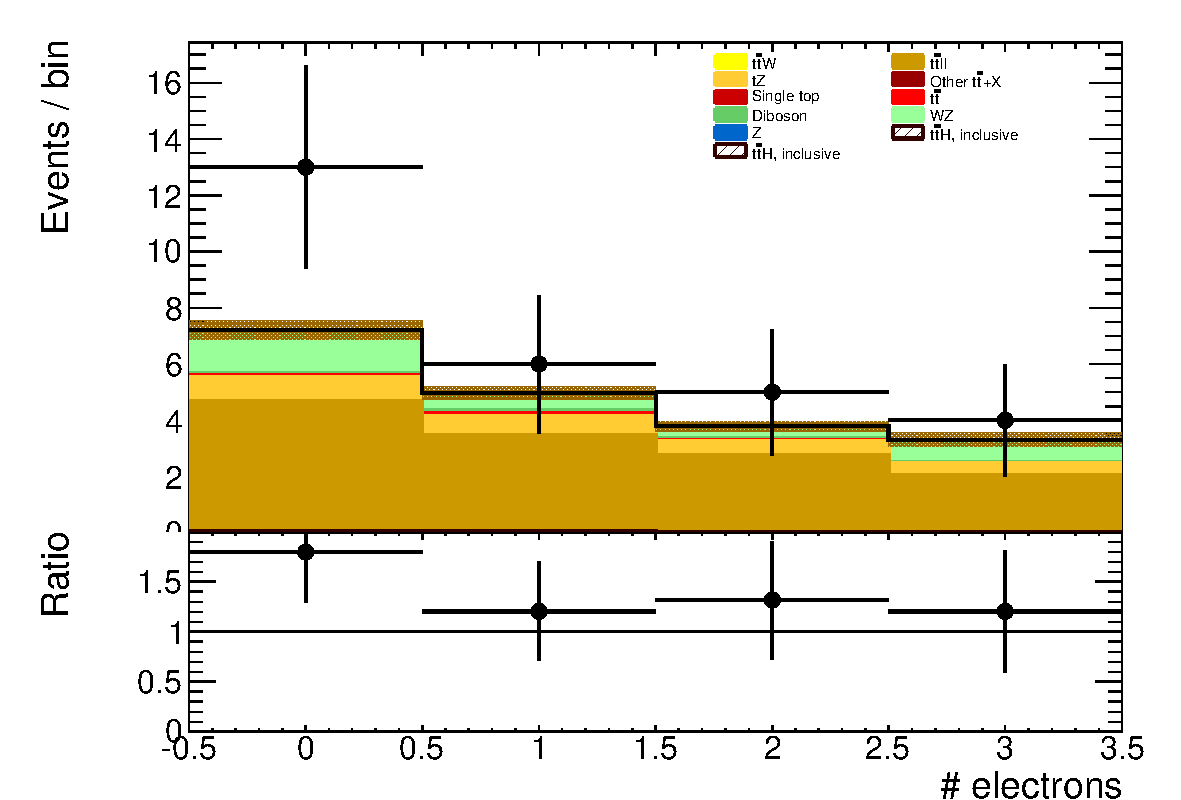
\includegraphics[width=.5\linewidth]{figs/ttZ/ttz_3l_CR_nelec}%
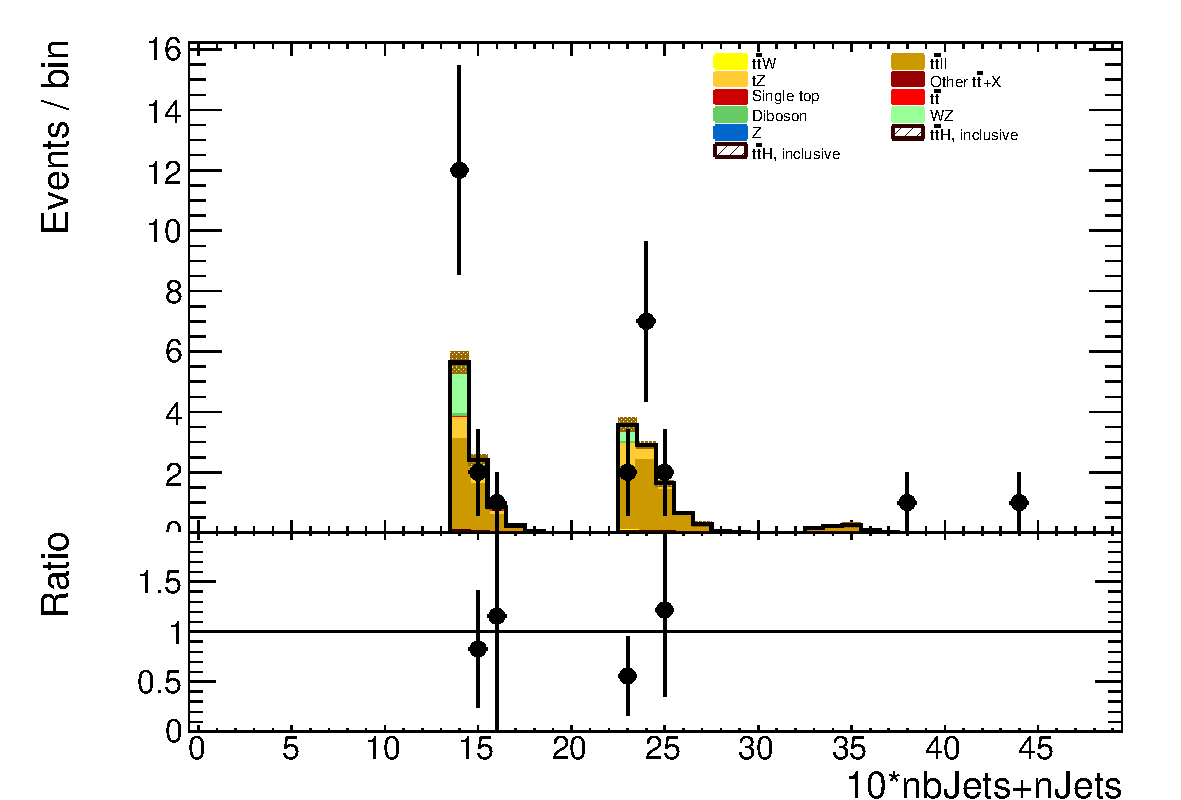
\includegraphics[width=.5\linewidth]{figs/ttZ/ttz_3l_CR_nJets_and_nbJets_lin}\\
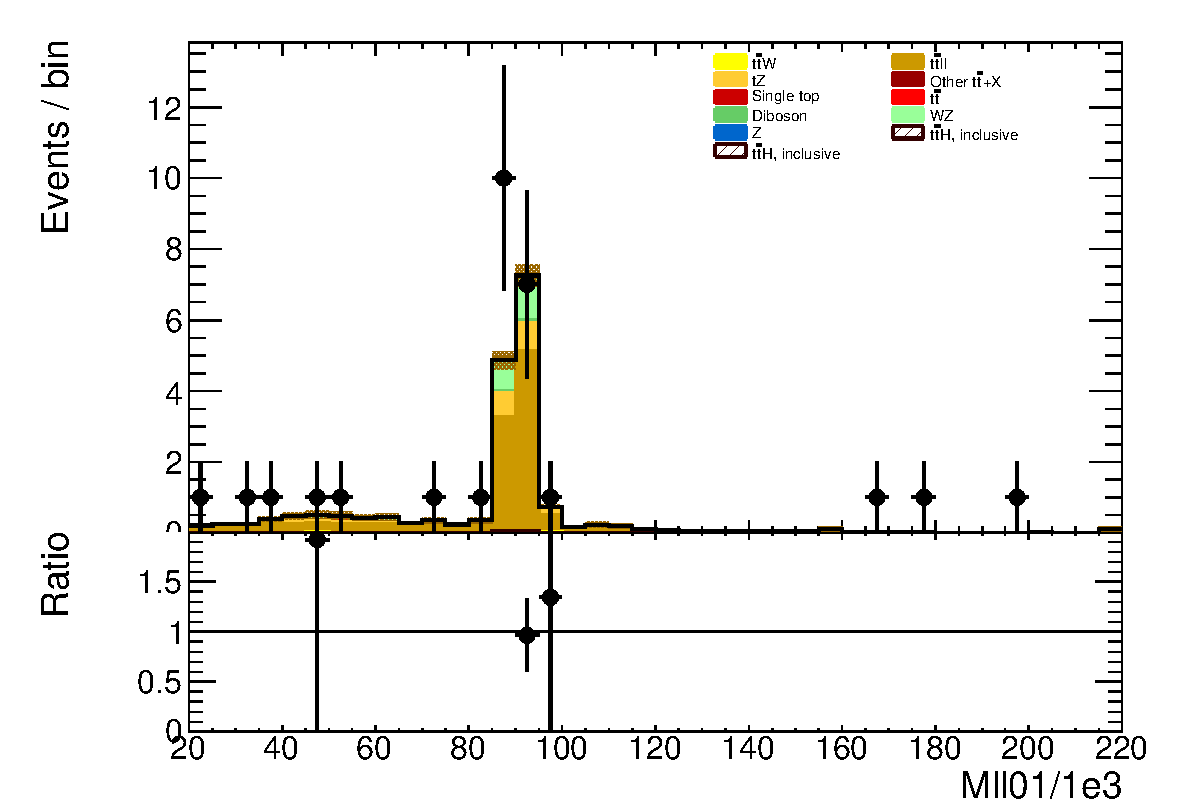
\includegraphics[width=.5\linewidth]{figs/ttZ/ttz_3l_CR_Mll01}%
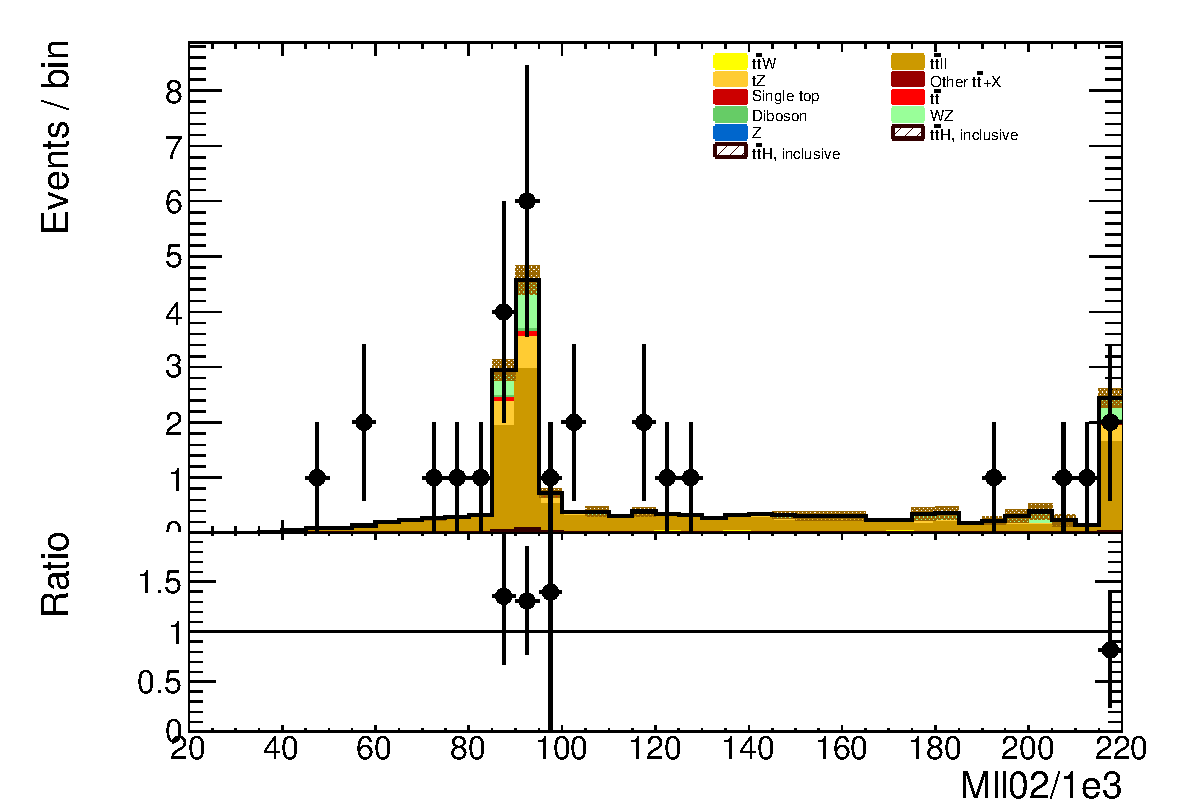
\includegraphics[width=.5\linewidth]{figs/ttZ/ttz_3l_CR_Mll02}\\
  \caption{\label{figure:background_ttZCRA}Data/MC comparison plots for \ttZ\ control region A ($\ge4$ jets, $\ge1$ $b$-tag and 3 jets, $\ge 2$ $b$-tag). In all plots, the rightmost bin contains any overflows.  Top left: number of electrons.  Top right: 10*the number of $b$-tags + the total number of jets. Middle left: the invariant mass of the (0,1) lepton pair (see the text for the definition of the lepton ordering).  Middle right: the invariant mass of the (0,2) lepton pair.}
 \end{center}
\end{figure}



\section{Di-boson Background Estimation: \WZ, \ZZ }

\label{section:wz}
$W^{\pm}Z$ and $ZZ$ di-boson production with additional and b-tagged jets constitute small contributions to 
the 3$\ell$ and 4$\ell$ channels. For the 3$\ell$ case $W^{\pm}Z$ comprises $\sim$ 10\% of the total background, while for
the 4$\ell$ case $ZZ$ contribution accounts comprises $\sim$ 10\% of the total background. 
Because of the small size of these contributions, each of the above processes can be assigned a 
non-aggressive uncertainty based on similar previous analyses with ATLAS and cross-checked with data validation 
regions and MC truth studies. 

Both $W^{\pm}Z$ and $ZZ$ production have been studied by ATLAS \cite{WZAtlas}\cite{ZZAtlas}, but neither process
has been investigated thoroughly in association with multiple jets and b-quark jets. However, single boson production with
b-quark jets has been investiaged. Both $W+b$ \cite{WbAtlas} 
and $Z+b$ \cite{ZbAtlas} production in 7 TeV data have been shown to agree with MC models to within 20-30\%. 

A single $W$ produced in association with b-tagged jets possesses a similar topology to the $W^{\pm}Z+b$ 
process at a different energy scale and has been shown to be dominated by c mis-tags and b-jets from gluon splitting 
and multiple parton interaction. The $W+b$ analysis, referenced above, uses Alpgen MC with Herwig PS modeling, only provides
results to 1 additional jet, and uses the CombNN tagger (we use MV1). Its results are therefore not directly comparable to this \tth\ analysis (where $W^{\pm}Z$ is modeled using Sherpa with massive c and b quarks). $Z+b$ production originates from slightly different diagrams than $ZZ+b$, but the sources of the b-tags are similar. The 7 TeV analysis, referenced above, provides results with Sherpa MC with an agreement of $\sim$ 30\%. However, it also used the CombNN tagger instead of MV1. Beause of the differences of the 2011 single boson analyses (type of tagger used, type of MC and tunes used), we would like to verify the general 20-30\% level of agreement in 2012 data with the simulation and tagger used in the \tth\ analysis: Sherpa MC, 2012 tunes, MV1. With the data skims available to use we are able to do this in the $Z+b$ region but not the $W+b$.  


Figure \ref{figure:background_wz_zb} shows the spectrum of the number of reconstructed and selected jets (NJet) in a 
$Z+b$ validation region, defined by 2 tight-isolated leptons within 10 \gev of the Z mass and with at 
least one b-tagged jet, using the \tth\ analysis definitions. The level of agreement in this region confirms 
at the  30\% level seen in the 7 TeV analysis, discussed above. 

\begin{figure}[!htbp]
\centering 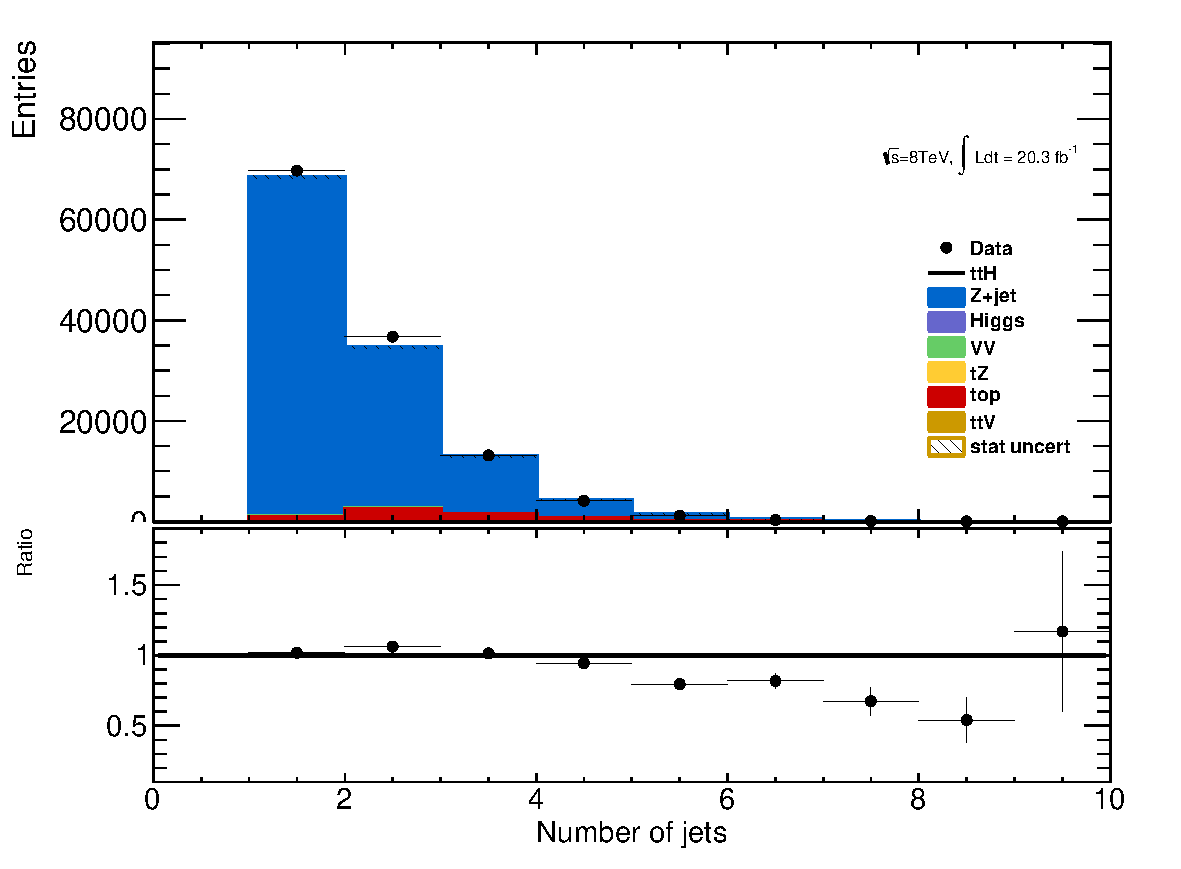
\includegraphics[width=0.5\textwidth]{figs/wz/ZbVR}
\caption{NJet spectrum for 2 tight-isolation leptons with 1 b-tagged jet (MV1\_70)} 
\label{figure:background_wz_zb}
\end{figure} 

In the following two sections, we assess the truth origin of jets in the $W^{\pm}Z+b$ and $ZZ+b$ regions and leverage data/MC agreement where we can. We see that the data allows us to constrain the \WZ\ to 50\%. We claim this 50\% as a systematic. The 20-30\% agreement in the single boson regions above bolsters our confidence in this number. 

\subsection{$W^{\pm}Z$ Normalization Uncertainty} 
The \tth\ analyses has two validation regions to test the Sherpa agreement with data for $W^{\pm}Z$: one inclusive 3 lepton region, using the three-lepton channel object and \pt\ cuts and a $W^{\pm}Z+b$ region with 1 b-tagged jet and a requirement that at least one SFOS pair have an invariant mass within 10 GeV of the Z mass. The region with fewer than 4 jets is \WZ\ dominated. Figure \ref{figure:background_wz_incl} shows kinematic variables for the inclusive region. The overall data normalization is $\sim$10\% higher than MC, but this will be well within our systematic uncertainty. The NJet shape shows good agreement across the full spectrum, giving confidence about the Sherpa high NJet SR extrapolation. Figure \ref{figure:background_wz_z_b} shows NJet spectrum for the $W^{\pm}Z+b$ validation region with agreement with in statistical uncertainties. The region has low statistics and around $\sim$ 60\% purity and statistical analysis of the region suggests that a 50\% normalization error on the \WZ\ component is enough to cover any possible mismodelings, especially in higher NJet bins, which are closer to the signal regions.  

\begin{figure}[!htbp]
  \begin{minipage}[h]{0.5\textwidth}
    \centering 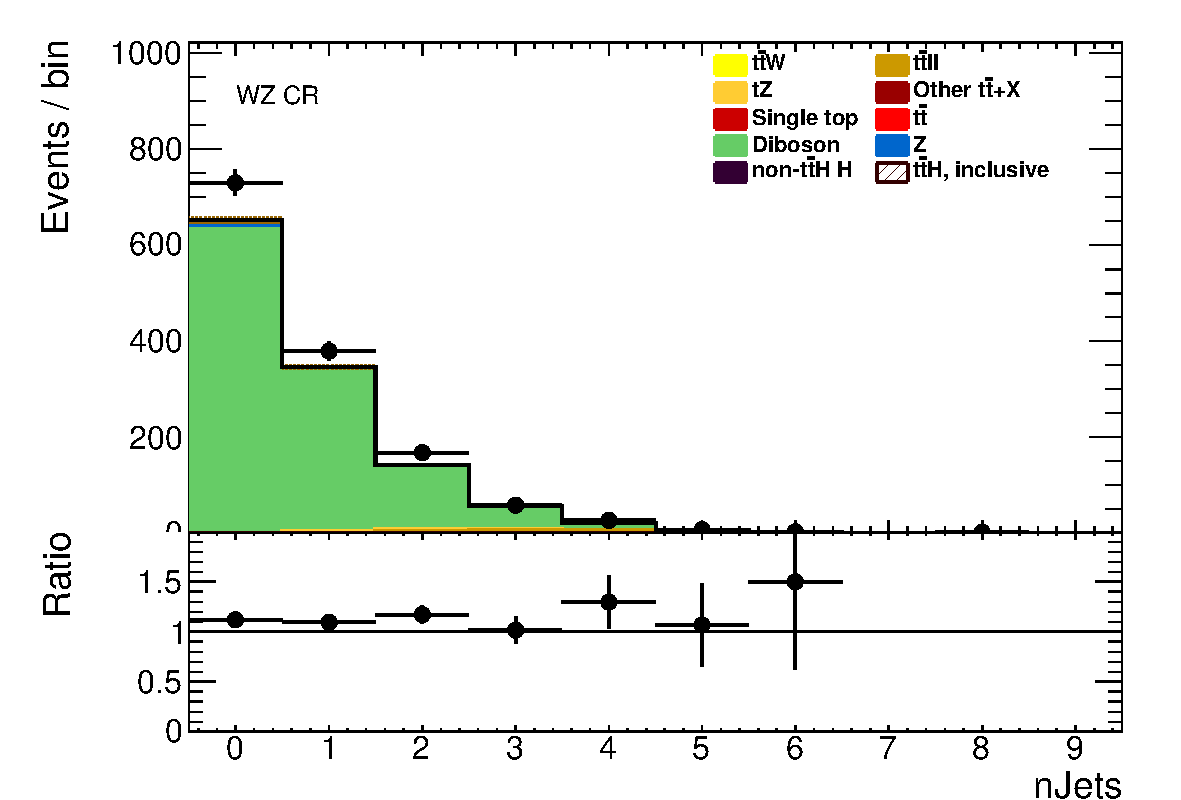
\includegraphics[width=\textwidth]{figs/WZ/standardCR_3l_WZ_MT_nJets_OR_thesis}
  \end{minipage}\hfill
  \begin{minipage}[h]{0.5\textwidth}
    \centering 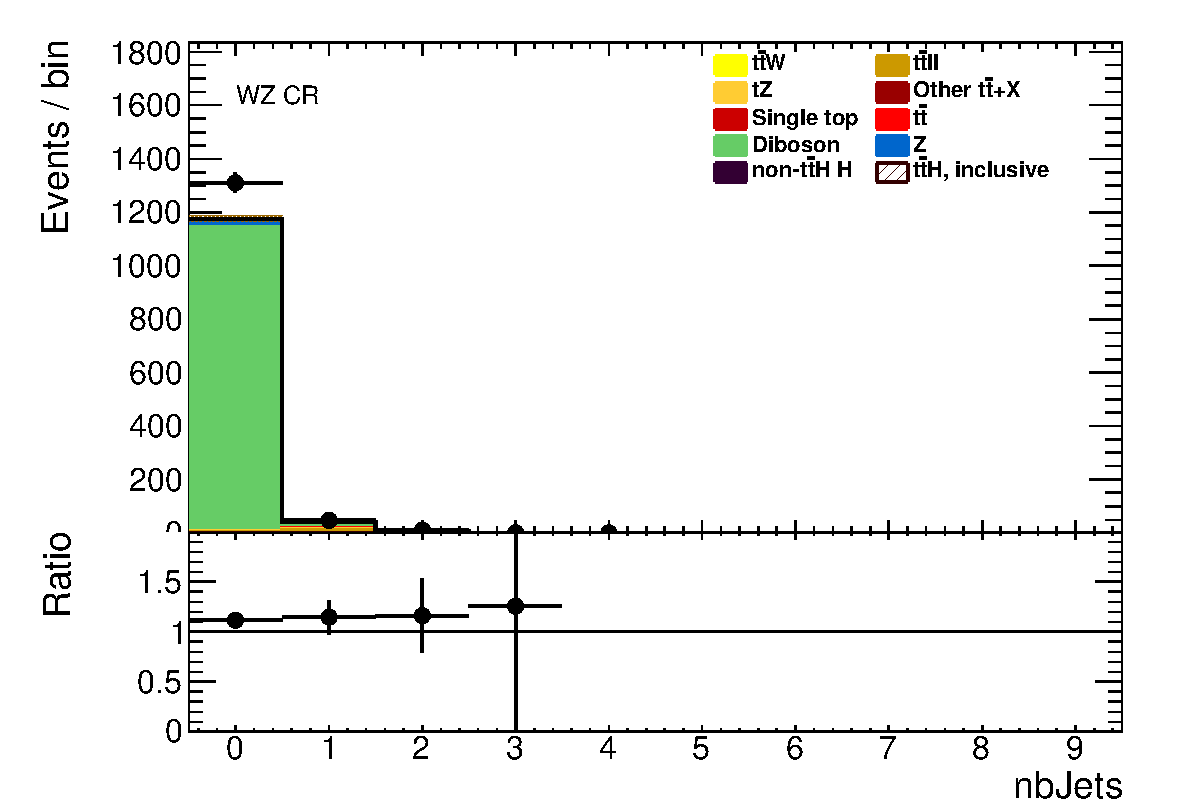
\includegraphics[width=\textwidth]{figs/WZ/standardCR_3l_WZ_MT_nJets_OR_MV1_70_thesis}
  \end{minipage}\hfill
  \begin{minipage}[h]{0.5\textwidth}
    \centering 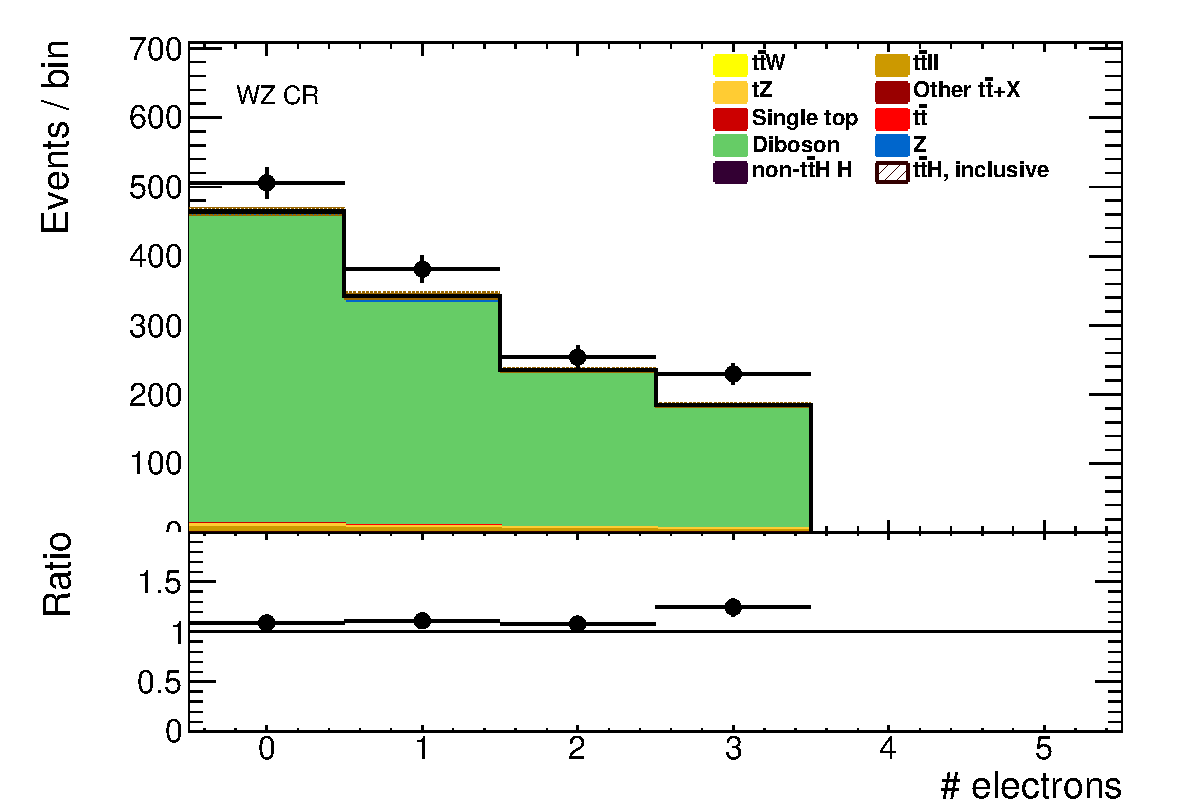
\includegraphics[width=\textwidth]{figs/WZ/standardCR_3l_WZ_MT_nelec_thesis}
  \end{minipage}\hfill
  \begin{minipage}[h]{0.5\textwidth}
    \centering 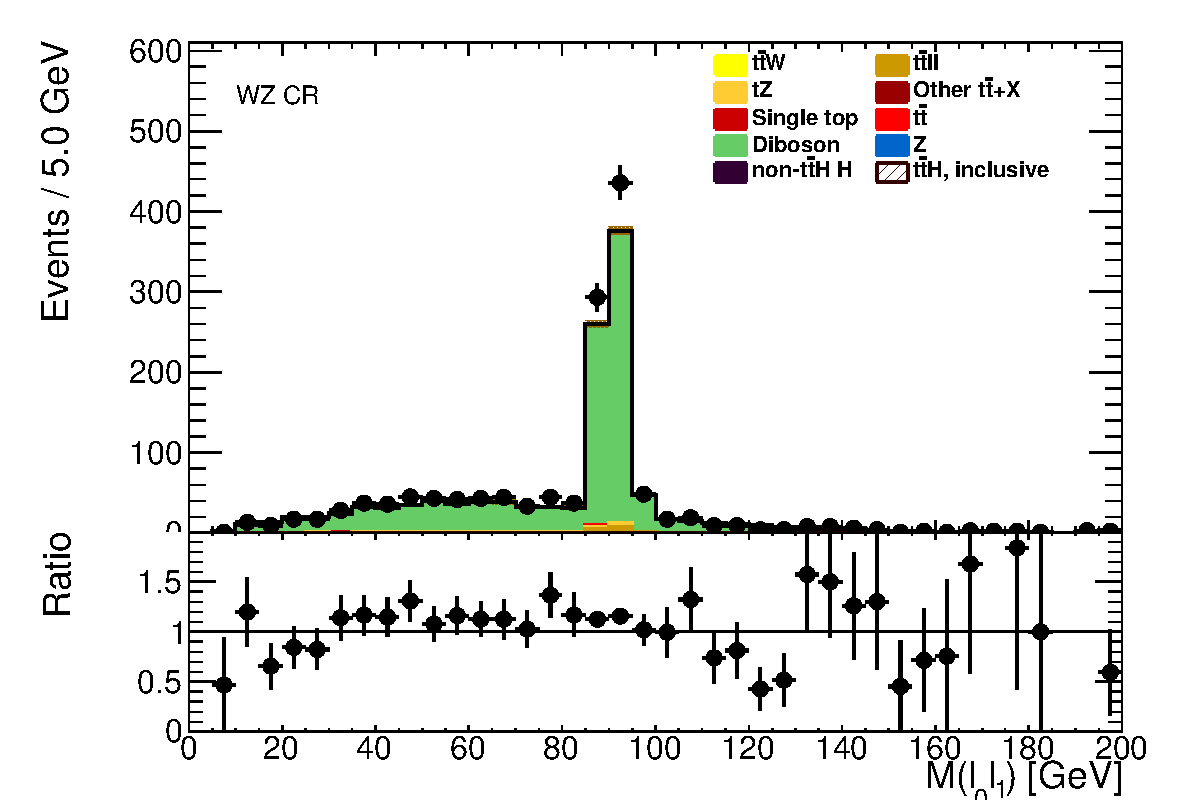
\includegraphics[width=\textwidth]{figs/WZ/standardCR_3l_WZ_MT_Mll01_thesis}
  \end{minipage}\hfill

\caption{3 lepton $W^{\pm}Z$ validation using the \tth\ lepton identification and momentum cuts: mass, number of jet and flavor variables} 
\label{figure:background_wz_incl}
\end{figure} 



\begin{figure}[!htbp]

  \begin{minipage}[h]{0.5\textwidth}
    \centering 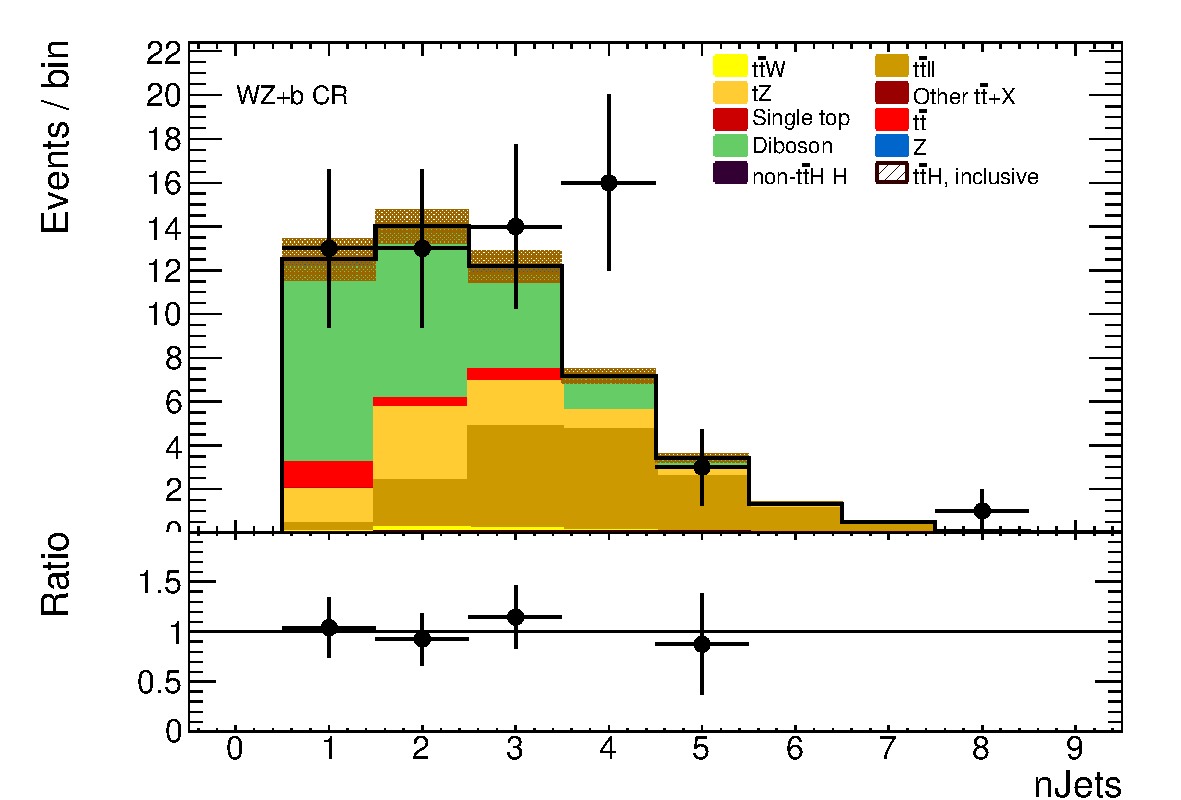
\includegraphics[width=\textwidth]{figs/WZ/standardCR_3l_WZ_MT_1b_nJets_OR_thesis}
  \end{minipage}\hfill
  \begin{minipage}[h]{0.5\textwidth}
    \centering 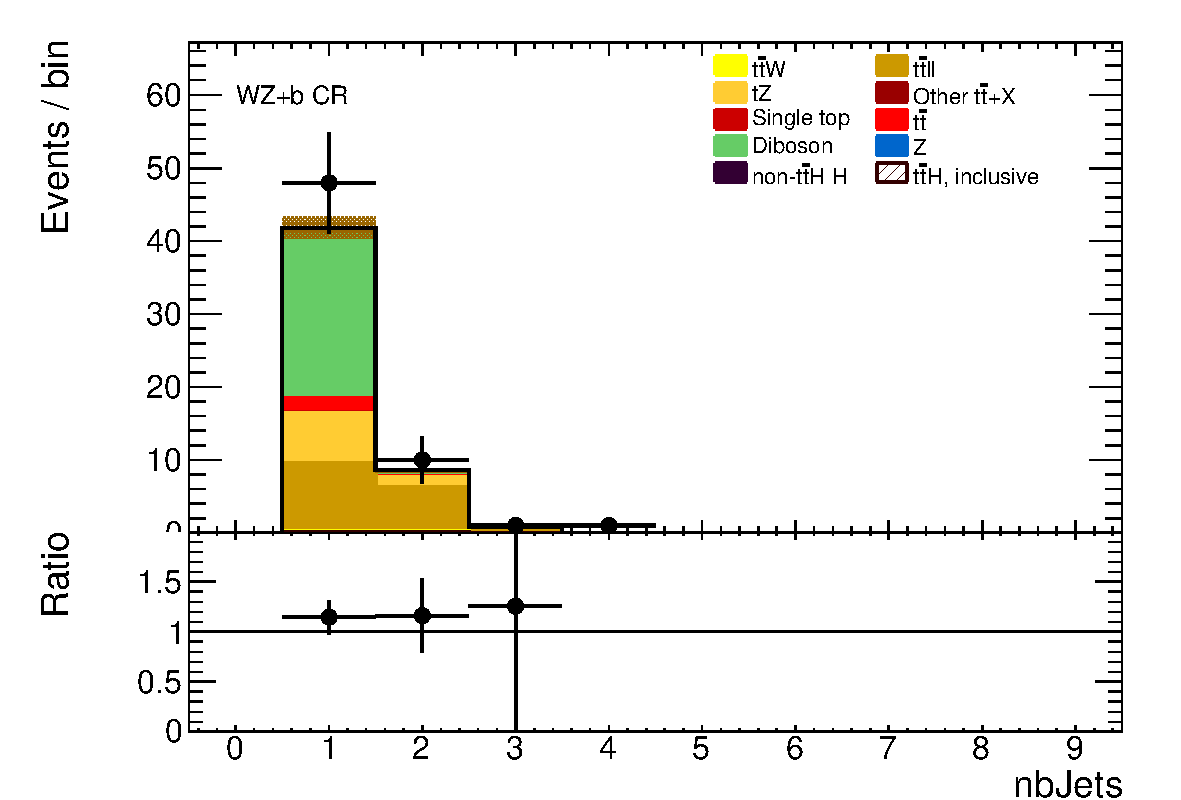
\includegraphics[width=\textwidth]{figs/WZ/standardCR_3l_WZ_MT_1b_nJets_OR_MV1_70_thesis}
  \end{minipage}\hfill
  \begin{minipage}[h]{0.5\textwidth}
    \centering 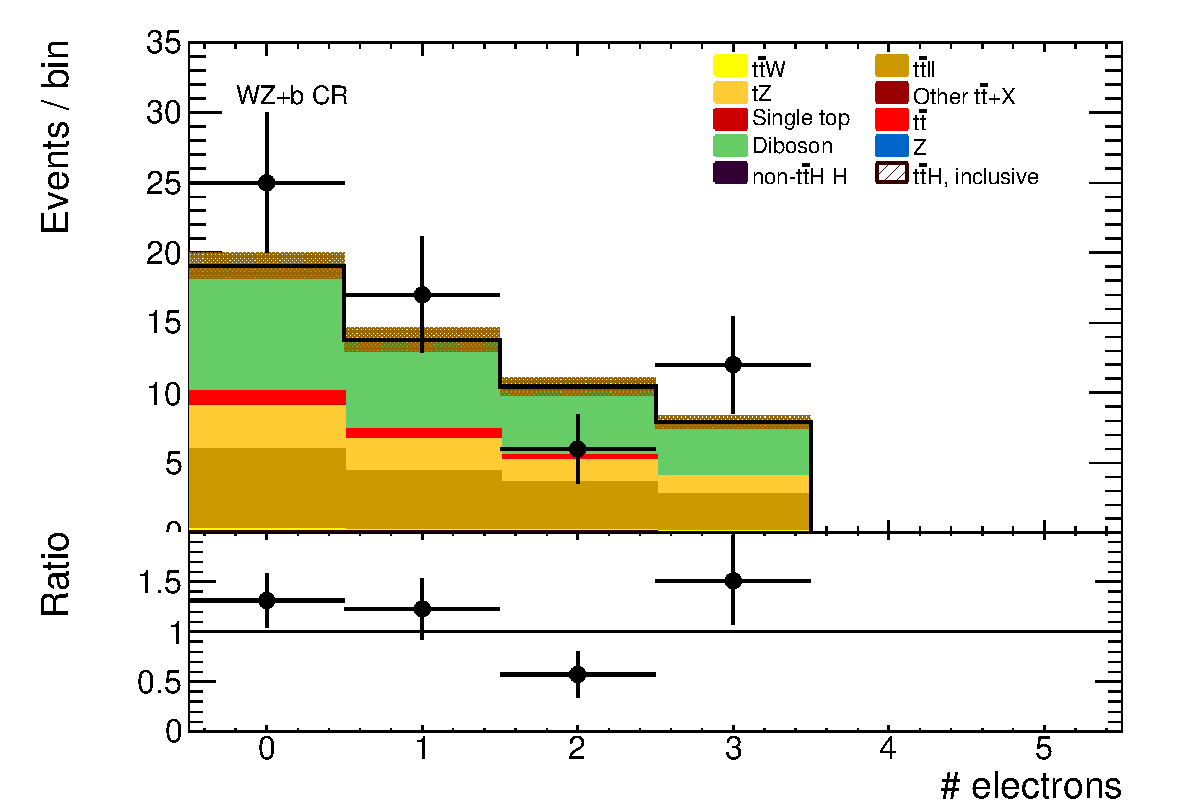
\includegraphics[width=\textwidth]{figs/WZ/standardCR_3l_WZ_MT_1b_nelec_thesis}
  \end{minipage}\hfill
  \begin{minipage}[h]{0.5\textwidth}
    \centering 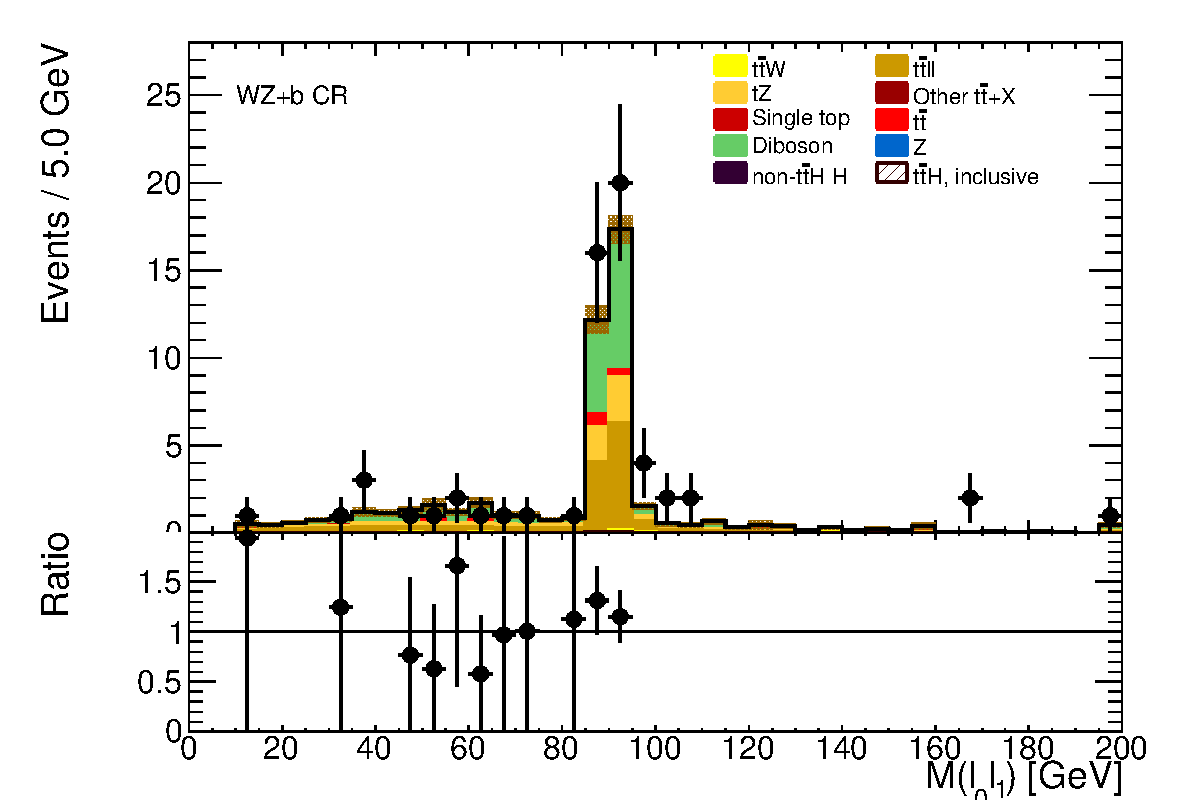
\includegraphics[width=\textwidth]{figs/WZ/standardCR_3l_WZ_MT_1b_Mll01_thesis}
  \end{minipage}\hfill
\caption{$W^{\pm}Z+b$ validation region: NJet, NElec, and Mass Variables} 
\label{figure:background_wz_z_b}
\end{figure} 

We also examine the $W^{\pm}Z$ truth origins of the b-jet in the $W^{\pm}Z+b$ validation region (VR) and the signal region using MC to assess the validity of the extrapolation from the VR to the SR and to confirm the similarity in jet origin to the single boson analyses, references above. The flavour of the closest matching truth particle ($p_T > 5$ GeV, after FSR) in $\Delta R$ determines the true-jet flavor. If there are no quarks, taus or gluons within $\Delta R$ of 0.3, the label defaults to light.  Table \ref{table:wz_truth} shows the origin fraction of b-tagged jets in the various $W^{\pm}Z+b$ VRs and the SR. If there are two b-tagged jets, the highest \pt\ is used, but this is a small fraction of the number of b-tags. As expected the c and b contributions dominate, as was the case with the 2011 single boson analyses referenced above. It is important also that the VR has similar composition to the SR.  There is a small dependence on the number of jets. 

\begin{table}[htbp]
\centering 
\begin{tabular}{|c|c|c|c|} 
  \hline
  & Bottom  & Charm & Light \\
  \hline
  $W^{\pm}Z+b$ VR 1 Jet& 0.25 $\pm$ 0.03 & 0.54  $\pm$ 0.04 & 0.20 $\pm$ 0.03 \\ 
  $W^{\pm}Z+b$ VR 2 Jet& 0.34 $\pm$ 0.04 & 0.52  $\pm$ 0.06 & 0.13 $\pm$ 0.03 \\ 
  $W^{\pm}Z+b$ VR 3 Jet& 0.40 $\pm$ 0.07 & 0.41  $\pm$ 0.07 & 0.18 $\pm$ 0.04 \\
  3$l$ SR              & 0.43 $\pm$ 0.14 & 0.38  $\pm$ 0.17 & 0.18 $\pm$ 0.11 \\
  \hline 
\end{tabular}
\caption{Truth origin of highest energy b-tagged jet in the $W^{\pm}Z+b$ VR and 3$l$ SR} 
\label{table:wz_truth}
\end{table} 

\subsection{$ZZ$ Normalization Uncertainty}

In order to investigate the MC agreement with data in the $ZZ$ case, two validation regions similar to the $W^{\pm}Z$ case are defined. First, a 4 lepton $ZZ$ region is constructed using the object selections for the 4-lepton channel and requiring exactly two pairs of 
SFOS leptons with a di-lepton invariant mass within 10 GeV of the $Z$ mass. Additionally, the $ZZ+b$ process 
is investigated directly using a similar validation region which again requires exactly two Z-candidate lepton pairs as well as at least 1 b-tagged jet. Some kinematic distributions are shown in Figures \ref{figure:background_zz_incl} and \ref{figure:background_zz_z_b}, and particular attention should be paid to the NJet spectrum, which shows good data-MC agreement in the high-jet bins, with a slight discrepancy in the 1-jet bin. The agreement for the region with at least 2 jets yields confidence in the NJet MC modeling in this region which lies close to the 4-lepton signal region. 

\begin{figure}[htbp]
  \begin{minipage}[h]{0.5\textwidth}
    \centering \includegraphics[width=\textwidth]{figs/WZ/plotCand_4lep_ZZ_CR_Njet}
  \end{minipage}\hfill
  \begin{minipage}[h]{0.5\textwidth}
    \centering 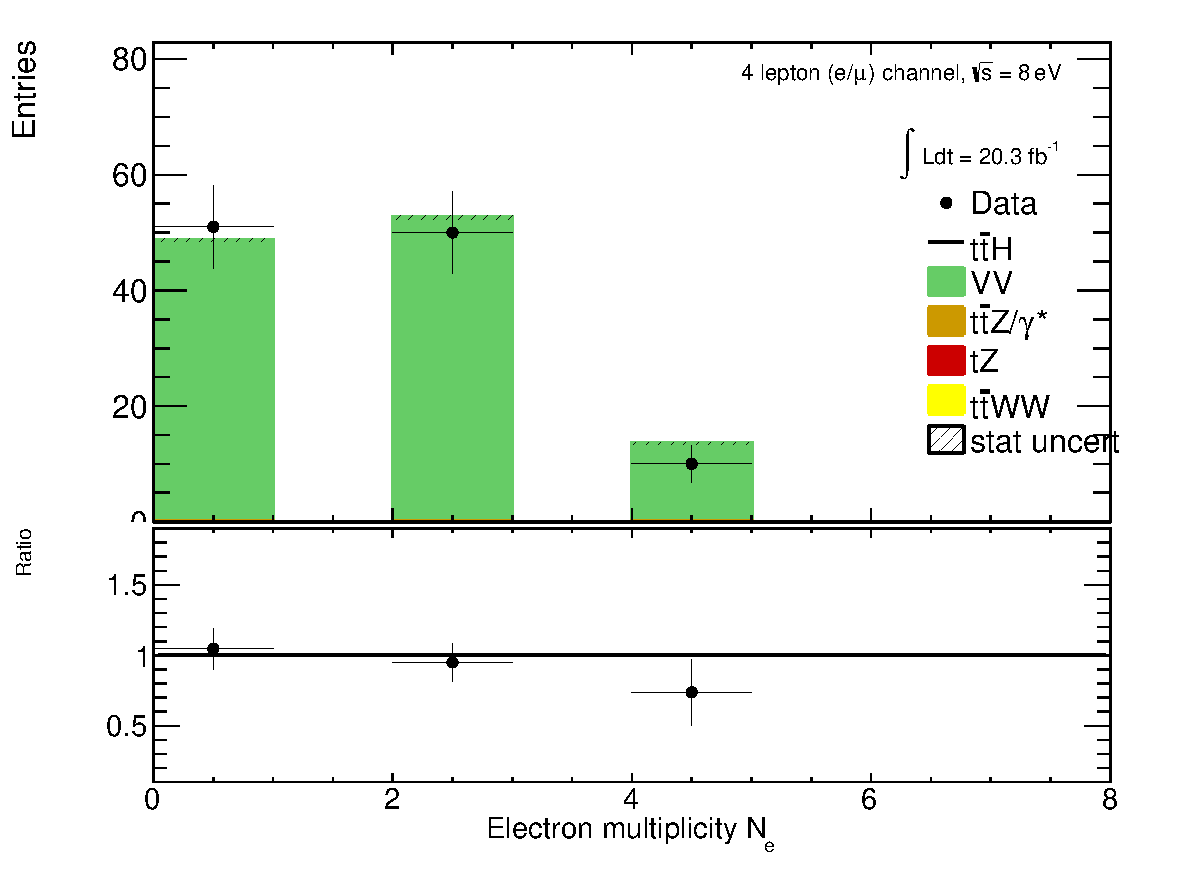
\includegraphics[width=\textwidth]{figs/WZ/plotCand_4lep_ZZ_CR_NElec}
  \end{minipage}\hfill
  \begin{minipage}[h]{0.5\textwidth}
    \centering 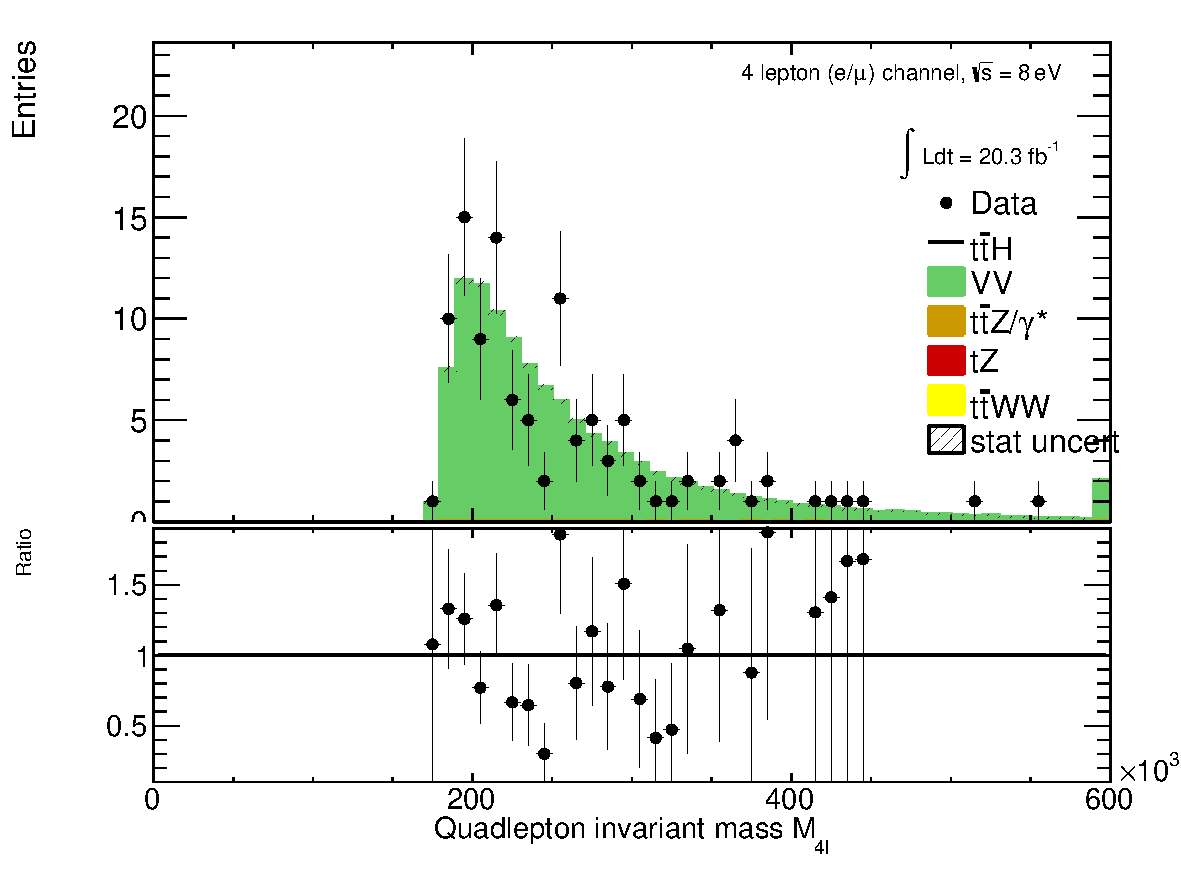
\includegraphics[width=\textwidth]{figs/WZ/plotCand_4lep_ZZ_CR_Mllll}
  \end{minipage}\hfill
  \begin{minipage}[h]{0.5\textwidth}
    \centering 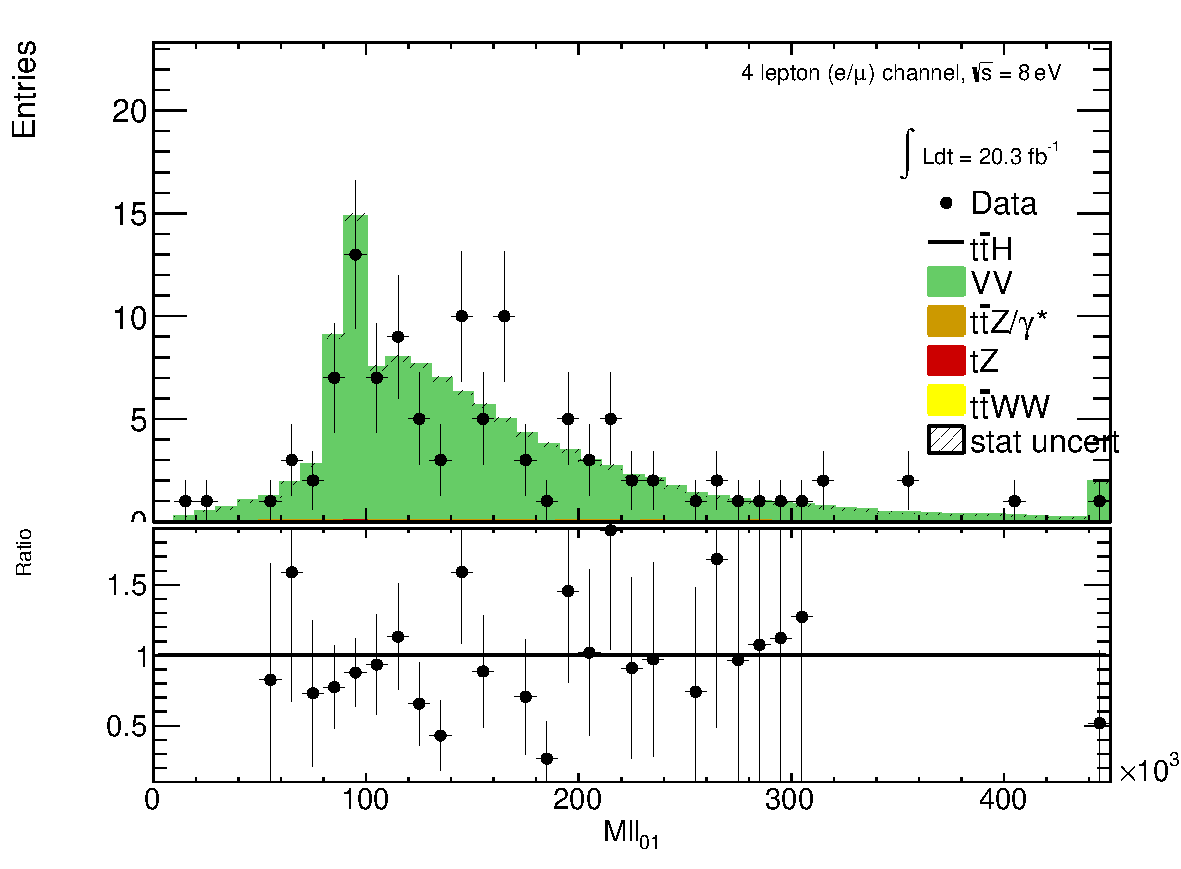
\includegraphics[width=\textwidth]{figs/WZ/plotCand_4lep_ZZ_CR_Mll01}
  \end{minipage}\hfill

  \caption{Jet-inclusive 4-lepton $ZZ$ validation region using the \tth\ lepton identification and momentum cuts }
  \label{figure:background_zz_incl}
\end{figure}


\begin{figure}[htbp]
  \begin{minipage}[h]{0.5\textwidth}
    \centering 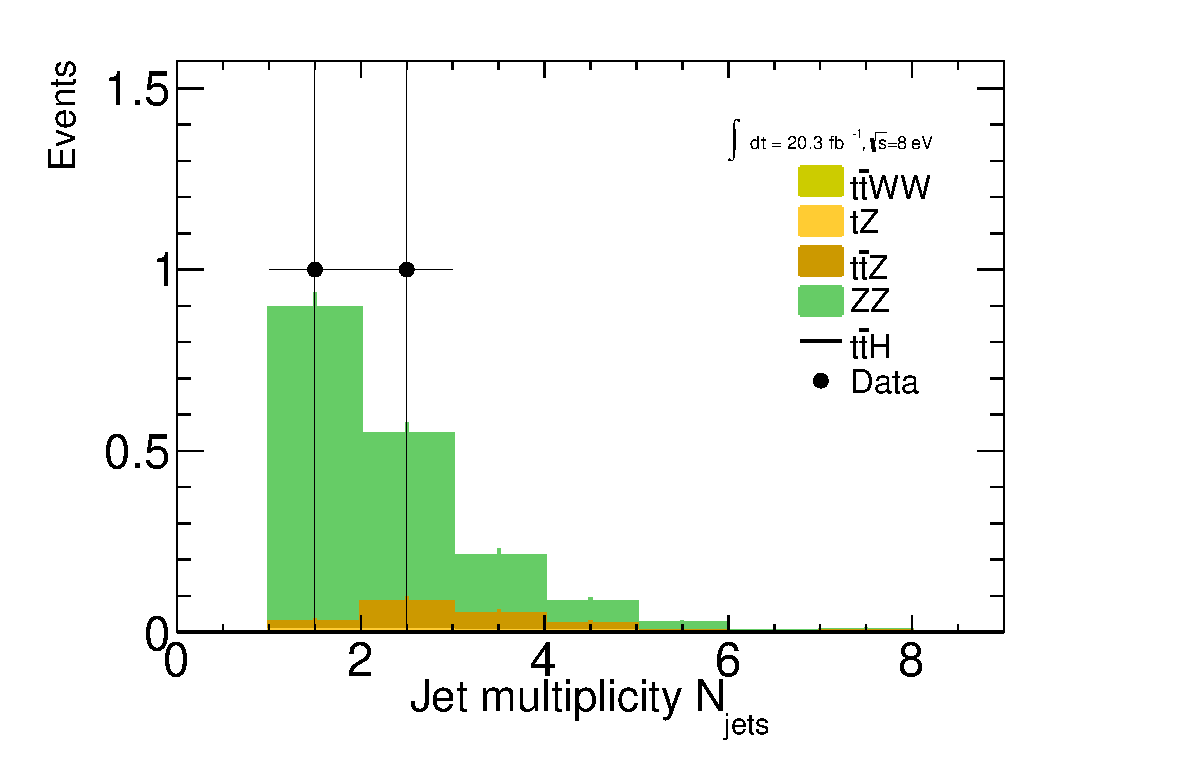
\includegraphics[width=\textwidth]{figs/WZ/zz_b_NJet}
  \end{minipage}\hfill
  \begin{minipage}[h]{0.5\textwidth}
    \centering 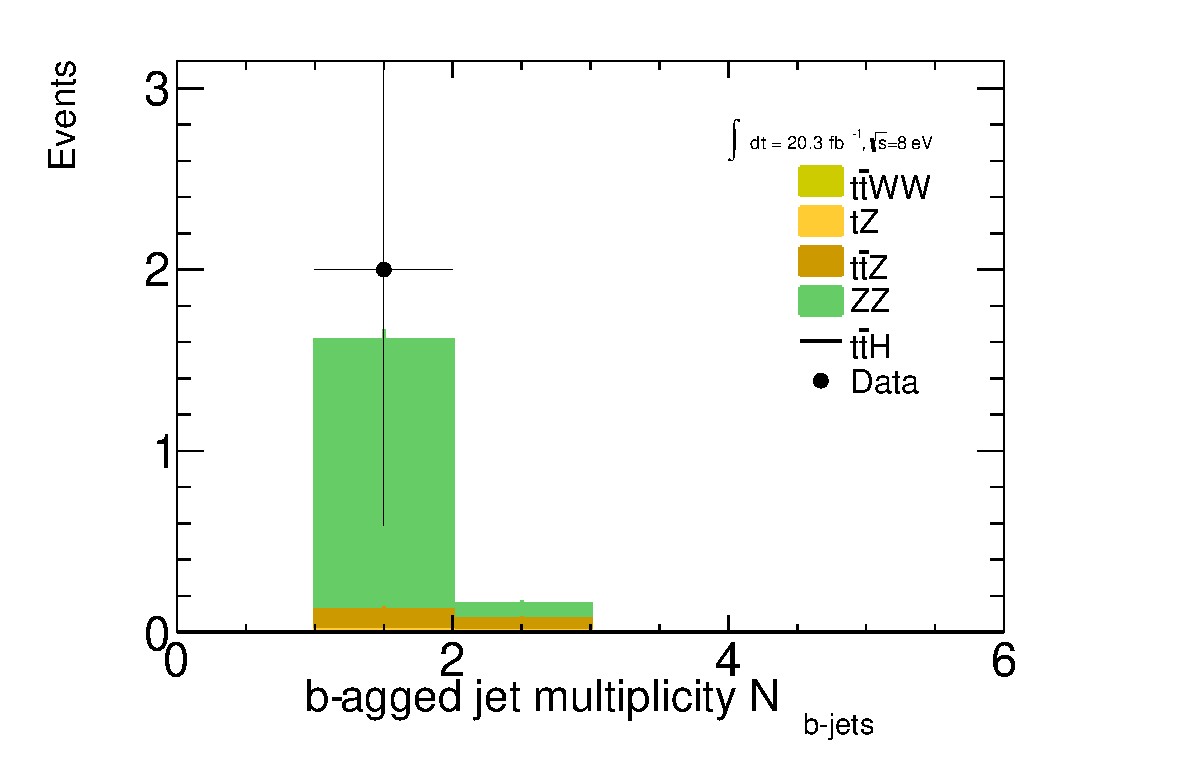
\includegraphics[width=\textwidth]{figs/WZ/zz_b_NJetBTag}
  \end{minipage}\hfill
        \caption{$ZZ+b$ validation region using the \tth\ lepton identification and momentum cuts }
        \label{figure:background_zz_z_b}
\end{figure}
 
Based on the study of the $ZZ$ and $ZZ+b$ validation regions and the overall agreement noted with the $Z+b$ analysis, we expect a similar error to \WZ\ to be appropriate in the $ZZ$ case.  A truth origin study is undertaken in MC to demonstrate a similar b-jet origin to the $W^{\pm}Z$ case. The true origin of the leading (highest energy) b-tagged jet is shown in Table \ref{table:zz_truth} for the 4-lepton signal region as well as the $ZZ+b$ validation region described above divided into jet bins. As it was in the $W^{\pm}Z$ case above, the true origin of the b-jet in $ZZ+b$ is dominated by c and b. Taking this study in tandem with the results from the $W^{\pm}Z$ investigation, it is appropriate to take the central value of the $ZZ+b$ background contribution in the 4-lepton SR from MC and to assign an overall systematic of 50\% in order to account for the MC modeling limitations. 

\begin{table}[htbp]
\centering 
\begin{tabular}{|c|c|c|c|} 
  \hline
                 & Bottom      & Charm       & Light \\
  \hline
  $ZZ+b$ VR 1 Jet& 0.56 $\pm$ 0.03 & 0.24 $\pm$ 0.01 & 0.20 $\pm$ 0.01 \\ 
  $ZZ+b$ VR 2 Jet& 0.52 $\pm$ 0.05 & 0.25 $\pm$ 0.02 & 0.23 $\pm$ 0.02 \\ 
  $ZZ+b$ VR 3 Jet& 0.53 $\pm$ 0.11 & 0.25 $\pm$ 0.08 & 0.22 $\pm$ 0.07 \\
  4$l$ SR        & 0.34 $\pm$ 0.15 & 0.42 $\pm$ 0.16 & 0.24 $\pm$ 0.10 \\
  \hline 
\end{tabular}
\caption{Truth origin of highest energy b-tagged jet in the $ZZ+b$ VR and 4$l$ SR} 
\label{table:zz_truth}
\end{table} 


\section{Charge-Misidentification Background }
\label{section:qmis} 
Charge-misidentification contributes to the background for 2$\ell$ SS case and only for flavor channels, which include electrons. The same-sign requirement is essential in removing large SM opposite sign-backgrounds, but because of their size even small charge misidentification rates result in contamination in same-sign regions. For the 2$\ell$ SS signal regions, charge-misidentification background arise primarily from \ttbar\ di-lepton events with a smaller contribution from leptonic $Z$ decays. 

In general, charge-misidentification can arise in two ways. The first occurs for ultra-high energy electrons and muons, which leave tracks in the detector that are too straight for the fit to determine the direction of curvature with high confidence. This type of charge misidentification is not a concern to the \tth\ multi-lepton analysis, as most of the leptons have transverse momentum $<$ 150 GeV. The second source of charge misidentification is from 'tridents', which only occurs for electrons, because their low mass allows for high rate bremsstrahlung in the detector material. In some cases, after an electron releases a photon through bremsstrahlung, the photon may convert nearby resulting in three electron tracks. The reconstruction algorithms may sometimes match the wrong track to the calorimeter energy deposit, resulting in a possible charge misidentification. As discussed in the selection, tight track-cluster geometric and energy matching requirements are applied on the electron candidates to reduce the overall rate and the electron acceptance is narrowed to ($|\eta| < 1.37$), since most of the material is concentrated more forward in the detector. 

We estimate the contribution of charge-misidentification events in our 2$\ell$ SS signal regions and relevant control regions by applying a weight per electron in the OS region with otherwise identical cuts. The weight is related to the charge-misidentification rates. We measure these rates using a likelihood method in the OS and SS $Z\rightarrow ee$ control region in data. The rate measured from these control regions is binned in electron \pt\ and $\eta$, to account for dependencies in these variables. The method, validations and associated errors are discussed in detail in the following sub-sections.


\subsection{Likelihood Method}

The number of reconstructed same-sign ($N_{ss}$) $Z\rightarrow ee$ events is related to total number of produced $Z\rightarrow ee$ ($N$) through factors related to the charge misidentification rate, $\epsilon$: 

\begin{equation}
N^{ij}_{ss} = N^{ij}(\epsilon_i + \epsilon_j - 2\epsilon_j\epsilon_i)
\end{equation}
where $\epsilon_i$ and $\epsilon_j$ are the charge misidentification rates for each electron separately. If we drop terms quardratic in $\epsilon$, we have:
\begin{equation}
N^{ij}_{ss}=N^{ij}(\epsilon_i+\epsilon_j).
\end{equation}
Although it is impossible to know event-by-event which electron's charge was misidentified, we can use a likelihood method over the whole $Z$ sample to measure how $\epsilon$ depends on the electron \pt\ and $|\eta|$. As illustration, we first consider the case, where $\epsilon$ depends on only one variable, $|\eta|$, and then generalize to the two-dimensional case of $|\eta|$ vs \pt. 

$N^{ij}_{ss}$ is described by a Poisson distribution:
\begin{equation}
f(k,\lambda)=\frac{\lambda^k e^{-\lambda}}{k!},
\end{equation}
where $k$ is the observed number of occurrences of the event, i.e. $k=N^{ij}_{ss}$, and $\lambda$ is the expected number,  i.e. $\lambda=N^{ij}(\epsilon_i+\epsilon_j)$. Thus, the probability for an observed number of same-sign $Z$ events given the sample size and charge misidentification rates is expressed by:
\begin{equation}
P(N^{ij}_{ss}|N^{ij},\epsilon_i,\epsilon_j)=\frac{[N^{ij}(\epsilon_i+\epsilon_j)]^{N_{ss}^{ij}}e^{-N^{ij}(\epsilon_i+\epsilon_j)}}{N^{ij}_{ss}!}.
\end{equation}
The likelihood $L$ for all the events is obtained by evaluating all the $|\eta|$ combinations:
\begin{equation}
L(\epsilon|N_{ss},N)=\prod_{i,j}\frac{[N^{ij}(\epsilon_i+\epsilon_j)]^{N_{ss}^{ij}}e^{-N^{ij}(\epsilon_i+\epsilon_j)}}{N^{ij}_{ss}!}.
\end{equation}
In this process, the $-\ln L$ is used in order to simplify and make easier the minimization. Terms which do not depend on the rates $\epsilon_i$ and $\epsilon_j$ are removed in this step. This way, the final function to minimize is given by the following expression:
\begin{equation}
\label{eq:like}
-\ln L(\epsilon|N_{ss},N)\approx \sum_{i,j}\ln[N^{ij}(\epsilon_i+\epsilon_j)]N^{ij}_{ss}-N^{ij}(\epsilon_i+\epsilon_j).
\end{equation}
The likelihood can be easily extended to depend on the charge misidentification rates as a function of two parameters. The probability to find a same-sign event given the rates for each electron is ($\epsilon_{i,k}+\epsilon_{j,l}$), where the two indices represent binned $|\eta|$- and $p_{\rm T}$-dependence. Thus, the Eq.~\ref{eq:like} transforms into
\begin{equation}
-\ln L(\epsilon|N_{ss},N)\approx \sum_{i,j,k,l}\ln[N^{ij,kl}(\epsilon_{i,k}+\epsilon_{j,l})]N^{ij,kl}_{ss}-N^{ij,kl}(\epsilon_{i,k}+\epsilon_{j,l}).
\end{equation}   

We use events selected within the $Z$ peak using the \tth\ electron object cuts. The events are stored in two matrices: one for the same-sign events $N^{ij,kl}_{ss}$,  and the other one for all events $N^{ij,kl}$. Small backgrounds need to be subtracted. The background subtraction is done using a simple side-band method.  This method consists in dividing the $Z$ invariant mass in three regions, i.e. $A$, $B$ and $C$, where $B$ is the central region corresponding to the $Z$ peak. The number of events is counted in the regions on the sides of the peak, i.e. $n_A$ and $n_C$, and removed  from the total number of events in the peak region $B$, $n_B$. This way, the number of signal events $N_Z$ is given by

\begin{equation}
N_Z=n_B-\frac{n_A+n_C}{2}.
\end{equation}
  
 Once the background has been subtracted, the likelihood is minimized for the 2D matrix of  $\epsilon$ bins. Knowing $\epsilon$ as a function of $|\eta|$ and \pt\ for any single electron, it is now possible to estimate the number of same-sign events from the number of opposite sign events in any sample:

\begin{itemize}
\item $N^{ss} = \frac{\epsilon_i +\epsilon_j -2\epsilon_i \epsilon_j}{1-\epsilon_i -\epsilon_j +2\epsilon_i \epsilon_j} N^{os}$ for $ee$ channels
\item $N^{ss} = \frac{\epsilon}{1-\epsilon} N^{os}$ for the $e\mu$ channels
\end{itemize}


\subsection{Results}

The charge misidentification rate is calculated in 7 $|\eta|$ bins [0.0, 0.6, 1.1, 1.37, 1.52, 1.7, 2.3, 2.47] by 4 \pt bins\ [15, 60, 90, 130, 1000] GeV. For \pt\ bins above 130 GeV, the $Z$ dataset becomes too small and the rates are calculated using \ttbar\ MC, scaled by the data-MC ratio of the rates in the lower \pt\ bins, [90-130] GeV. Figure \ref{figure:background_cf} shows the extracted rates in all bins.

\begin{figure}[ht!]
\centering
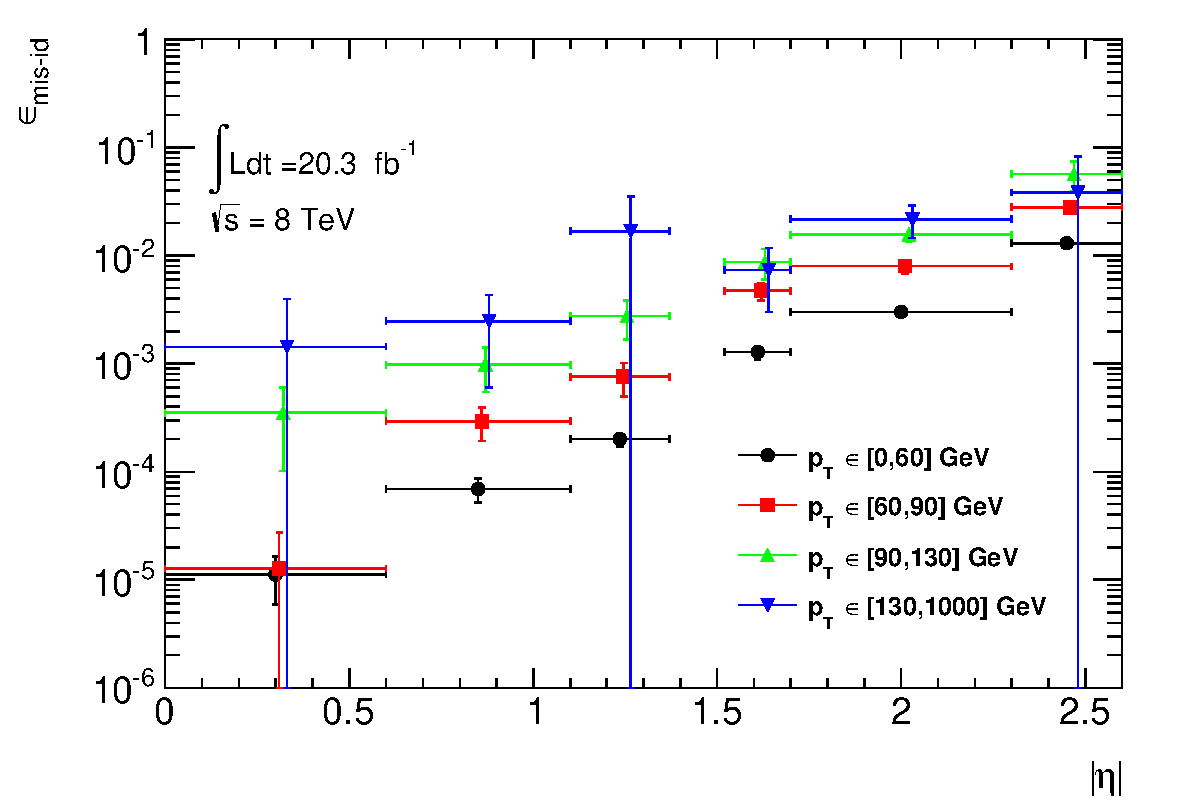
\includegraphics[width=0.7\textwidth]{figs/qmis/Rates2D}
  \caption{Electron charge misidentification rates  measured in data with the likelihood method  on $Z$ events (black points, red squares and blue triangles) as a function of $|\eta|$ and parametrized in $p_{\rm T}$. The full 2012 dataset has been used to estimate the rates below 130~GeV.   Above this value, the charge misidentification rates have been estimated by extrapolating the rates in the region where the $p_{\rm T}\in[90,130]$~GeV with a $p_{\rm T}$ dependent factor extracted from simulated $t\bar t$ events (green triangles). Statistical and systematic uncertainties  have been included in this plot. \label{figure:background_cf}}
\end{figure}


As a cross-check, we apply the full method to the $Z$ MC samples (extracting rates via a likelihood fit and applying them to opposite sign events) and compare to the MC predicted number of same-sign events. The invariant mass of the $Z$ from our charge misidentification and directly from the MC can be seen on Figure~\ref{figure:background_clMll}. In the simulated $Z$ samples, the number of same-sign $Z$ events is $5~049$ while the estimation is $5~031^{+375}_{-365}$.  The uncertainties combine both statistical systematic uncertainties, which are discussed in depth below. The validation gives compatible results within uncertainties. 
 
\begin{figure}[htb!]
\centering
\begin{minipage}[h]{0.5\textwidth}
    \centering 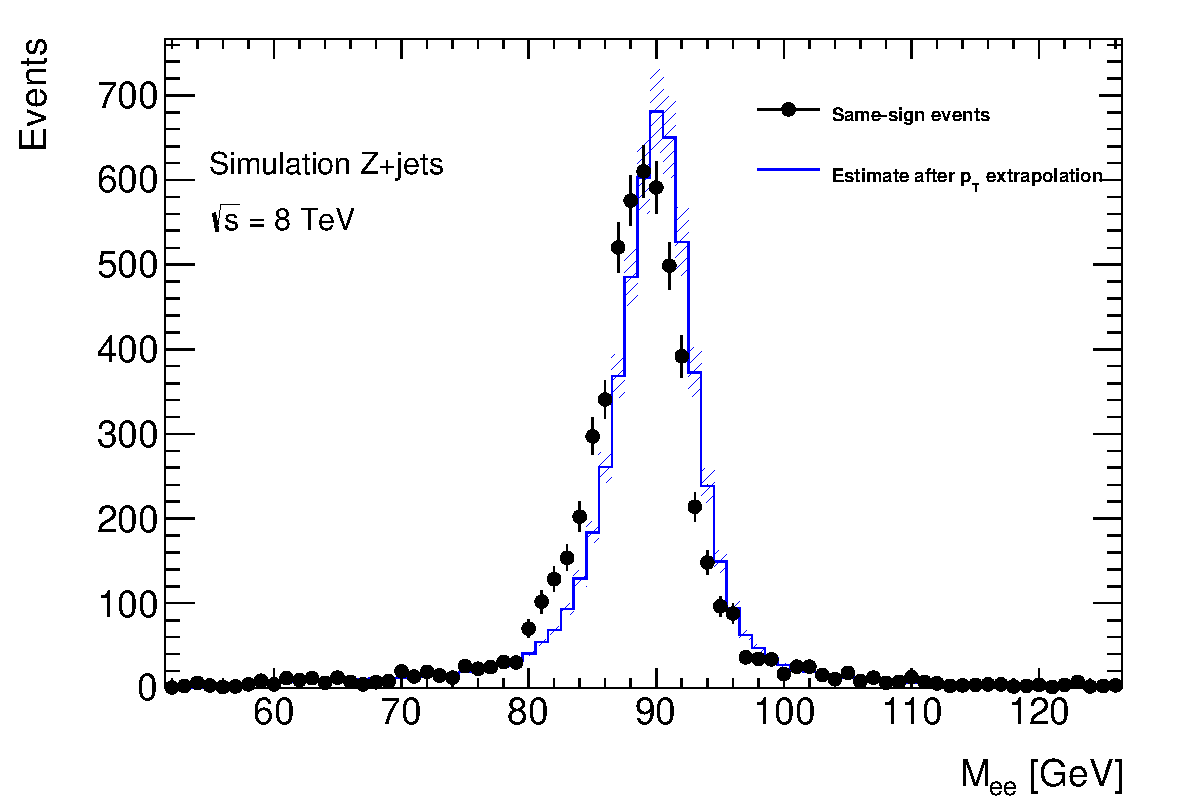
\includegraphics[width=\textwidth]{figs/qmis/ClosureMllMC}
\end{minipage}\hfill
\begin{minipage}[h]{0.5\textwidth}
    \centering 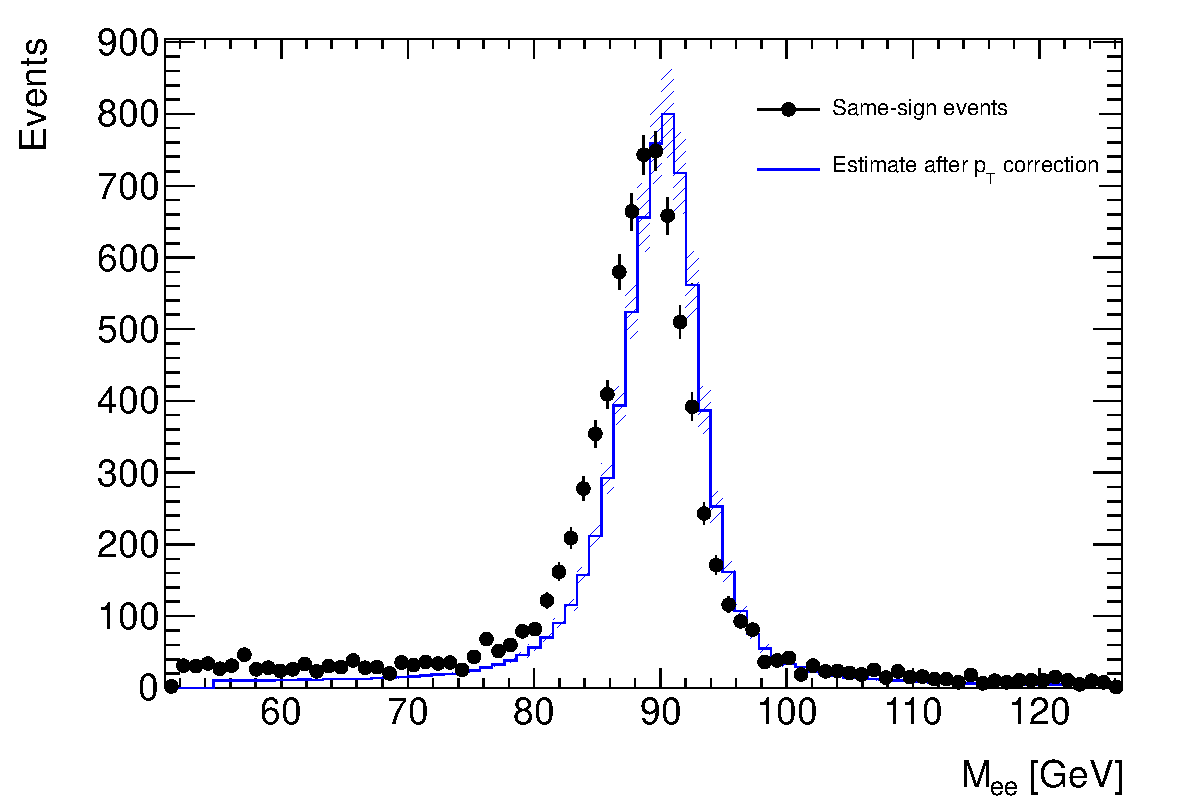
\includegraphics[width=\textwidth]{figs/qmis/ClosureMlldata}
\end{minipage}\hfill
  \caption{Closure test on simulated $Z\rightarrow e^+e^-$ events (a)   and data (b). 
      The black circles show the distribution of same-sign events while the blue histograms
      show the distribution of the re-weighted opposite-sign events together with the statistical and systematic uncertainties. The distributions are not
    expected to overlay exactly, due to the loss of energy of the trident electrons for the
    same-sign peak. \label{figure:background_clMll}}
\end{figure}


\subsection{Systematic and Statistical Uncertainties}

Statistical uncertainties dominate the combined uncertainty on the charge misidentification estimate. The statistical uncertainties come primarily from the size of the $Z$ same-sign sample in data and are especially large for central, material-poor regions where the charge misidentification rate is extremely low. Additional systematic uncertainties are included for a comparison between the positron and electron rate, the per-bin MC closure test discussed above, and for the effect of varying the invariant mass window used for the background subtraction for three different cases. Figure \ref{figure:background_qmissyst} shows the relative uncertainties for all rate bins.



 \begin{figure}[htp!] 
\centering
\setlength{\fboxrule}{0 pt}
\fbox{  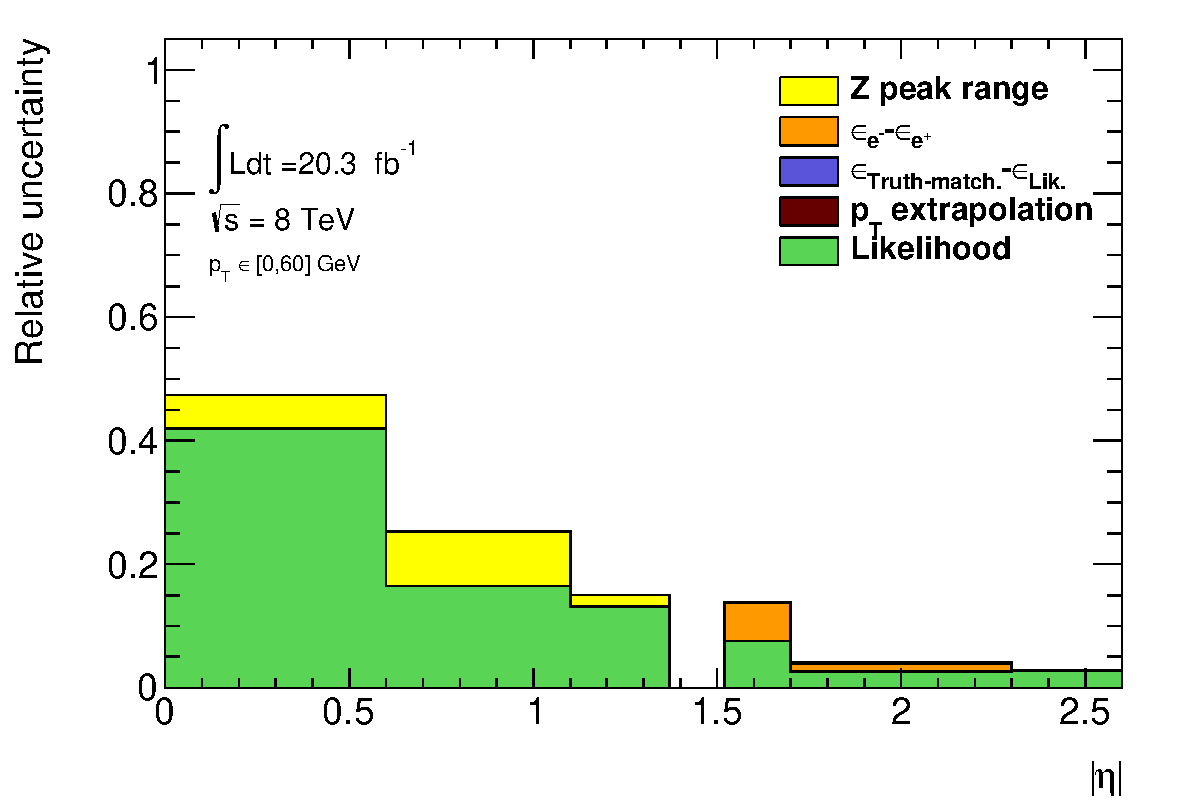
\includegraphics[width=0.48\textwidth]{figs/qmis/Syst1}}% \hspace{2cm}%
\fbox{  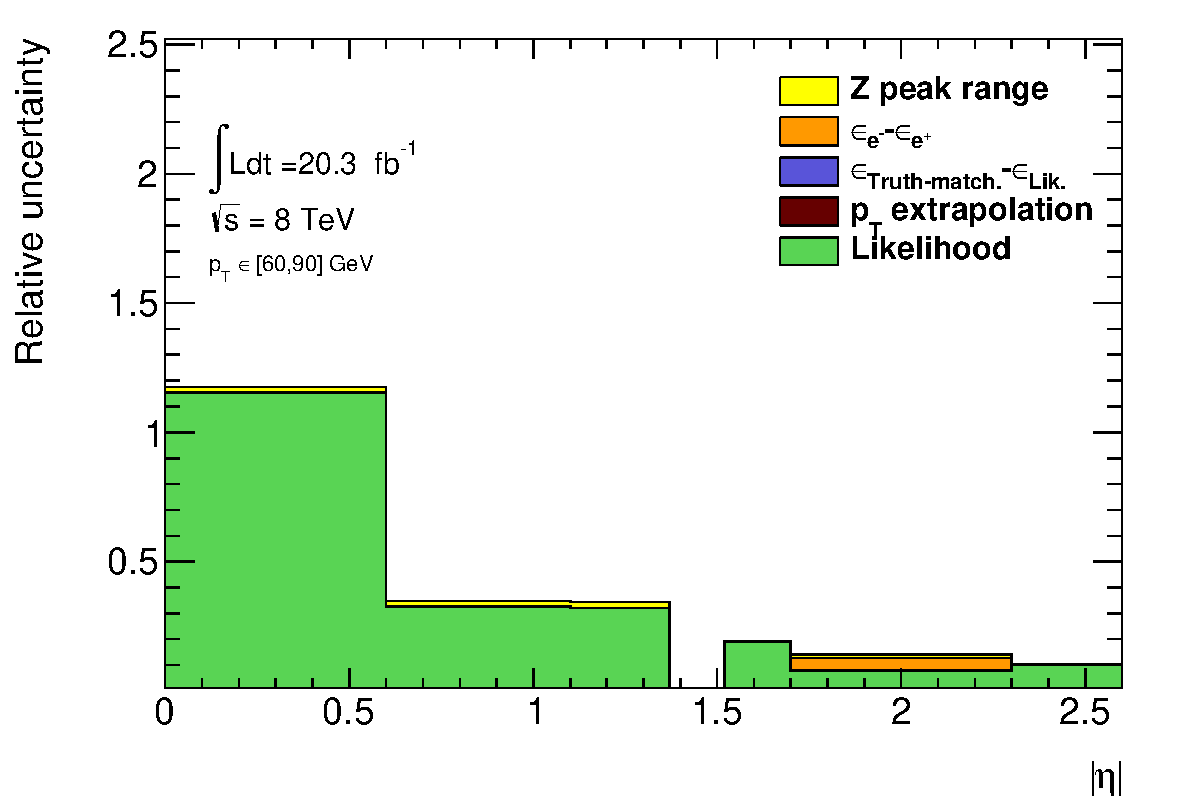
\includegraphics[width=0.48\textwidth]{figs/qmis/Syst2}}% 

\fbox{  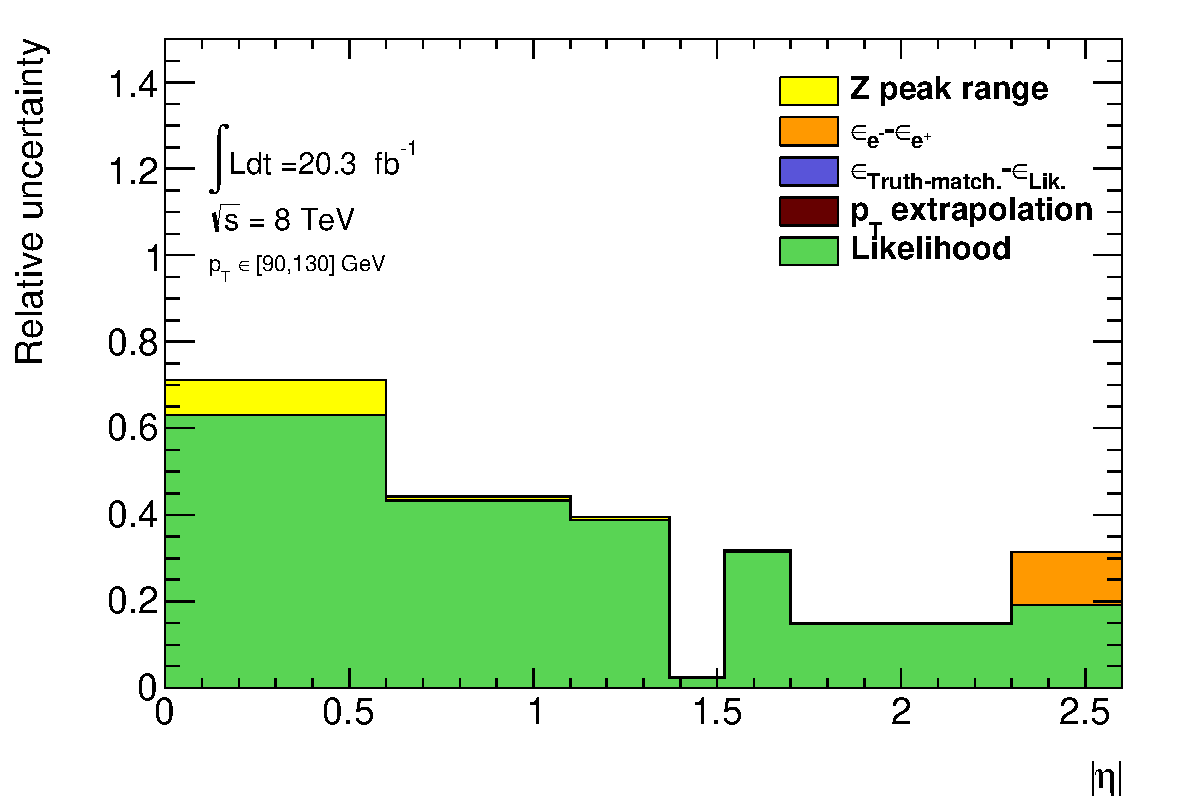
\includegraphics[width=0.48\textwidth]{figs/qmis/Syst3}}% hspace{2cm}%
\fbox{  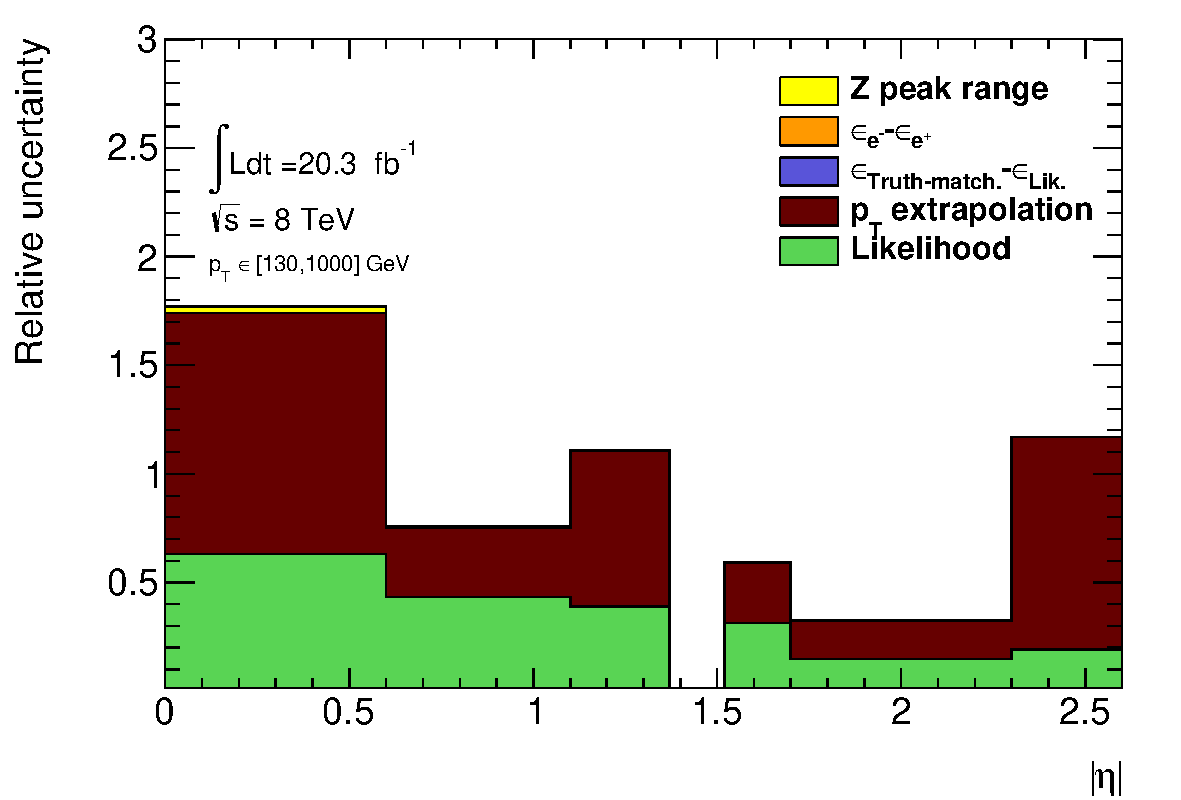
\includegraphics[width=0.48\textwidth]{figs/qmis/Syst4}}% 
\caption{Relative systematic uncertainty contributions on the
      charge misidentification rate, for different bins in $p_{\rm T}$ and 
      $|\eta|$.}\label{figure:background_qmissyst}
 \end{figure}

We apply the rates to estimate the charge misidentification background in the 2$\ell$ SS signal regions, and find  $\sim$ 25\% contamination in the \ee regions and a $\sim$ 10\% contribution to the \emu regions with a 10\% systematic error overall. The low overall error can be attributed to the fact that the statistical error is lowest where the bulk of charge misidentifications occur. The charge flip contribution measured in the signal regions from this method is detailed in Table~\ref{table:background_summary}. 


\section{Fake Lepton Backgrounds}
\label{section:fakes}
Fake Leptons, from the misidentification of jets as either electrons or muons, primarily arise from \ttbar\ and single top processes in the 2$\ell$ SS, 3$\ell$ and 4$\ell$ channels. Smaller contributions come from $Z$+jet events. Fake backgrounds are sub-dominant but important in the 2$\ell$ SS and 3$\ell$ channels. They are extremely small in the 4$\ell$ channels. Truth studies suggest that these misidentified leptons arise overwhelmingly from b-quark initiated jets. The general method for estimating fakes in all channels is to define a reversed object selection control region (usually isolation) for each lepton flavor with otherwise identical signal region selection ($N^e_{CR}$, $N^{\mu}_{CR}$). This region is fake-dominated. The total number of fake events in these regions are then scaled by transfer factors ($\theta$) to estimate the number of fake events of the appropriate flavor in the signal region. The simple formula for determining fakes is defined in Equation \ref{equation:background_total}.    


\begin{equation}
N_{fake} = \theta_e \cdot N^e_{CR} + \theta_{\mu} \cdot N^{\mu}_{CR}   
\label{equation:background_total}
\end{equation}

This approach factorizes the background model into two separate measurements. $N_{CR}$ is sensitive the overall \ttbar\ production rate, especially in the presence of additional jets from QCD ratio, as well as the object-level misidentification of a jet as a lepton. The transfer factors are sensitive to only the object level properties of the misidentified jet, and in particular only the variables which are reversed in the anti-tight identification. 

The transfer factors are obtained obtained in a different way for each channel, due to unique issues with statistics and contamination, but each method relies heavily on the data-based control regions with fewer jets. Figure \ref{figure:background_njetr} shows a truth study of the stability of the transfer factor for the 2$\ell$ SS and 3$\ell$ cases as a function of the number of jets in the event for events with one-b-tagged jet. This suggest that the regions with fewer jets are a good model of the fakes in the signal regions with more jets and is expected because of the homogeneity of origin of the fakes across all jet bins.  

The details of the methods for each channel are discussed in depth in the following sections. For all methods, the overall systematic uncertainty on the normalization of the fake estimate is in the range 30\%-50\% and arise primarily from statistics and the closure on assumptions used to obtain the transfer factor.

\begin{figure}[htbp]
\begin{minipage}[h]{0.5\textwidth}
    \centering 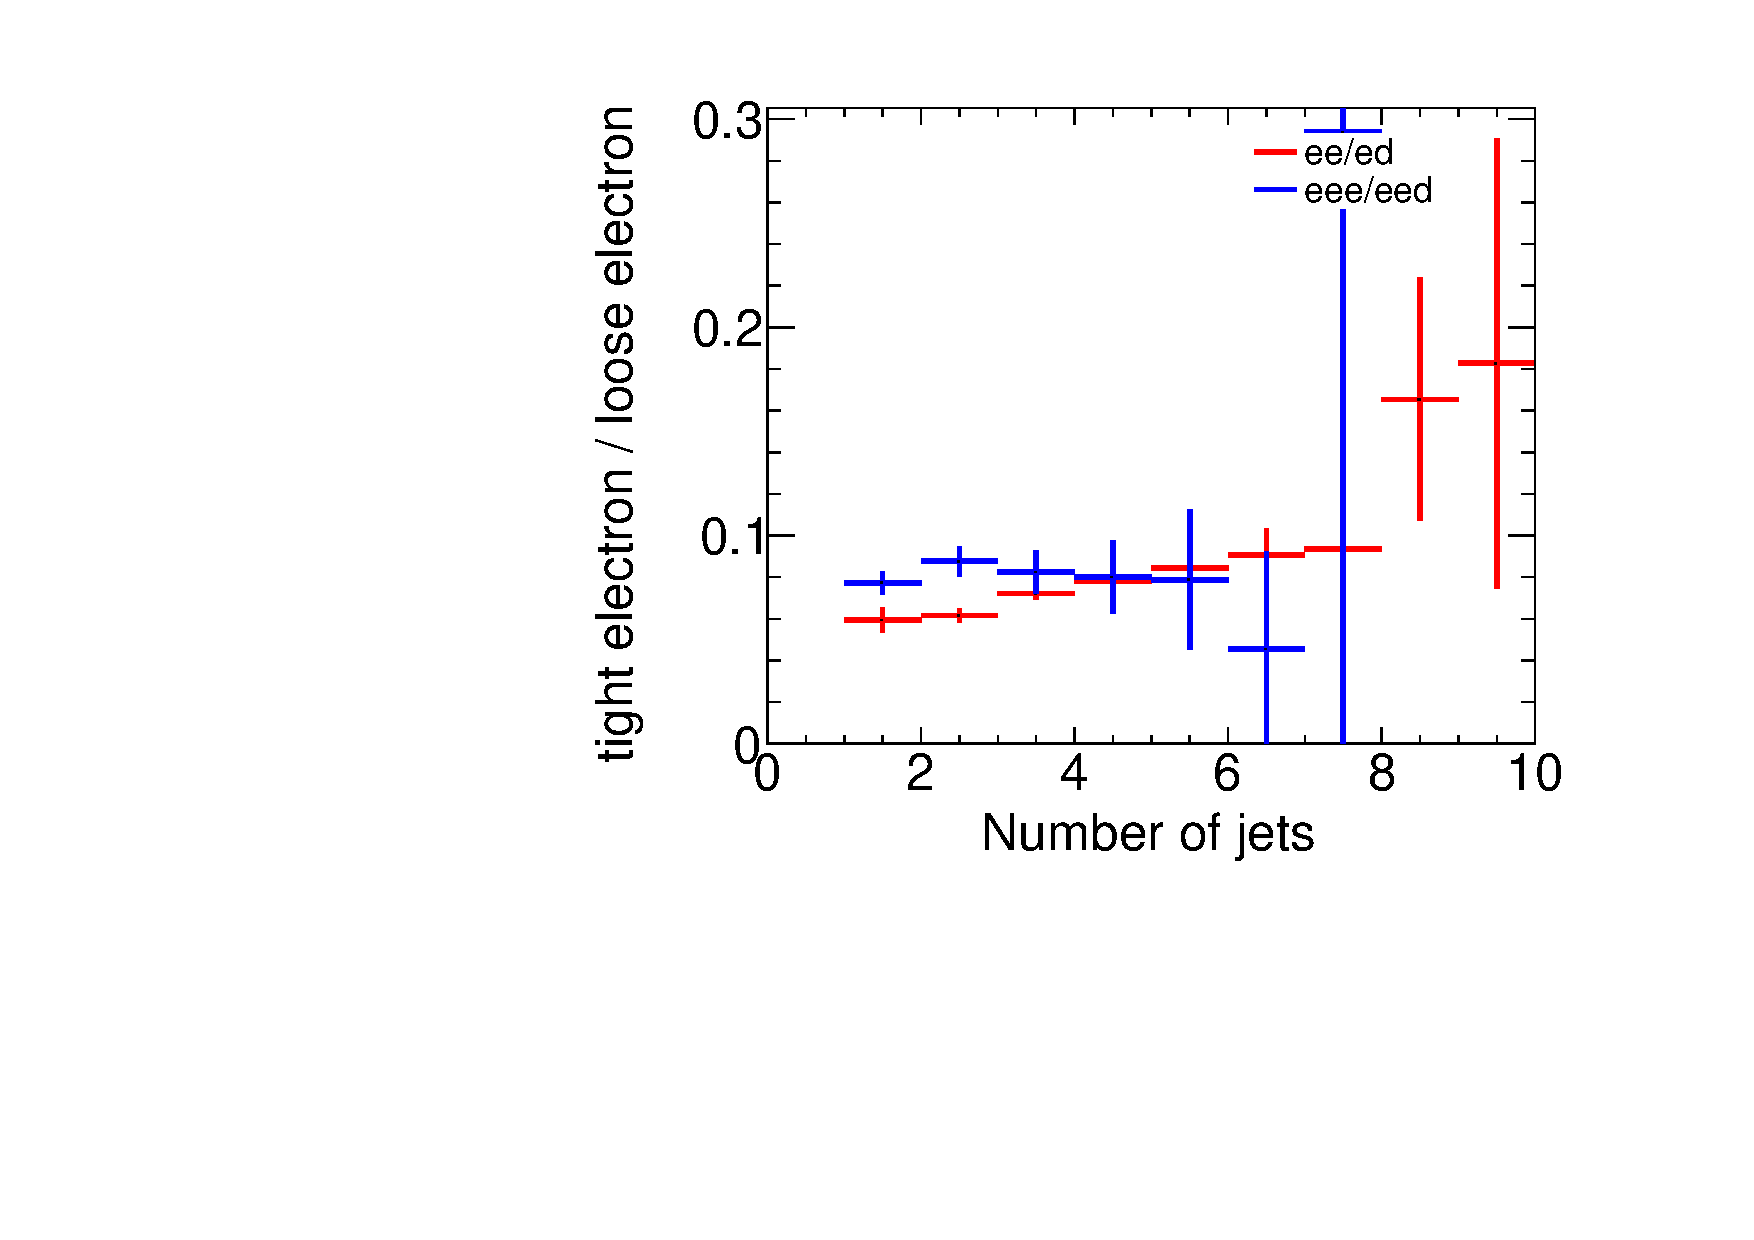
\includegraphics[width=\textwidth]{figs/fake/compare_2e_3e_NJet_ratios}
\end{minipage}\hfill
\begin{minipage}[h]{0.5\textwidth}
    \centering 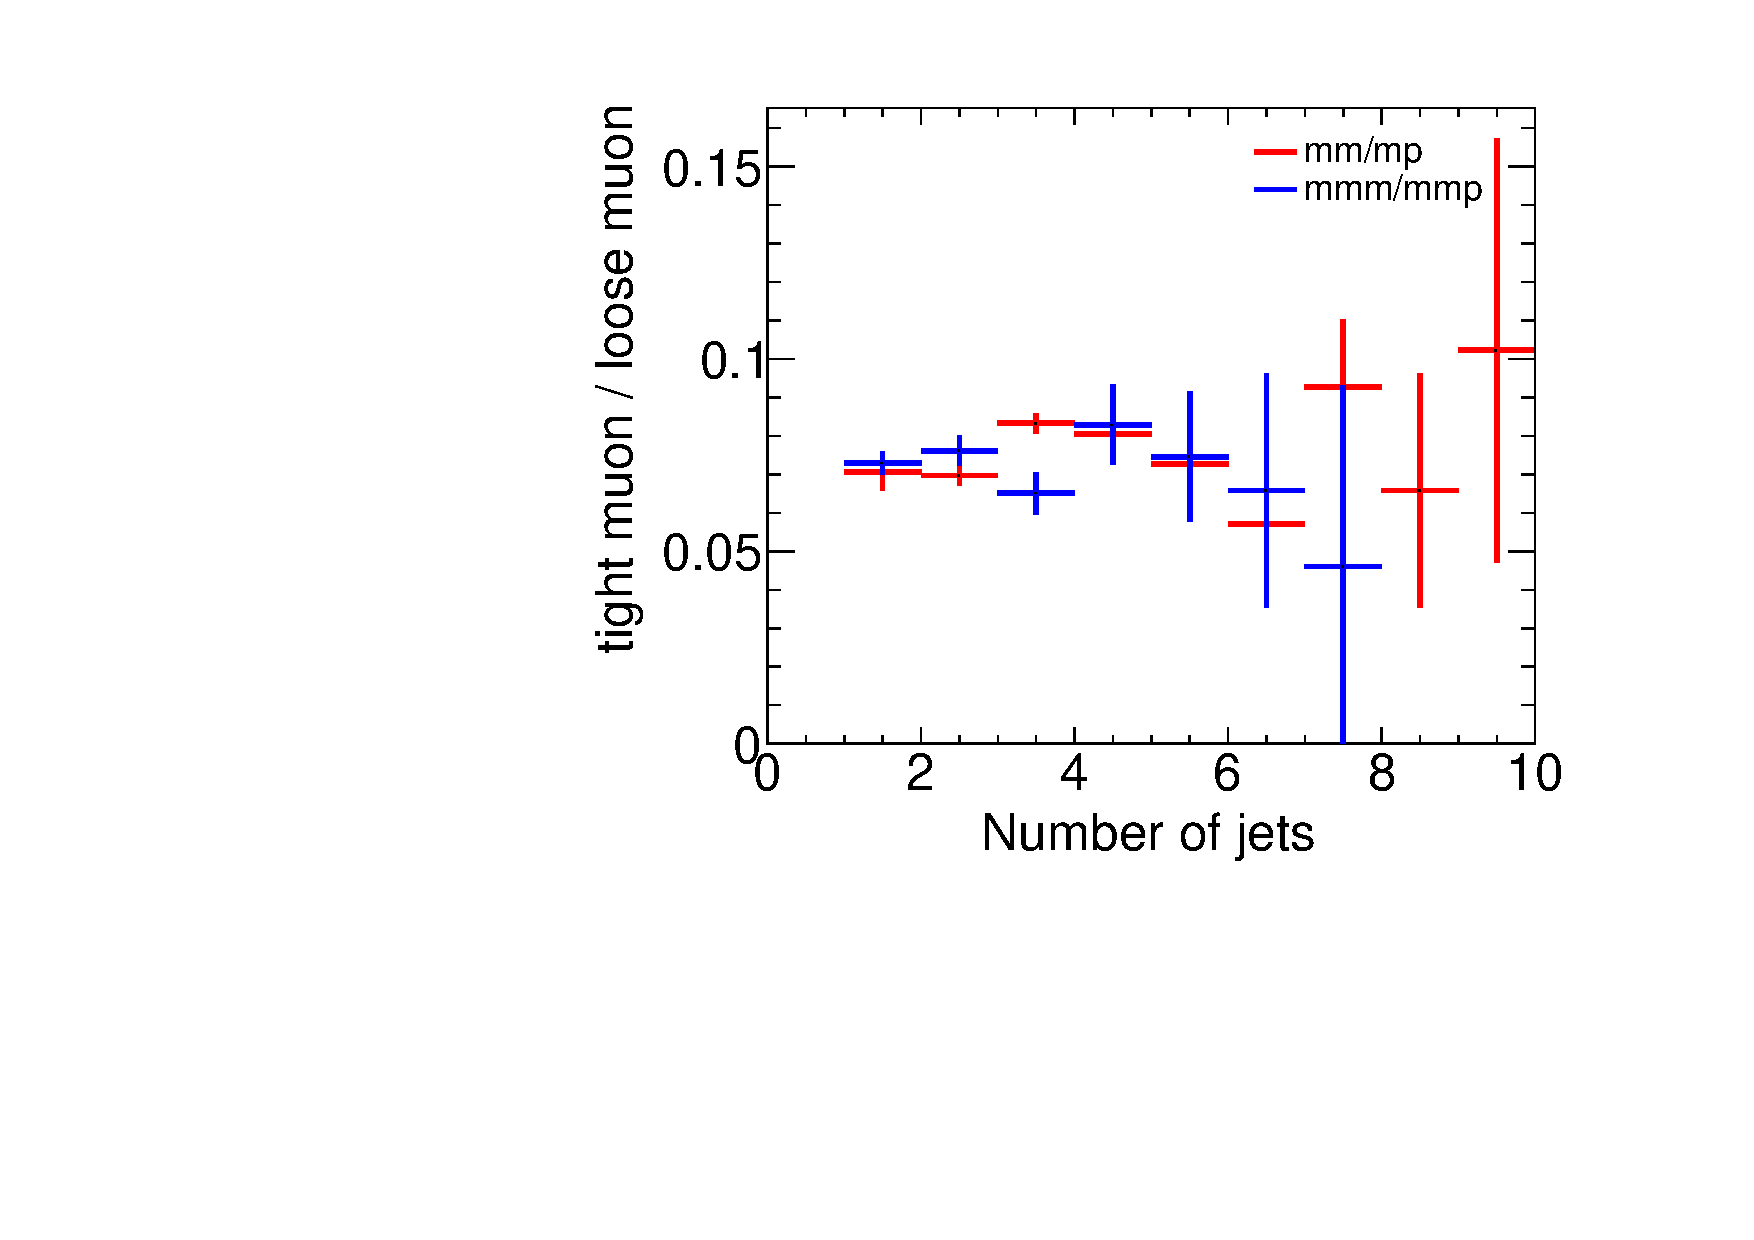
\includegraphics[width=\textwidth]{figs/fake/compare_2m_3m_NJet_ratios}
\end{minipage}\hfill
\caption{Ratios of regions with tight and anti-tight leptons in 2-lepton and 3-lepton channels from \ttbar\ MC. These ratios are the MC calculated transfer factors for each region, i.e. $\theta_e$ = $eee/eed$, $ee/ed$ and $\theta_{\mu}$ =$mmp/mmm$, $mm/mp$, where 'd' refers to anti-tight electrons and 'p' referes to anti-tight muons. The transfer factors are seen to be similar in the 2$\ell$ and 3$\ell$ cases and stable as a function of the number of jets}
\label{figure:background_njetr}
\end{figure}

Because these methods do not provide a per-object transfer-factor that depends on the properties of the faking object, we must use the MC to model the shapes of the fake kinematic distributions in the signal regions. This is not an essential issue, since the analysis only considers only the total number of events in each signal region in the final measurement of \tth\ production.

\subsection{2$\ell$ SS Fakes}
The 2$\ell$ SS fake method follows the procedure outlined in general above. We define anti-tight electron and muon control regions with reversed particle identification criteria for each signal region, including the 6 flavor and jet-counting sub regions. The anti-tight muon and electron criteria are provided below:
  
\begin{itemize}

\item \textbf{anti-tight electron (d):} fails the {\textsc verytight} likelihood operating point, but still passes the {\textsc veryloose} operating point. fails relative tracking and calorimeter isolation, $\rm E_{T}^{rel}>0.05$ and $\rm p_{T}^{rel}>0.05$.

\item \textbf{anti-tight muon (p):} 6 GeV $<$ \pt\ $<$ 10 GeV

\end{itemize}

The electron and muon transfer factors, $\theta_e$ and $\theta_{\mu}$, are calculated in the region with signal region selection but fewer jets, $NJet == 2$ or $NJet ==3$ and are defined as the ratio of the number of events for two fully identified leptons to the number of events with one fully identified lepton and one anti-identified lepton, after the prompt and charge misidentification backgrounds are subtracted. Only same-flavor channels are used to ensure that muon and electron transfer factors maybe estimated separately:
on every region, the prompt and charge-misidentification backgrounds are subtracted from the data. 

 \begin{equation}
 \theta_{e} = \frac{N_{ee}}{N_{ed}}= \frac{  N^{Data}_{ee} - N^{\rm
 Prompt~SS}_{ee} - N^{\rm QMisId}_{ee} }{ N_{ed}^{Data} - N^{\rm
 Prompt~SS}_{ed} - N^{\rm QMisId~MC}_{ed} } 
\end{equation}
\label{equation:ss_def_thee}


 \begin{equation}
 \theta_{\mu} = \frac{N_{\mu\mu}}{N_{\mu p}}= \frac{ N_{\mu\mu}^{Data} - N^{\rm
 Prompt~SS}_{\mu\mu}}{ N_{\mu p}^{Data} - N^{\rm
 Prompt~SS}_{\mu p} } 
\end{equation}
\label{equation:ss_def_thmm}

The 2,3 jet anti-tight regions used in obtaining the transfer factors are shown in Table~\ref{table:background_23jets} and the 4,5 jet
anti-tight regions, scaled by the transfer factors to get the fake estimates in the SR are shown in Figure \ref{figure:background_45jets}. 
The \ttbar\ and single top MC are included in the plots and tables for reference, although they are not used in the measurements. 

\begin{table}
  \begin{center}
\begin{tabular}{ c c }%% structure globale

\begin{tabular}{|c|c|}
\hline Process & N(events) \\ \hline
\multicolumn{2}{|c|}{$ed$ $\le 3$ jets} \\ \hline
$VV$  &    $7.13\pm0.63$ \\
$V\gamma$  &  $7.55\pm1.27$ \\
$t\bar{t}V, tV$     &    $6.68\pm0.18$ \\\hline
$V+jets$     &    $59.4\pm18.51$ \\
$t\bar{t},t+X$ &    $671.26\pm12.76$ \\
~$t\bar{t}$ prompts &    $32.97\pm 2.83$ \\\hline
Total MC & $752.0\pm22.5$ \\
Data & $967$ \\ \hline
Data fakes (Data - prompts) & $912.66$ \\ \hline\hline

\multicolumn{2}{|c|}{$ee$ $\le 3$ jets} \\ \hline
$VV$  &    $3.55\pm0.45$ \\
$V\gamma$  &  $1.43\pm0.70$ \\
$t\bar{t}V, tV$     &    $4.14\pm0.17$ \\\hline
$V+jets$     &    $8.3\pm8.8$ \\
$t\bar{t},t+X$ &    $11.65\pm1.67$ \\ \hline
Charge misID &    $ 8.54 \pm 0.23 $ \\\hline
Total MC & $28.52 \pm 8.96$  \\
Data & $32$ \\ \hline
Data fakes (Data - prompts) & $14.32$ \\ \hline\hline

\end{tabular}

&


\begin{tabular}{|c|c|}
\hline Process & N(events) \\ \hline

\multicolumn{2}{|c|}{$\mu p$ $\le 3$ jets} \\ \hline
$VV$  &    $1.14\pm1.99$ \\
$V\gamma$  &  $1.14\pm1.14$ \\
$t\bar{t}V, tV$     &    $0.642\pm0.060$ \\\hline
$V+jets$     &    $24.48\pm17.64$ \\
$t\bar{t},t+X$ &    $104.91\pm5.14$ \\\hline
Total MC & $171.38 \pm 18.89$ \\ 
Data & 141 \\ \hline
Data fakes (Data - prompts) & $138.08$ \\ \hline\hline

\multicolumn{2}{|c|}{$\mu\mu$ $\le 3$ jets} \\ \hline
$VV$  &    $3.55\pm0.42$ \\
$V\gamma$  &  $0$ \\
$t\bar{t}V, tV$ &    $9.37\pm0.26$ \\\hline
$V+jets$     &    $0.16 \pm 11.81$ \\ %% huge number of samples with 0 evts %% -> neglected
$t\bar{t},t+X$ &  $12.90\pm1.93$ \\\hline
Total MC & $27.18 \pm 11.98$ \\ 
Data & 47 \\ \hline
%%Data / MC & $1.18 \pm 0.17 $ \\ \hline
Data fakes (Data - prompts) & $34.08$ \\ \hline\hline

\end{tabular}


 \end{tabular}

\caption{Number of events of the main simulated background processes and of
  the data in the \ee and \mumu channels used for the measurement of
  $\theta_e$ and $\theta_\mu$. $VV$, $V\gamma$, $t\bar{t}V, tV$ and $t\bar{t}$~prompts
  (or charge misID) are the backgrounds which lead to prompt same-sign dileptons and are subtracted from
  the data to get a measured number of fakes. Uncertainties are
  statistical. The numbers labeled Data fakes are used to
  measure $\theta$. 
  \label{table:background_23jets}} 
\end{center} \end{table}
 

  % Figures
 \begin{figure}[htbp]

  \begin{minipage}[h]{0.5\textwidth}
    \centering 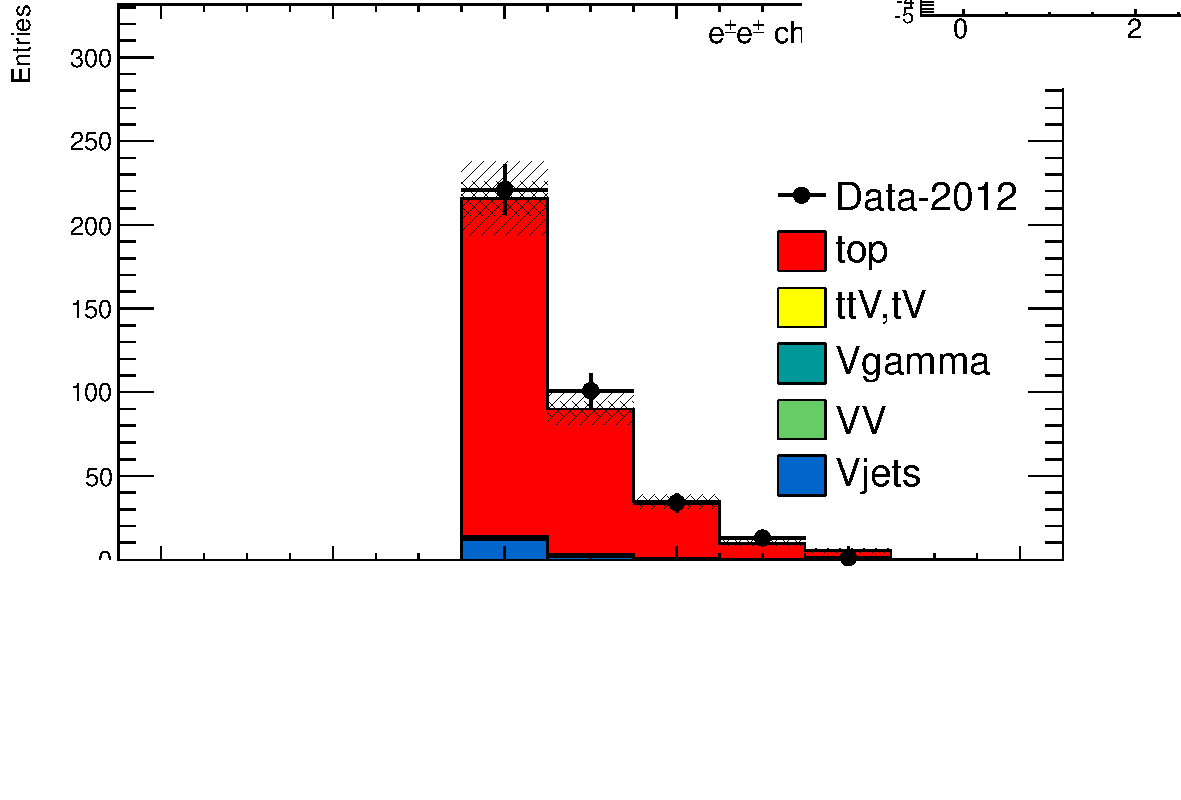
\includegraphics[width=\textwidth]{figs/fake/TaT-5jets-1b_nj_ee}
  \end{minipage}\hfill
  \begin{minipage}[h]{0.5\textwidth}
    \centering 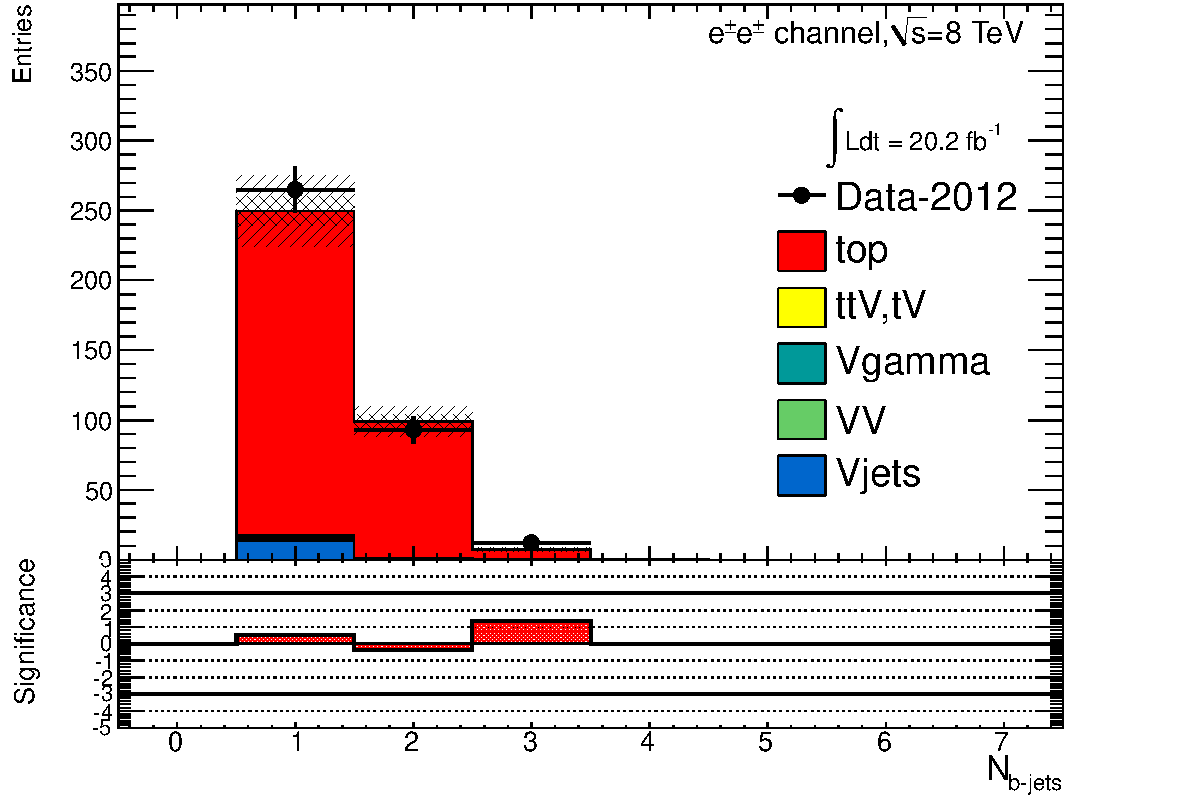
\includegraphics[width=\textwidth]{figs/fake/TaT-5jets-1b_nb_ee}
  \end{minipage}\hfill
  \begin{minipage}[h]{0.5\textwidth}
    \centering 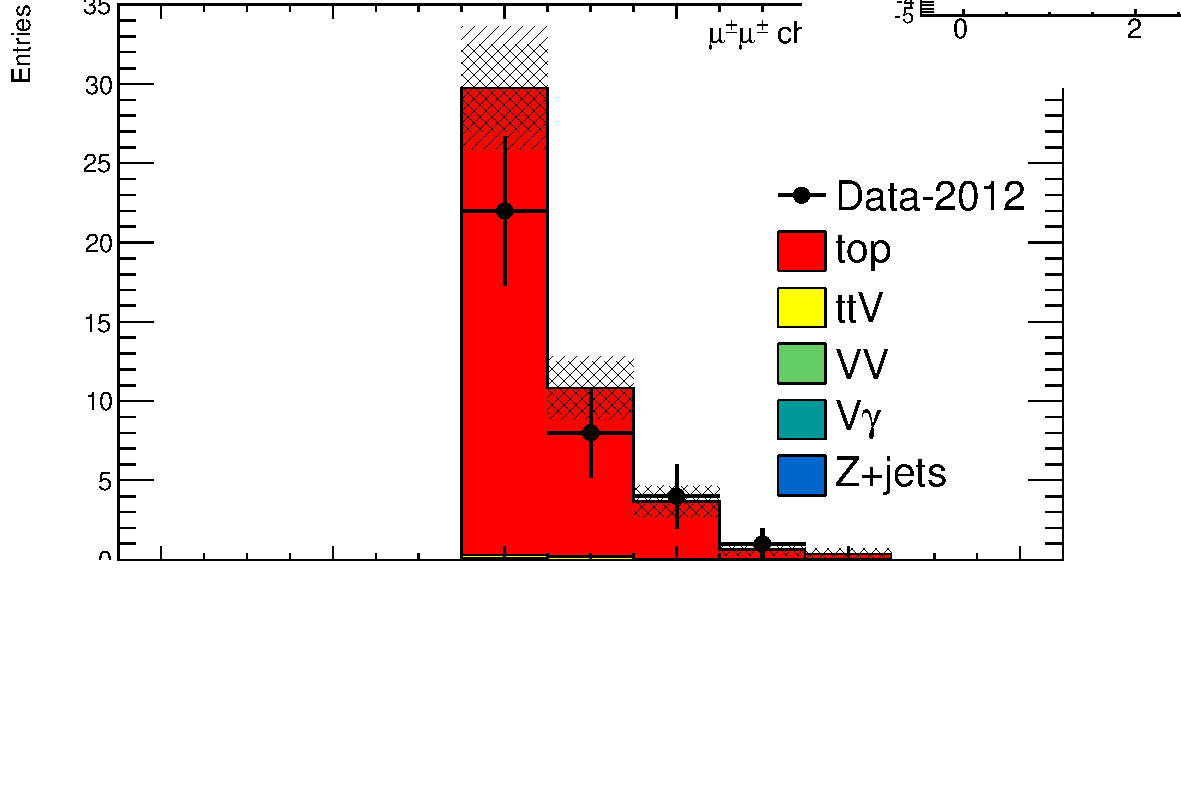
\includegraphics[width=\textwidth]{figs/fake/TaT-5jets-1b_nj_mm}
  \end{minipage}\hfill
  \begin{minipage}[h]{0.5\textwidth}
    \centering 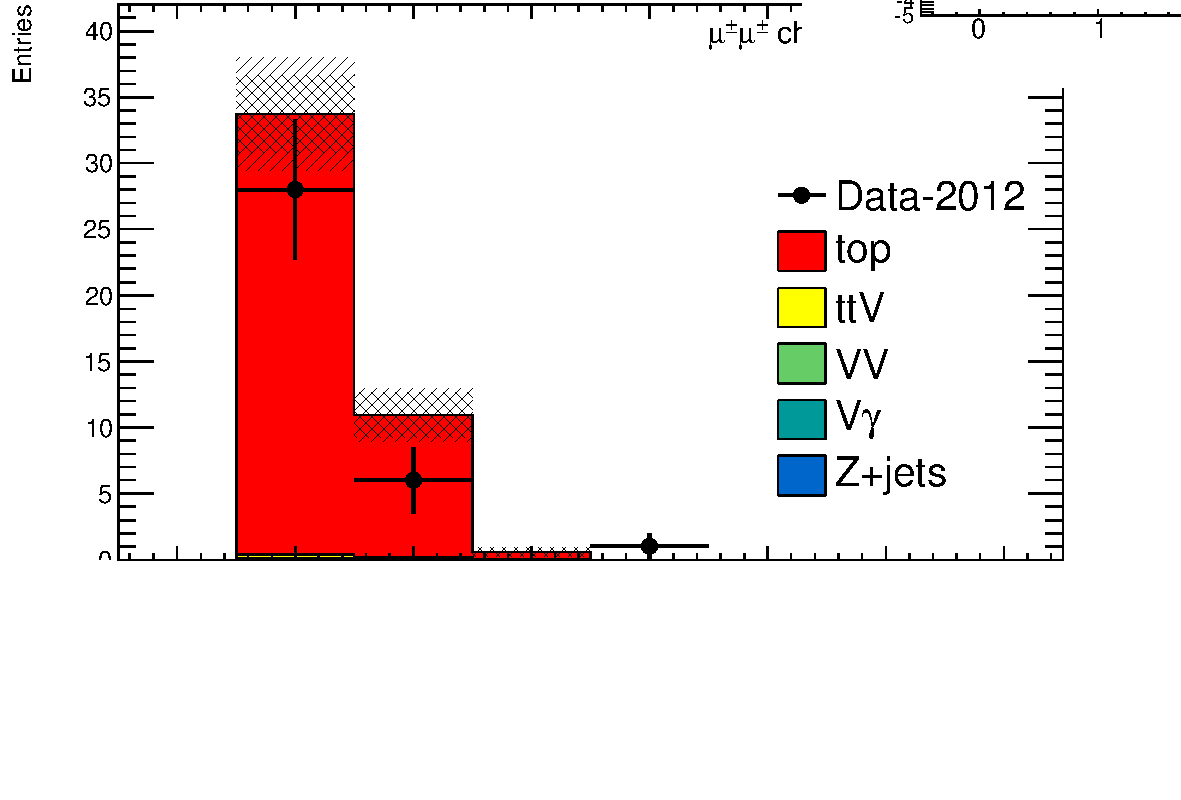
\includegraphics[width=\textwidth]{figs/fake/TaT-5jets-1b_nb_mm}
  \end{minipage}\hfill

  \caption{4,5 Jet SS 2$\ell$  $ed$ (above) and $\mu p$ control regions with at least one b-tagged jet. After subtraction of prompt and charge misidentification backgrounds, these regions
    are scaled by the transfer factors, $\theta_e$ and $\theta_{\mu}$, to obtain the final number of fake events in the CR. The top MC (red) is
  used for reference but not in the actual calculation.}
  \label{figure:background_45jets}
 \end{figure}

The transfer factors obtained from the 2 and 3 jet regions are shown in \ref{table:background_theta} with statistical errors and propagated systematic
errors from the subtraction of relevant backgrounds (\ttV\ and charge misidentification). The MC values are just for comparison. An additional 
systematic error is added by comparing the transfer factors, obtained from the low jet control region, to those obtained from the 
higher jet signal regions, using different \ttbar\ MC. The value of this systematic is 20-30 \%. Since we consider only the closure effects of 
\ttbar\ fakes, we risk possible effects from non-\ttbar\ fakes in assessing the appropriateness of the low NJet extrapolation. These include
$W+$jet and di-jet fakes. In order to ensure that the extrapolation is under control with the possible presence of these fakes, we vary the b-tagged
Jet \pt\ and missing energy cut, and recalculate the transfer factors. The largest deviations we see in the electron and muon transfer factors
as a result are 14\% and 17\% respectively, and we include these as additional sysetematic uncertainties. 


The overall systematic uncertainties and contribution from each source in all of the sub-channels of the signal region are shown in Table \ref{table:background_theta}
and the final contribution of fake events to the signal region are show in Table \ref{table:background_summary} found at the beginning of the chapter.  
\begin{table}
\begin{center}
{\small \begin{tabular}{ l c c }
\hline Factor    &  Expected (MC) & Measured (data) \\ \hline
 $\theta_e$   & $0.0136\pm0.0062$  & ${\it 0.01569\pm0.00619}$  \\ 
 $\theta_{\mu}$  & $0.1211\pm0.0175$ & ${\it 0.2468 \pm 0.0539}$ \\\hline%% 
\end{tabular}}
\caption{ Expected and measured values of the $\theta$ factors. \label{table:background_theta}} 
\end{center}

\end{table}

% Errors 

\begin{table}
  \begin{center} 
{\small \begin{tabular}{|l|l|ccc|ccc|}
\hline \multicolumn{2}{|c|}{ } &  \multicolumn{6}{c|}{Channels} \\ \cline{3-8}
 \multicolumn{2}{|c|}{Uncertainties} &  \multicolumn{3}{c|}{$4$ jets} &  \multicolumn{3}{c|}{$\ge 5$ jets} \\ \cline{3-8}
\multicolumn{2}{|c|}{} & $e^{\pm}e^{\pm}$ & $\mu^{\pm}\mu^{\pm}$ & $e^{\pm}\mu^{\pm}$ & $e^{\pm}e^{\pm}$ & $\mu^{\pm}\mu^{\pm}$ & $e^{\pm}\mu^{\pm}$  \\ \hline\hline

    &  $\Delta\theta_{e}^{\rm stat}$ & 39.6 & -- & 9.71 & 39.6 & -- & 13.6 \\ \cline{2-8}
   Statistical    &  $\Delta\theta_{\mu}^{\rm stat}$ & -- & 21.9 & 16.5 & -- & 21.9 & 14.4 \\ \cline{2-8}
    &  $\Delta N_{\ell-anti-{\ell}}(n~ {\rm jets})$(stat) & 6.8 & 19.9 & 12.6 & 8.4 & 29.6 & 16.0 \\ \hline

    &  $\Delta\theta_{e}^{\rm syst}$ (closure) & 21.8 & -- & 6.8 & 26.7 & -- & 8.9 \\ \cline{2-8}
Systematics &  $\Delta\theta_{\mu}^{\rm syst}$ (closure) & -- & 24.8 & 18.7 & -- & 31.2 & 20.6 \\ \cline{2-8}
        &  $\Delta\theta_{\mu}^{\rm syst}$ (other fakes) & -- & 14.0 & 10.6 & -- & 14.0 & 9.2 \\ \cline{2-8}
        &  $\Delta\theta_{e}^{\rm syst}$ (other fakes) & 19.0 & -- & 4.7 & 19.0 & -- & 6.5 \\ \cline{2-8}
%    & Q Mis Id ($\ell\ell$) & 24.0 & -- & 8.6 & 24.0 & -- & 11.3 \\ \cline{2-8}
    & Q Mis Id ($\ell-anti-{\ell}$) & 2.2 & -- & 0.7 & 2.4 & -- & 0.8 \\ \hline

\multicolumn{2}{|c|}{Total} &\bf 49.6 &\bf 40.8&\bf 32.5 &\bf 52.2 &\bf 50.1 &\bf 36.8 \\ \hline
Correlated Systematics    & Q Mis Id ($\ell\ell$) & 24.0 & -- & 6.8 & 24.0 & -- & 7.92 \\ \cline{2-8}
    & \ttW XS & 4.0 & 4.1 & 5.1 & 4.0 & 4.1 & 4.5 \\ \cline{2-8}
    & $t\bar{t}W$ & 2.75 & 2.7 &  1.78 & 2.75 & 2.7 &  3.20 \\ \cline{2-8}
    & $t\bar{t}Z$ & 0.49 & 0.48 &  0.48 & 0.48 & 0.48 &  0.56 \\ \hline

%\multicolumn{2}{|c|}{Total} &\bf 51.6 &\bf 38.5 (36.3) &\bf 36.7 &\bf 54.1 &\bf 47.8 (43.9) &\bf 41.2 \\ \hline
\hline \end{tabular}}
\caption{ Summary of the uncertainties (in \%) in \ee (reverse Id + reverse isolation
  method), \mumu and \emu. Statistical uncertainty is splitted into statistical
  uncertainties on $\theta_{e}$ and $\theta_{\mu}$ and uncertainty due to the
  Control Region size ($\Delta N_{\ell-anti-{\ell}}(n~ {\rm jets})$). The
  correlated systematics are anti-correlated to the systematic on other
  background processes on the signal region.\label{tab:uncertainties}}
% For channels with muons, uncertainties
%  between parenthesis are obtained when anti-tight muons are defined such as
%  $p_{\rm T}<20$~GeV (includes blinded data)
\end{center}  
 \end{table}





\subsection{3$\ell$ Fakes}

The 3$\ell$ fake method follows the same general strategy as the 2$\ell$ SS case. Transfer factors are used to extrapolate from anti-tight, fake-rich control regions in data  into the signal region.  However, the equivalent low jet control regions are too low in statistics to provide the transfer factors from data directly. Instead, the transfer factors are obtained directly from the \ttbar\ simulation. Data control regions, called auxiliary regions, are used to determine the modeling of the identification and isolation variables, used in the transfer factor extrapolation. The low jet regions are still employed in a low statistics validation of the entire fake procedure. 

Anti-tight electrons and muons are defined in slightly different ways, compared to the 2$\ell$ SS case:
\begin{itemize}
\item \textbf{ anti-tight electron (d):} fails to pass the {\textsc verytight} likelihood operating point, but still verifies the {\textsc veryloose} operating point. The isolation selection is released $\rm E_{T}^{rel}>0.05$,  $\rm p_{T}^{rel}>0.05$.

\item \textbf{ anti-tight muon (p):} muons must pass identification but the \pt\ cuts is lowered to 6 GeV. The overlap removal with jets and isolation cuts are released.
\end{itemize} 
The transfer factors, $\theta_e$ and $\theta_{\mu}$, extracted from MC, is defined as the ratio of the number of top (\ttbar\ + single-top) events in the signal region, to the number of \ttbar\ events in the anti-tight regions. The factors are calculated in separate flavor regions to ensure that the electron jet fakes and muon jet fakes are calculated separately. The calculation follows the same form as for the 2$\ell$ SS case, but now lep0, which by construction is almost never a fake is allowed to be either electron or muon in both cases, denoted below in Equations \ref{equation:background_theta_3l_e} and \ref{equation:background_theta_3l_m}.  

\begin{equation}
\theta_e = \frac{N^{top}_{xee}}{N^{top}_{xed}}
\label{equation:background_theta_3l_e}
\end{equation}

\begin{equation}
\theta_{\mu} = \frac{N^{top}_{x\mu\mu}}{N^{top}_{x\mu p}}
\label{equation:background_theta_3l_m}
\end{equation}




The MC modeling of the variables involved in the transfer factor can be verified when another variable fails. For instance, the MC modeling of the electron isolation variable can be compared to data when the particle identification variable fails and vice-versa. The modeling of muon-jet $\Delta R$, involved in the overlap removal, can be compared when either the isolation variable or the \pt\ fails. The comparison of the electron variables in this manner can be seen in Figure \ref{figure:background_electron_dataMC} and the muon variables in Figure \ref{figure:background_muon_dataMC}. The regions used have the same selection as the signal region with an added missing transverse energy requirement, $>$ 60 GeV, to ensure only top fakes. 20\% and 30\% systematic uncertainties are assigned to the muon and electron transfer factors, respectively, to account for data-MC discrepancies. This method for evaluating data-MC agreement for individual electron and muon variables in turn relies on the assumption that these variables are largely uncorrelated and that the transfer factor itself is factorizable into pieces for each variable. Factorized and fully correlated transfer factors have been compared using MC and shown to have differences smaller than the systematic quoted, suggesting that the uncorrelated assumption is reasonable. 


\begin{figure}[!htbp]
  \begin{minipage}[h]{0.5\textwidth}
    \centering 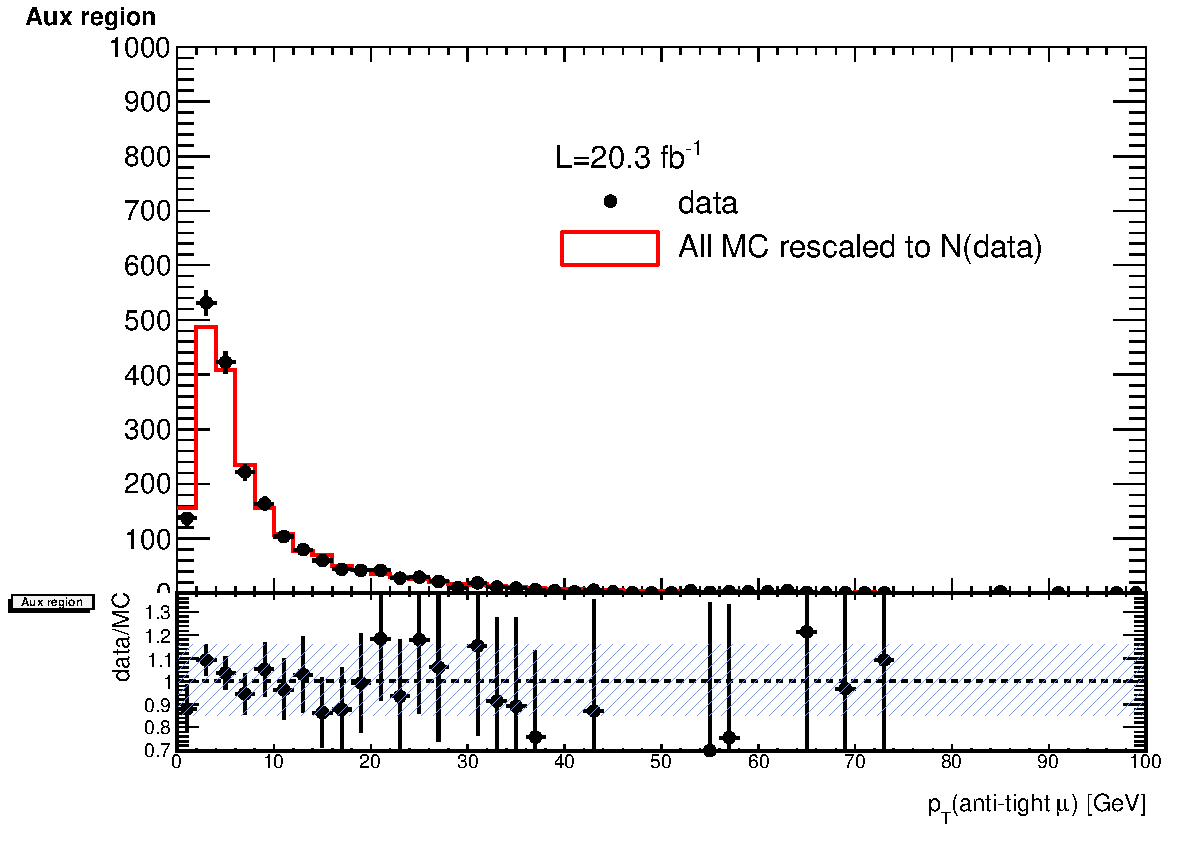
\includegraphics[width=\textwidth]{figs/fake/h_muPt_CR_early_AF2_extrap_MET50_noIso_RESCALED}
  \end{minipage}\hfill
  \begin{minipage}[h]{0.5\textwidth}
    \centering 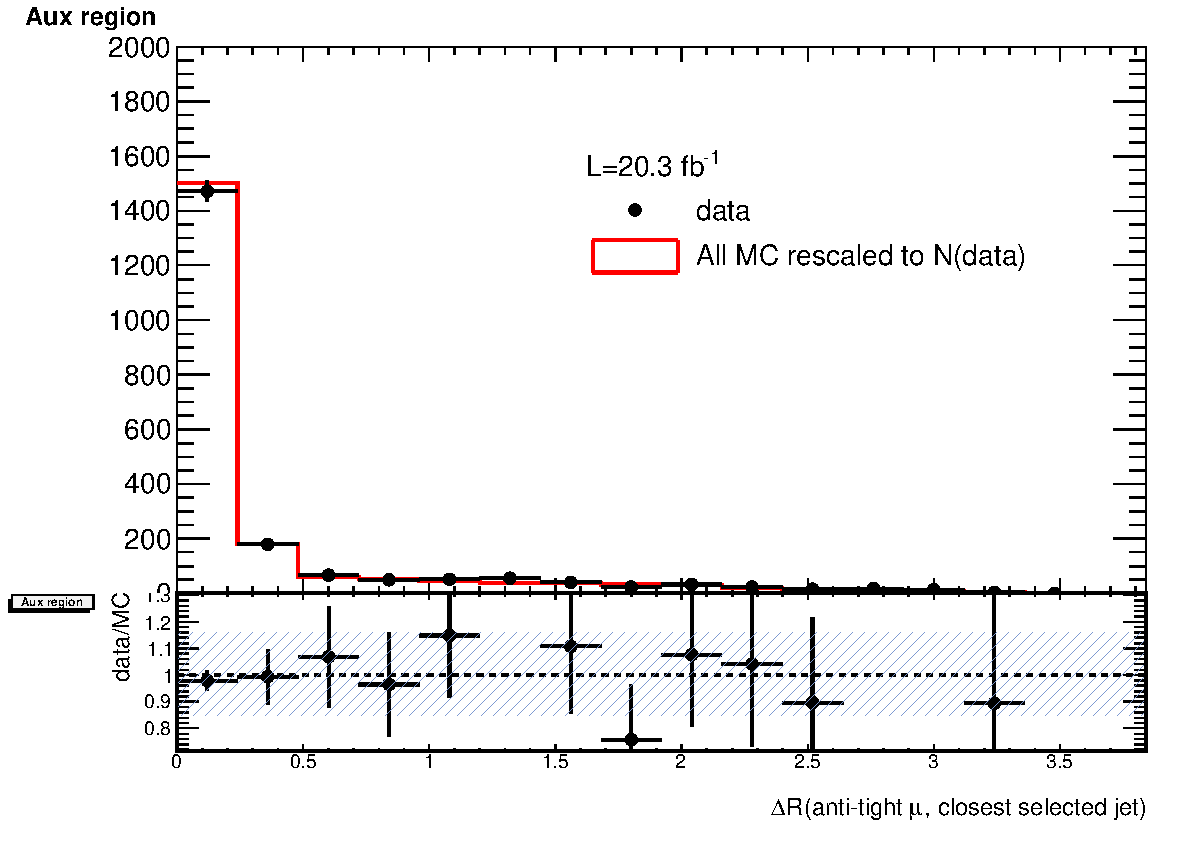
\includegraphics[width=\textwidth]{figs/fake/h_minDRjet_CR_early_AF2_extrap_MET50_noIso_RESCALED}
  \end{minipage}\hfill
  \begin{minipage}[h]{0.5\textwidth}
    \centering 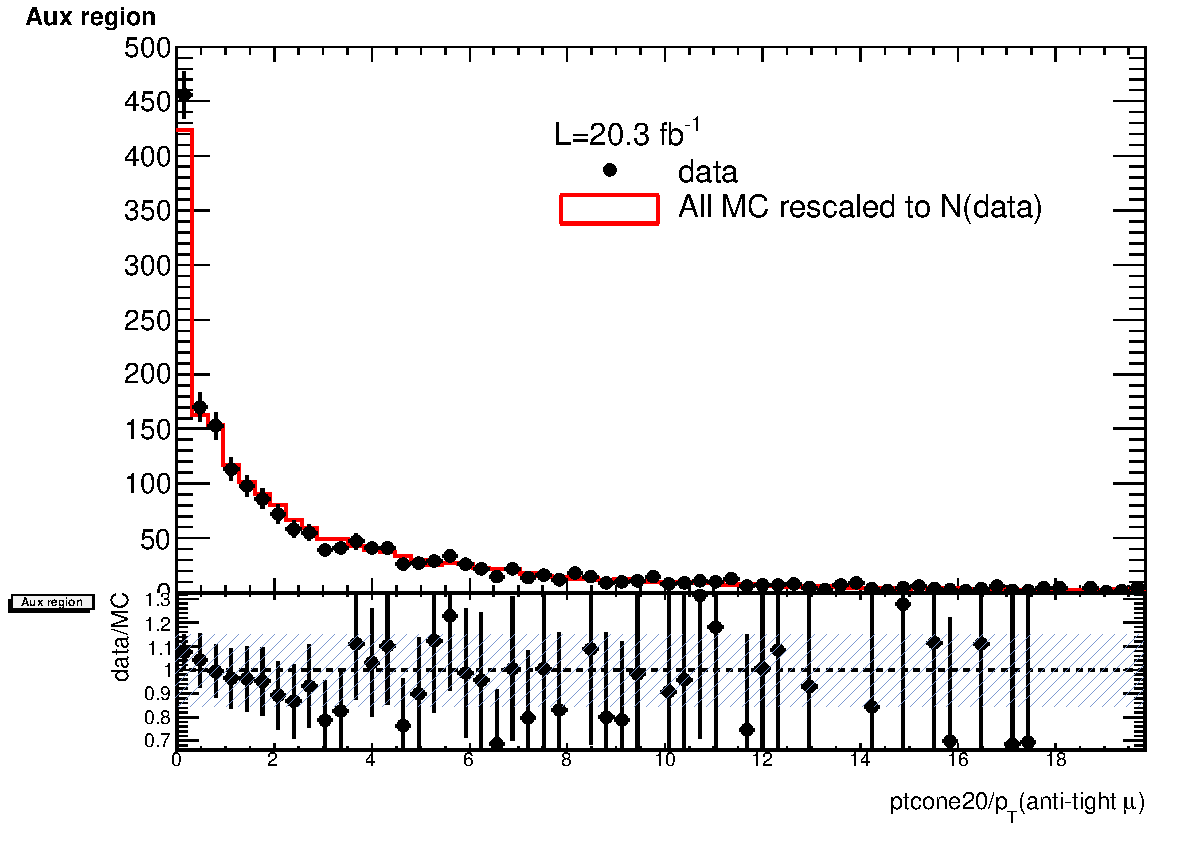
\includegraphics[width=\textwidth]{figs/fake/h_relptcone20_CR_early_AF2_extrap_MET50_noIso_RESCALED}
  \end{minipage}\hfill
  \begin{minipage}[h]{0.5\textwidth}
    \centering 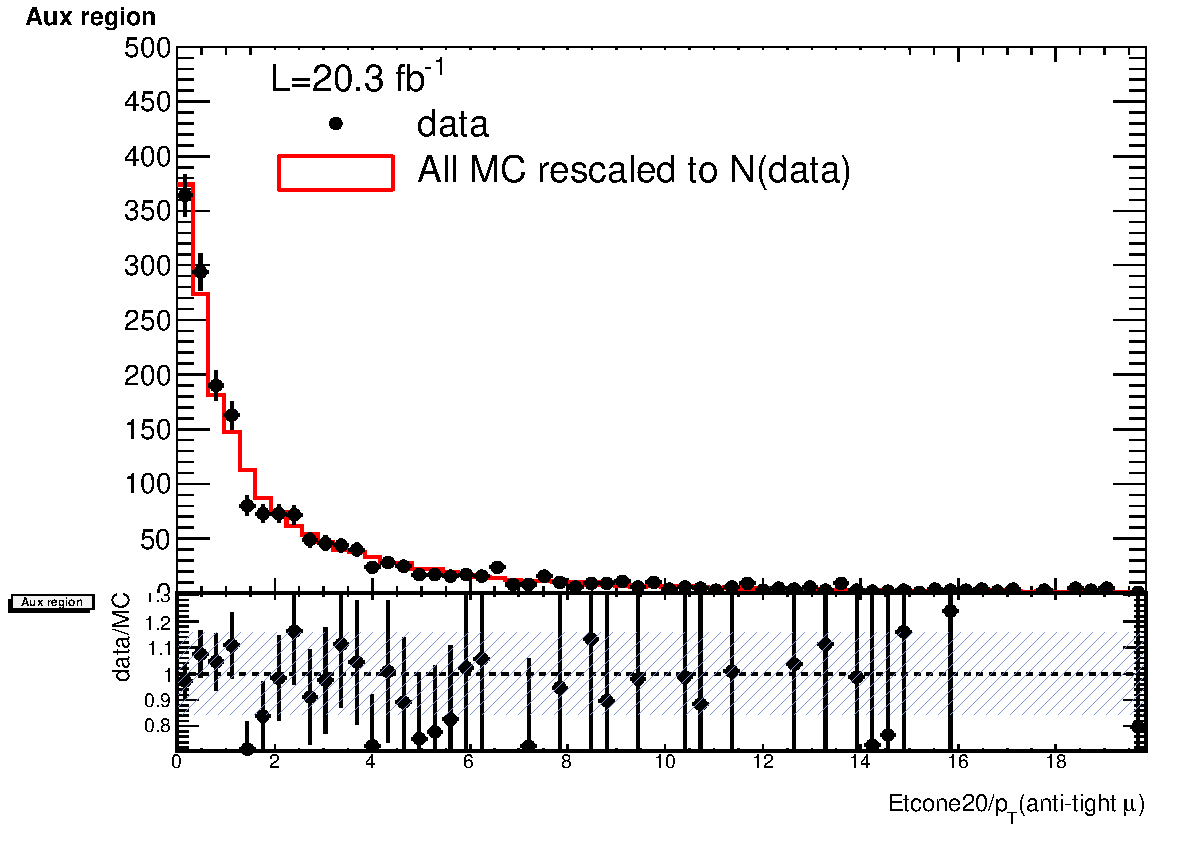
\includegraphics[width=\textwidth]{figs/fake/h_reletcone20_CR_early_AF2_extrap_MET50_noIso_RESCALED}
  \end{minipage}\hfill
  \caption{Distributions of the properties of the anti-tight muons in data (dots), compared with the total simulation (red line), rescaled to the integral of the data for a shape comparison. The uncertainty on the data distribution is statistical. The number of events for each of them is also presented in the legend. The variables probed are, top: $p_T$ and $\Delta R(\mu, {\rm , closest \, selected \, jet})$; bottom: ptcone20/$p_T$ and Etcone20/$p_T$. The selection is the signal region event selection with one anti-tight muon (failing at least one of the isolation, muon-jet overlap, or \pt\ selection criteria). A ratio plot is containing the $20\%$ area around 1, is displayed, demonstrating that a 20\% data-MC comparison systematic is sufficient.}
  \label{figure:background_muon_dataMC}
\end{figure} 


\begin{figure}[!htbp]
  \begin{minipage}[h]{0.5\textwidth}
    \centering 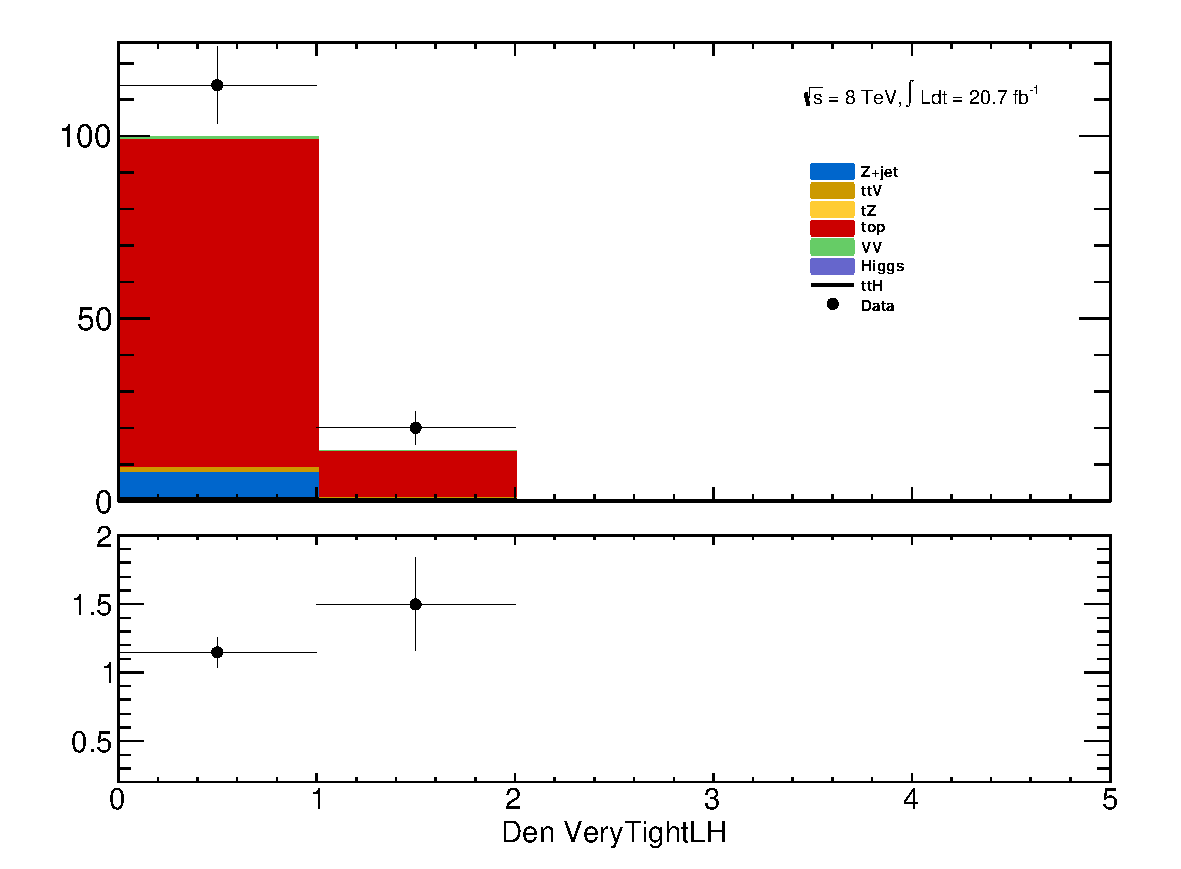
\includegraphics[width=\textwidth]{figs/fake/aux_d2_Obj0VeryTightLH}
  \end{minipage}\hfill
  \begin{minipage}[h]{0.5\textwidth}
    \centering 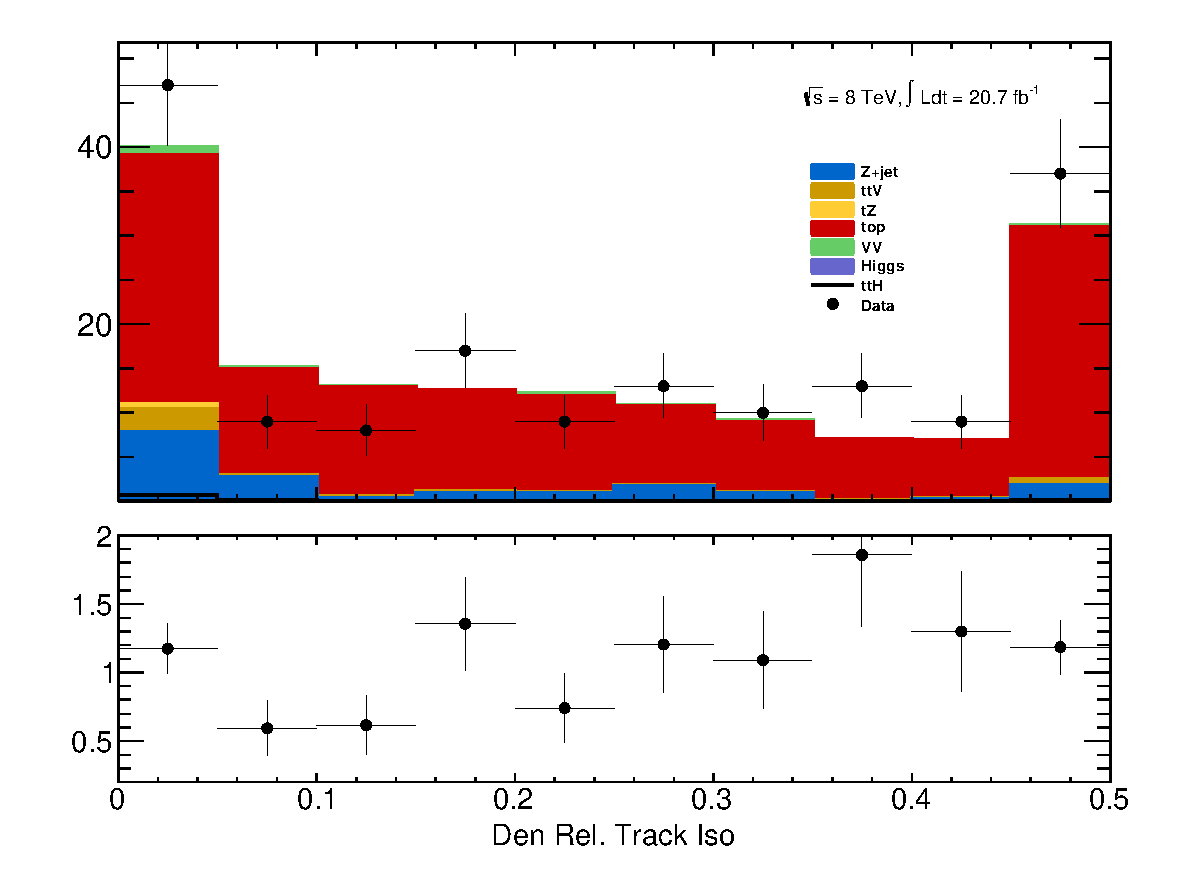
\includegraphics[width=\textwidth]{figs/fake/aux_d1_Obj0PtIso20Rel}
  \end{minipage}\hfill
  \begin{minipage}[h]{0.5\textwidth}
    \centering 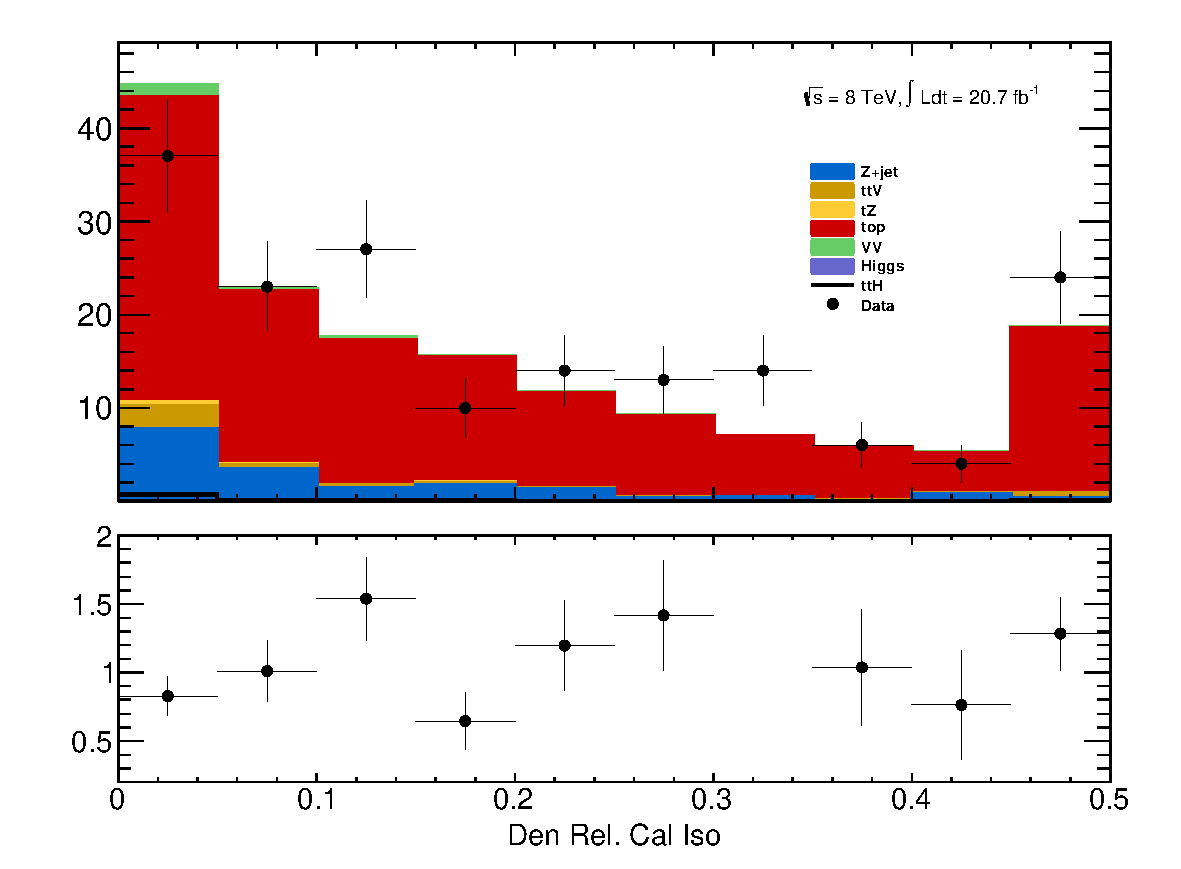
\includegraphics[width=\textwidth]{figs/fake/aux_d1_Obj0EtIso20Rel}
  \end{minipage}\hfill
  \caption{Distributions of anti-tight electron variables. The variables presented are, from top left to bottom right, $p_T$, $\eta$, \textsc{verytight} Likelihood value, ptcone20/$p_T$, Etcone20/$p_T$. The plotted regions have the same cuts as the signal region, except the anti-tight electron must fail isolation for the plot of the \textsc{verytight} identification word or fail the \textsc{verytight} identification word for the plots of the isolation. Data (dots) are compared with a stacked histogram of the various simulated samples: top in red, $V$+jets (blue), $VV$ (purple) and \ttV\ (yellow). The uncertainty on the data distribution is statistical. }   
  \label{figure:background_electron_dataMC}
\end{figure} 
%

The electron and muon anti-tight control regions, which are scaled by the transfer factors are shown in Figure \ref{figure:background_3lcr}. The prompt MC subtracted data in these regions are scaled by the transfer factors to obtain the overall contribution of fake electron and muon events in the signal region. The systematic uncertainties are split between the statistical error on the transfer factor and normalization of the anti-tight control regions and the data-MC comparisons outlined above. For muon fakes the total systematic uncertainty is 25\% and for electrons it is 34\%. The numbers and uncertainties involved in the calculation are shown in Table \ref{table:background_3l_summary}.  


\begin{figure}[!htbp]
  \begin{minipage}[h]{0.5\textwidth}
    \centering 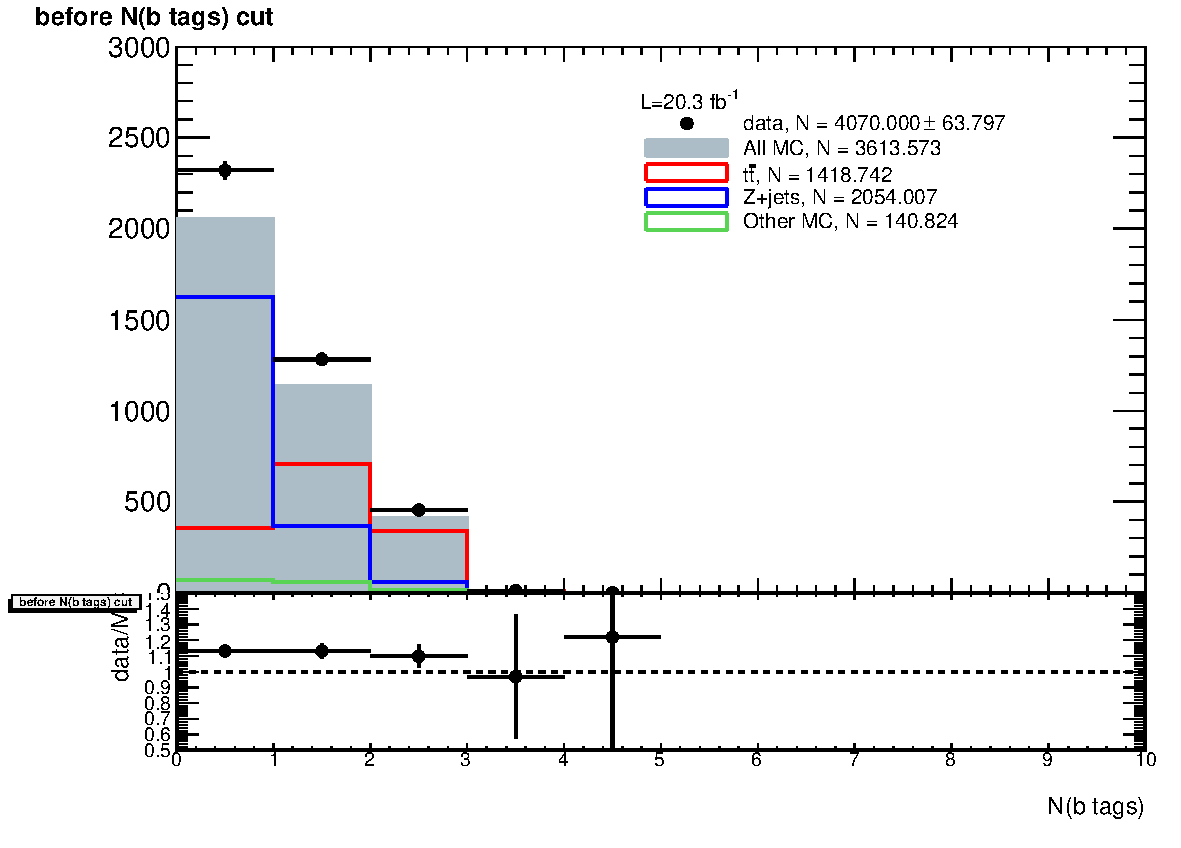
\includegraphics[width=\textwidth]{figs/fake/h_nBtags_CR_AF2_fakesCR1_noOR}
  \end{minipage}\hfill
  \begin{minipage}[h]{0.5\textwidth}
    \centering 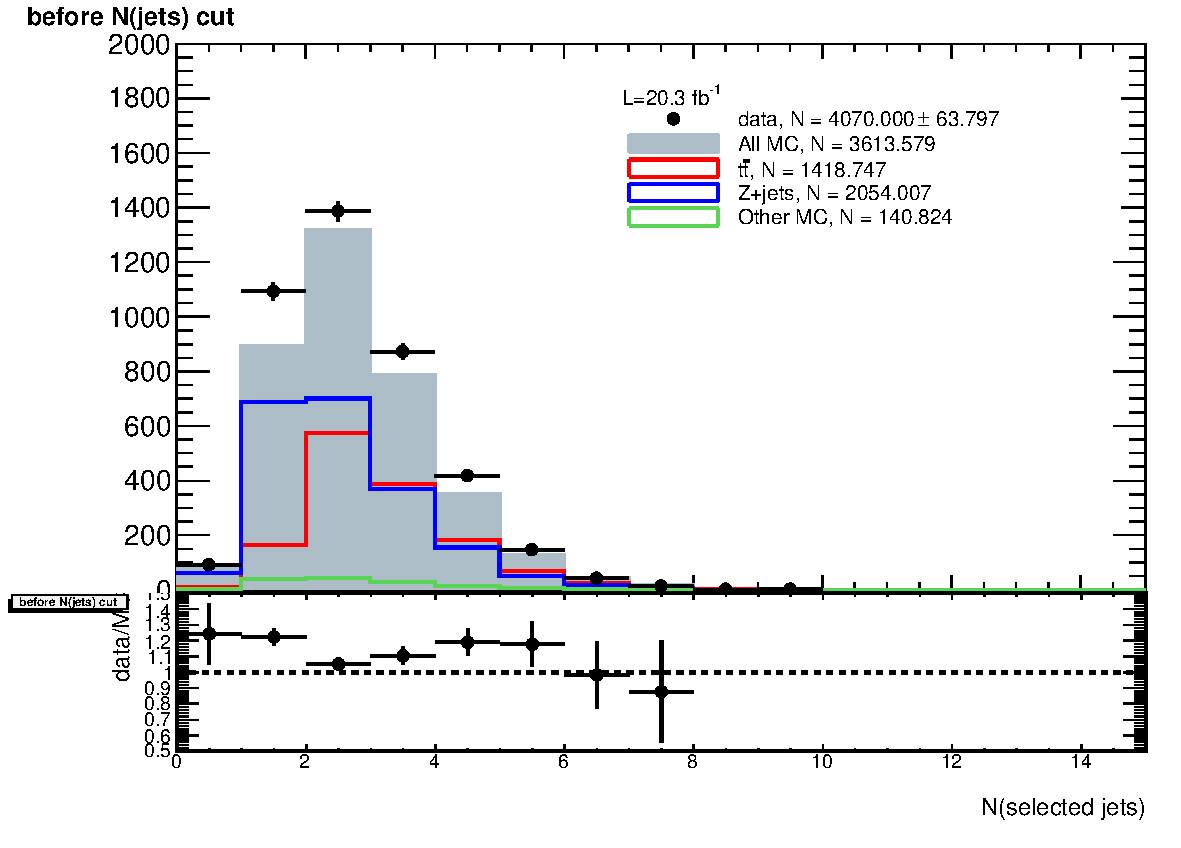
\includegraphics[width=\textwidth]{figs/fake/h_nJets_CR_AF2_fakesCR1_noOR}
  \end{minipage}\hfill
  \begin{minipage}[h]{0.5\textwidth}
    \centering 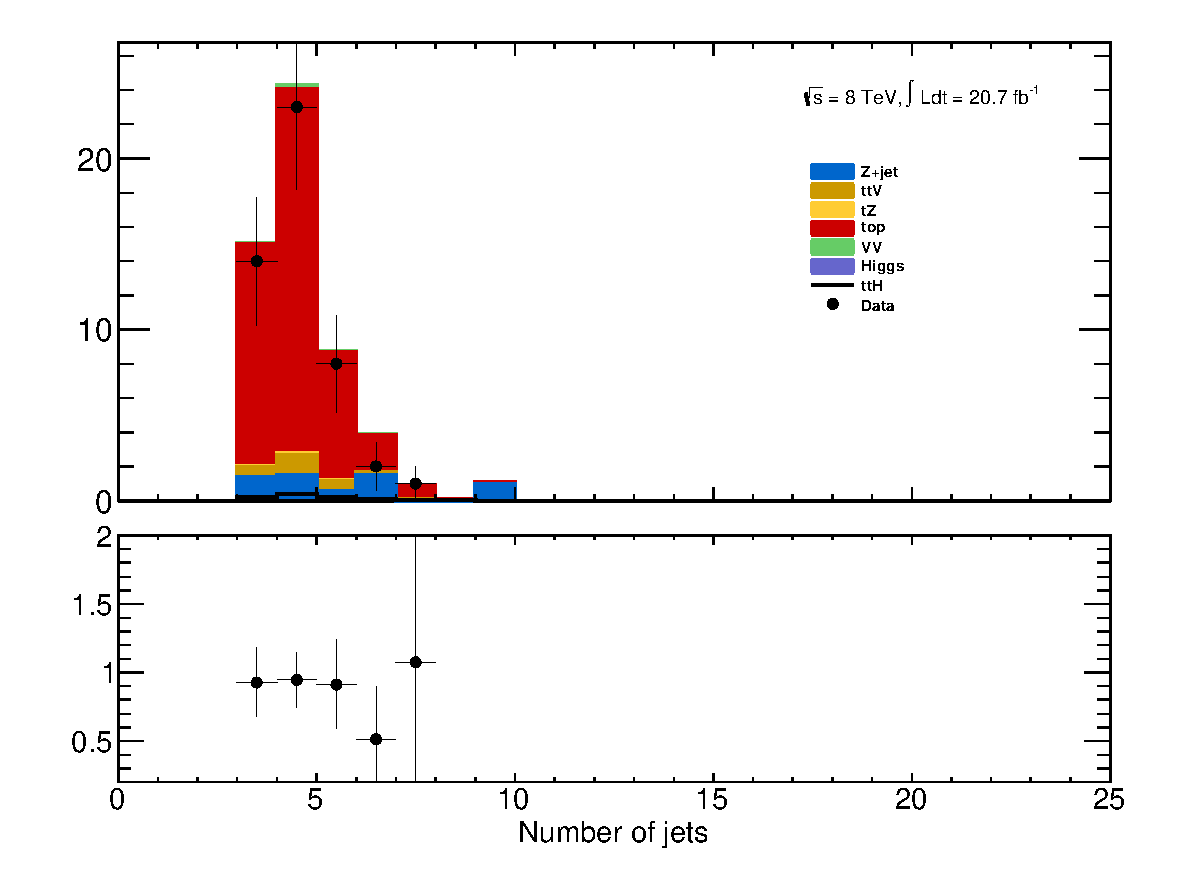
\includegraphics[width=\textwidth]{figs/fake/cr_d1_NJet}
  \end{minipage}\hfill
  \begin{minipage}[h]{0.5\textwidth}
    \centering 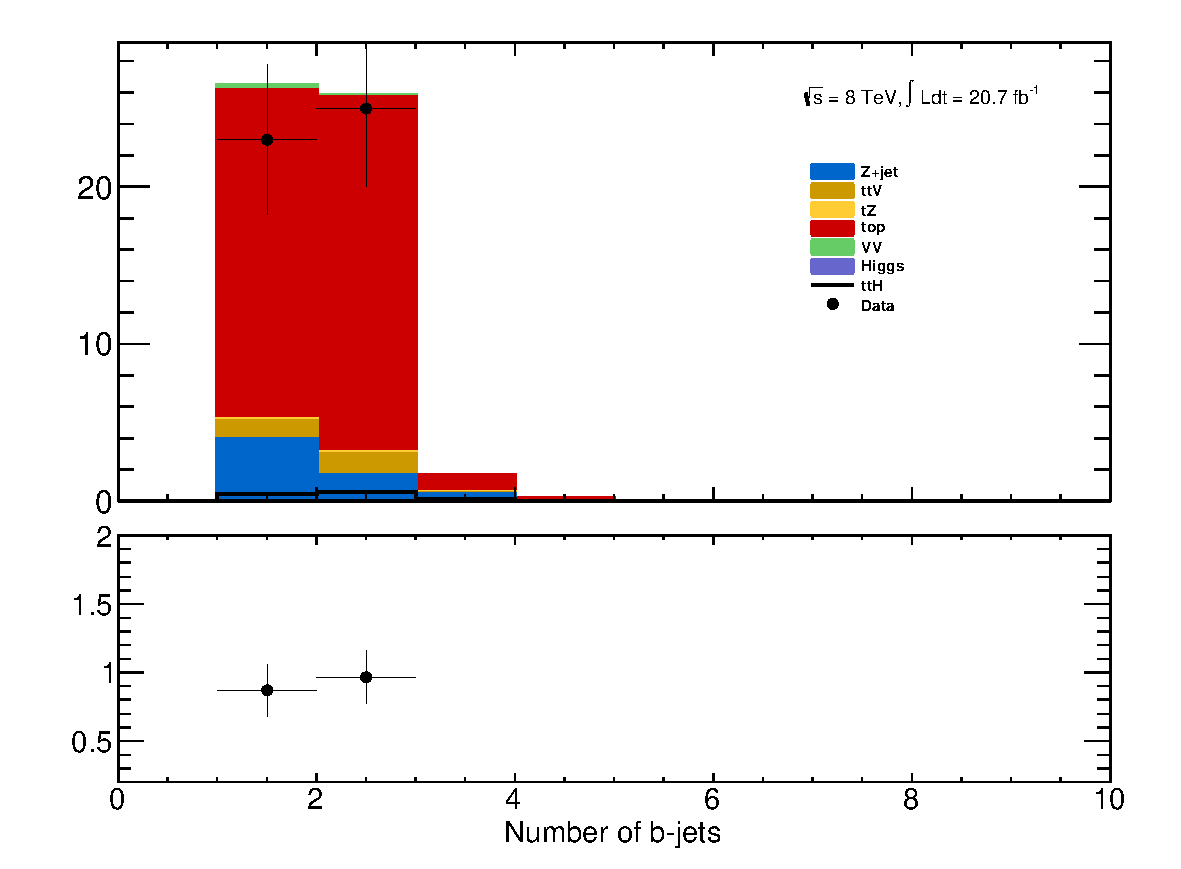
\includegraphics[width=\textwidth]{figs/fake/cr_d1_NJetBTag}
  \end{minipage}\hfill

  
  \caption{Muon-xxp (above) and electron-xxd (below) anti-tight control regions: jet variables. Note: the \ttbar\ and single top MC in the plots is used only as comparison, but is not included
  in the fake measurement}
  \label{figure:background_3lcr}
  \end{figure} 

\begin{table}[!htbp]
\begin{center} 
\begin{tabular}{|c|c|c|} 
  \hline
  Stage   & Muon & Electron \\
  \hline
  Anti-Tight CR Normalization  &  364.62 $\pm$ 20.02 (5$\%$) & 38.2 $\pm$ 6.9 (17\%) \\ 
  \hline  
  Transfer factor  & $0.0047 \pm 0.0011$ (23$\%$) & 0.0240 $\pm$ 0.0064 (36\%) \\
  SR Contribution & 1.71 $\pm$ 0.42 (25\%)           & 0.91 $\pm$ 0.35(39\%) \\ 
  \hline  
\end{tabular}
\caption{Summary of regions and inputs to the extraction of the number of \ttbar\ events with a fake muon in the SR}
\label{table:background_3l_summary}
\end{center}
\end{table}


The low jet region (1, 2, 3) is used as a validation for the method. The \ttbar\ and single top fakes in this region are estimated using the procedure above. Similar systematics are assessed. This region with the fake estimate is plotted in Figure \ref{figure:background_3lvaldiation}. The agreement of data and summed prediction for the fakes and prompt backgrounds is well within the systematic and statistical uncertainties. The figure also shows the same region with relaxed \pt\ cuts on all leptons to 10 GeV, which enriches the fake contributions greatly.   The data and summed fake and prompt predictions are also well within the statistical and systematic uncertainties.


\begin{figure}[!htbp]
  \begin{minipage}[h]{0.5\textwidth}
    \centering 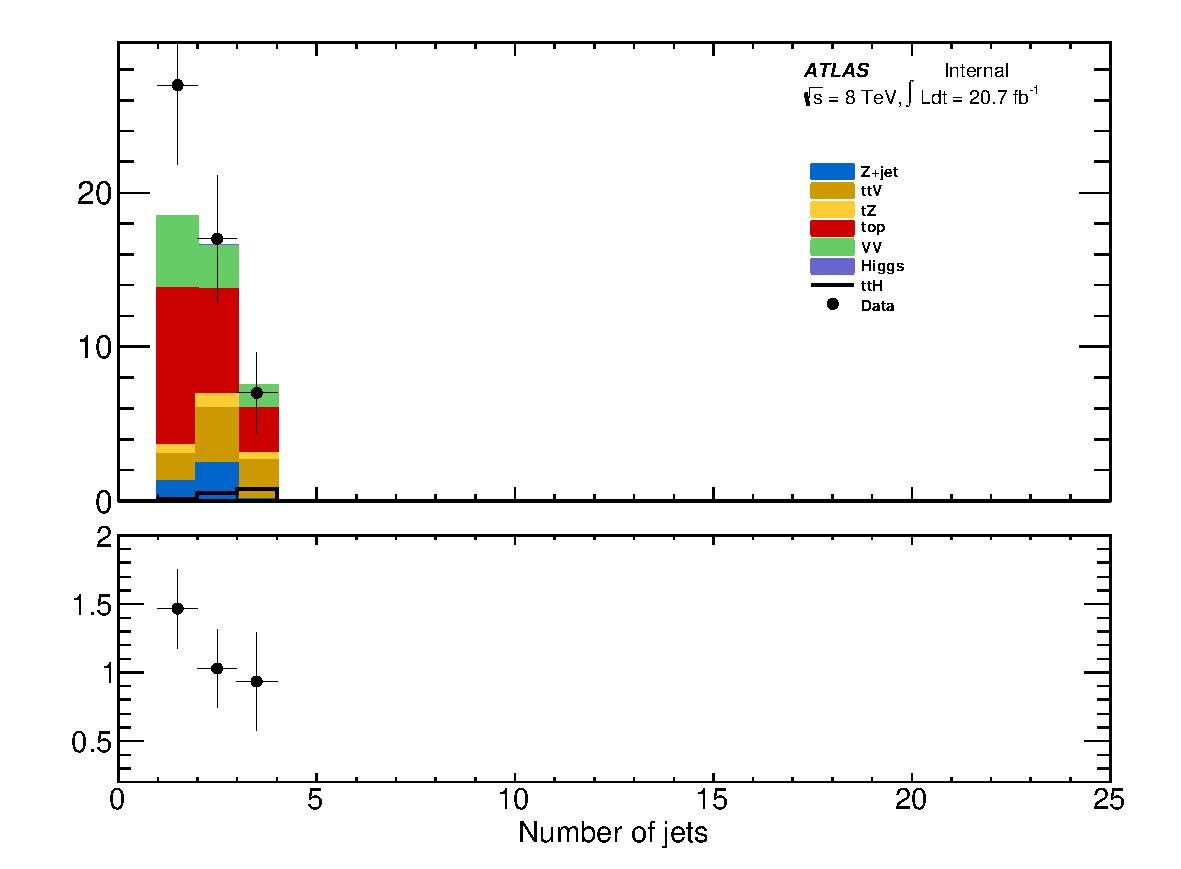
\includegraphics[width=\textwidth]{figs/fake/plotCand_3lep_C_NJet}
  \end{minipage}\hfill
  \begin{minipage}[h]{0.5\textwidth}
    \centering 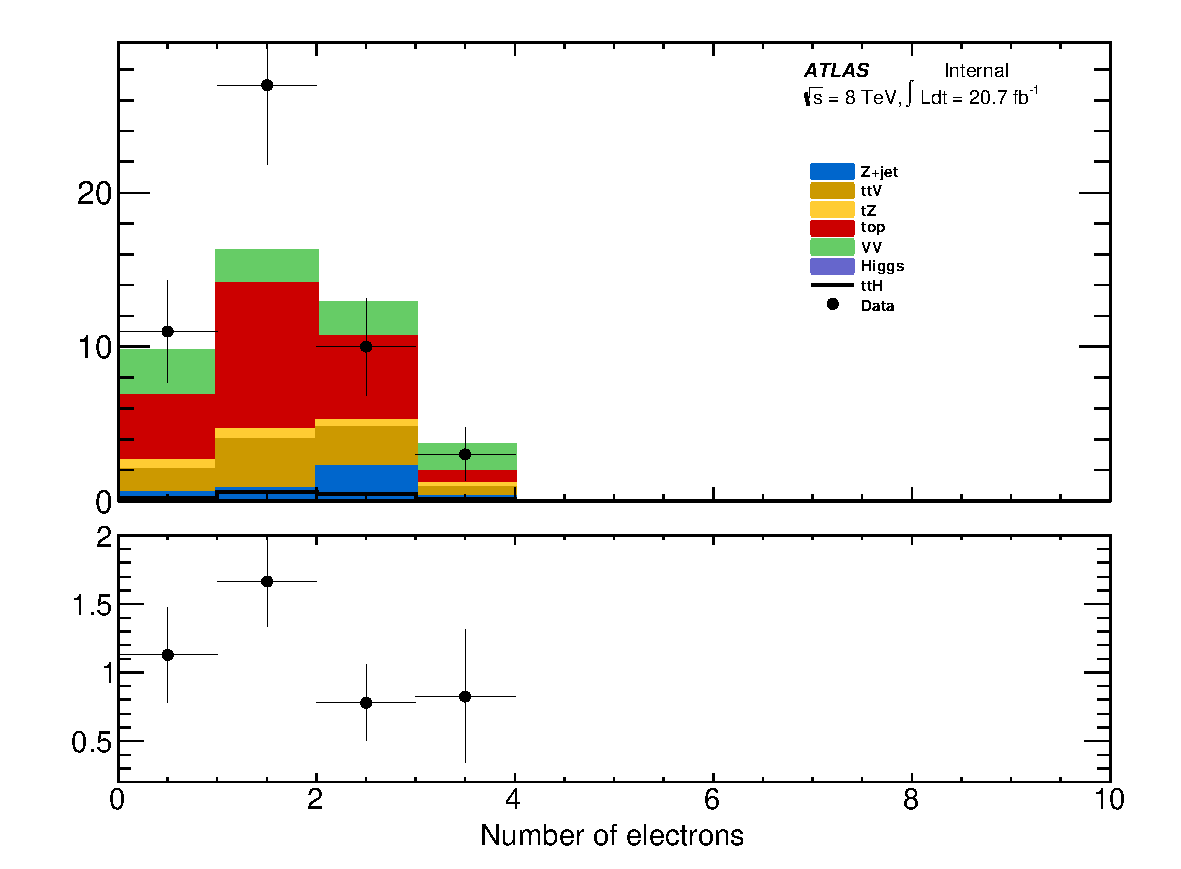
\includegraphics[width=\textwidth]{figs/fake/plotCand_3lep_C_NElec}
  \end{minipage}\hfill
  \begin{minipage}[h]{0.5\textwidth}
    \centering 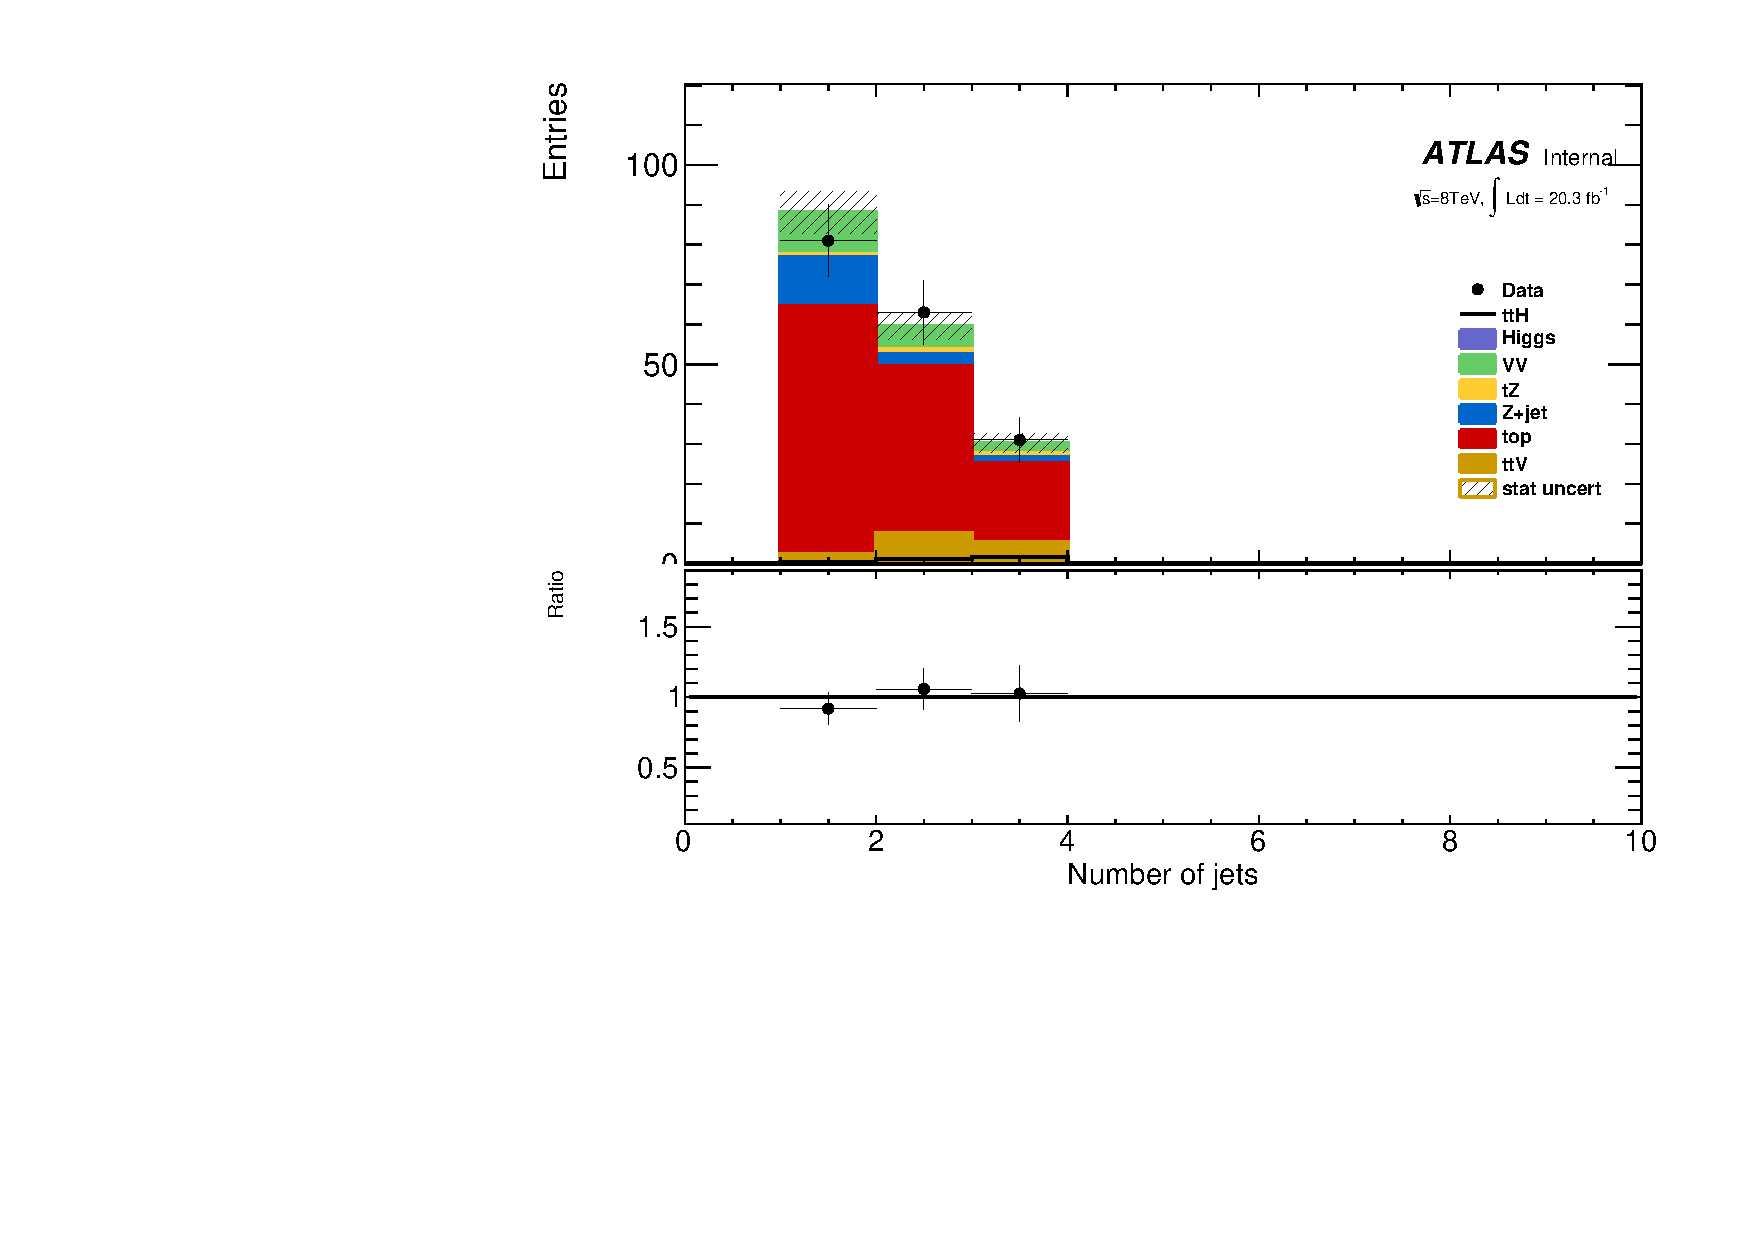
\includegraphics[width=\textwidth]{figs/fake/plotCand_3lep_LowNJet_NJet}
  \end{minipage}\hfill
  \begin{minipage}[h]{0.5\textwidth}
    \centering 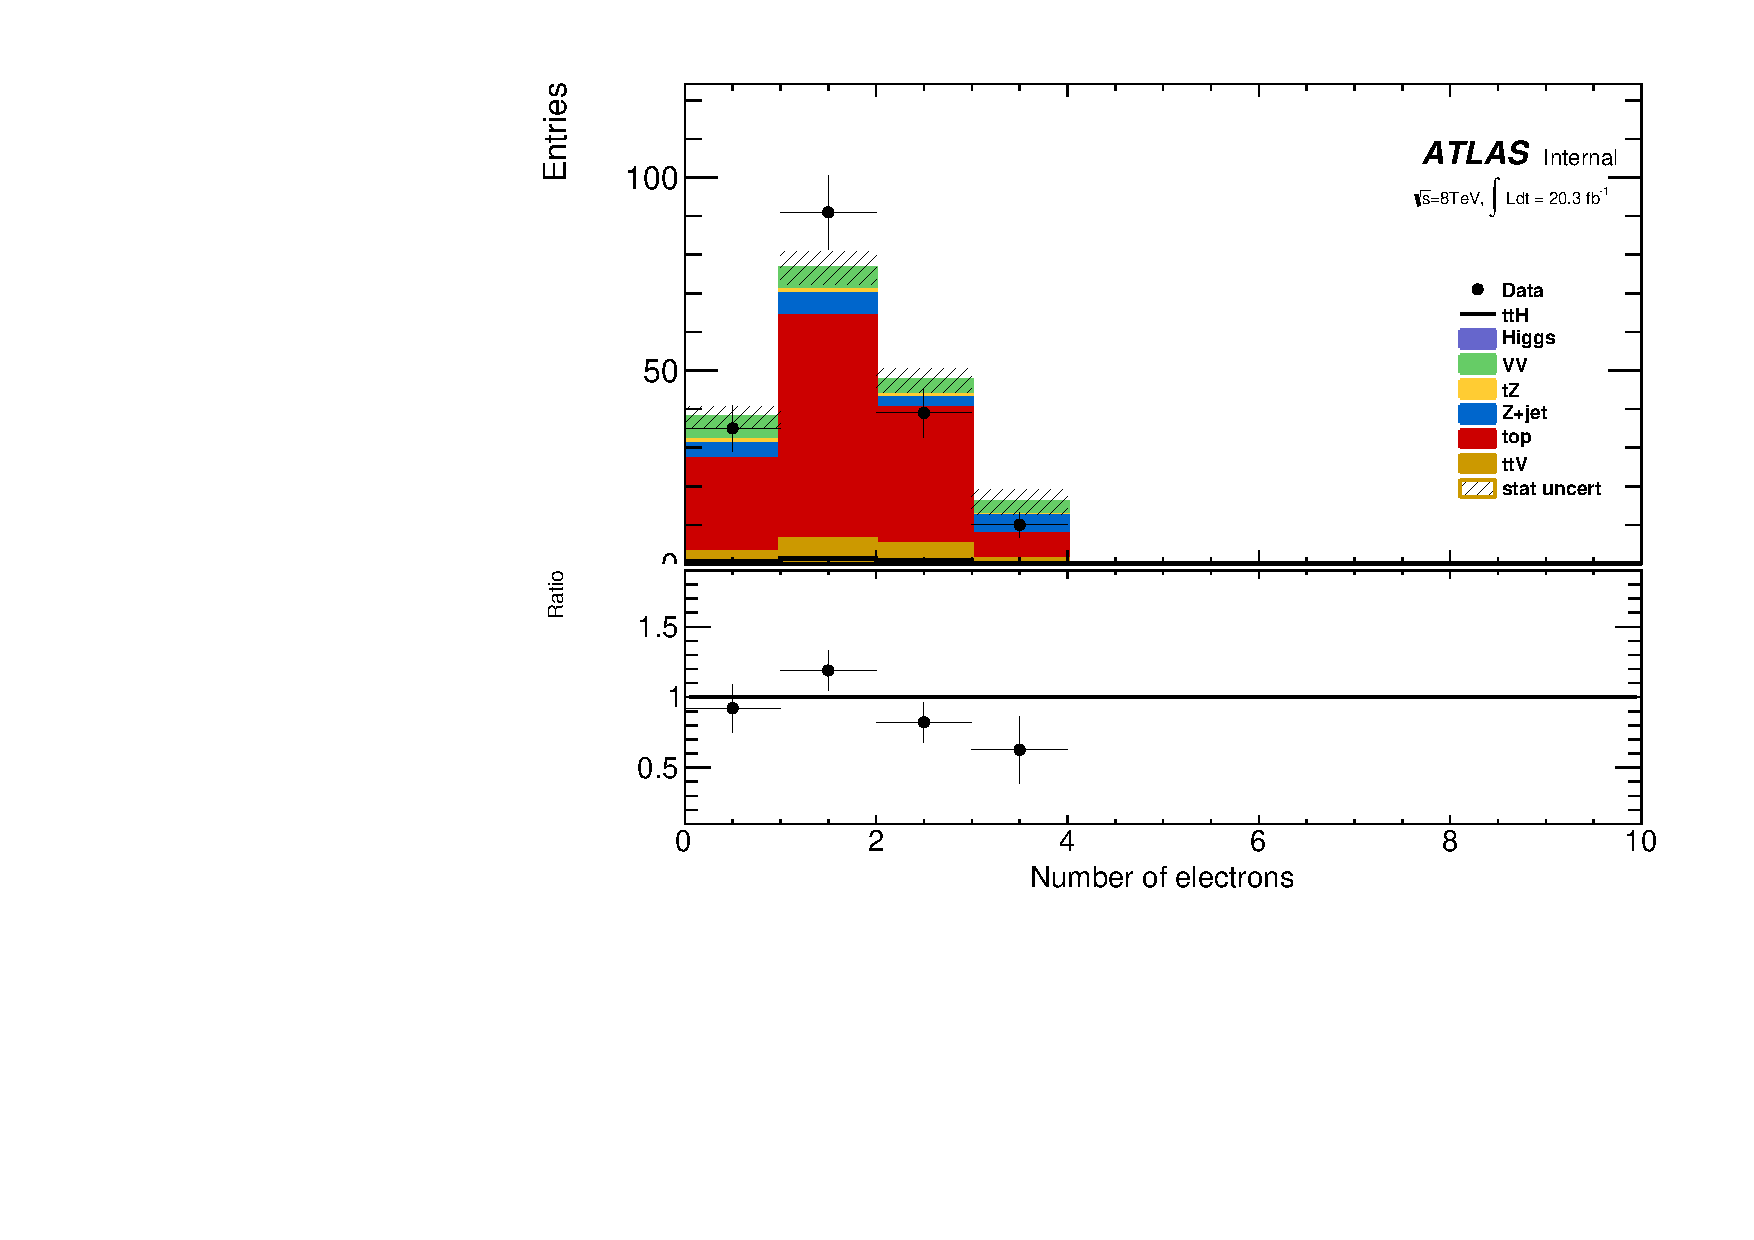
\includegraphics[width=\textwidth]{figs/fake/plotCand_3lep_LowNJet_NElec}
  \end{minipage}\hfill
  \caption{ 3$\ell$ fake validation regions for nominal \pt\ selection (above) and relaxed \pt\ selection, $>$ 10 GeV, (below). Plotted are the number of jets and the number of electrons in each event. The data and MC ratio below each plot agree with 1 within the statistics of the region and the overall systematic assigned for the fake component (red)}  
  \label{figure:background_3lvaldiation}
\end{figure} 



\subsection{4$\ell$ Fakes}

We will not discuss the 4$\ell$ fakes in depth, as it is a very small background - at the \% level and will have almost no impact on the final result. The fake method used in the the 4$\ell$ case is similar to the 2$\ell$ and 3$\ell$ cases discussed above. All fakes arise from \ttbar\ and single-top events, where \textit{two} jets are misidentified as leptons. To measure the contribution of this background, control regions with 2 fully identified and 2 anti-identified leptons are created. These control regions do not have a number of jets requirement in order to increase statistics.  From these control regions, two extrapolations are made. First, a transfer factor is applied to extrapolate from the anti-tight to tight regions for electrons and muons. The regions are defined with identical object identification selection and reversal as the 3$\ell$ case, and the same transfer factors can be used. They must be used twice however, because there are two anti-identified leptons in each event. Second, the jet inclusive regions are extrapolated into the 2-jet signal region, using a second extrapolation factor derived from \ttbar\ events. Since, the majority of fake leptons arise from b-quark initiated jets, the jet spectrum \ttbar\ events with the additional requirement of 2-b-tagged jets from data are used as a model for the jet extrapolation. The overall systematic uncertainty on this measurement arises from the statistics in the control regions and MC based assessments of non-closure and are 35\%-50\% depending on the sub-channel. 


